\NeedsTeXFormat{LaTeX2e}[1995/12/01]
\ProvidesFile{ubcsample.tex}[2012/04/07 v1.70 ^^J
 University of British Columbia Thesis]
\PassOptionsToPackage{demo}{graphicx}
\documentclass[msc,oneside]{ubcthesis}

% \afterpage{\clearpage} right after a figure.  
\usepackage{afterpage}
\usepackage{float}
\usepackage{longtable} % to define tables that span multiple pages.
\usepackage{pdflscape} % allows for landscape format pages
\usepackage[numbers,sort&compress]{natbib}
\usepackage{psfrag}
\usepackage{graphicx} % for pdf, bitmapped graphics files
\usepackage{amsmath} % assumes amsmath package installed
\usepackage{amssymb}  % assumes amsmath package installed
\usepackage{caption}
\usepackage{subcaption}
\usepackage{multirow}
\usepackage{comment}
%\excludecomment{figure}
%\let\endfigure\relax
%\usepackage{subfigure} % include multiple figures and captions within a single figure environment.
%\usepackage{here}
%\usepackage[subfigure, titles]{tocloft} % This allows you to use math in graph labels
%\usepackage{alltt} % This is useful for including source code from an additional file.
%\usepackage{listings} % has facilities for pretty-printing many languages.

\usepackage[unicode=true,
  linktocpage,
  linkbordercolor={0.5 0.5 1},
  citebordercolor={0.5 1 0.5},
  linkcolor=blue]{hyperref}
%\newcommand\url[1]{\texttt{#1}} % put the URL's in a typewriter font but not link them (comment hyperref first)

\usepackage{setspace}
%\singlespacing
\onehalfspacing
%\doublespacing

\newfloat{Program}{h}{lop}

\institution{The University Of British Columbia}
\faculty{The Faculty of Graduate and Postdoctoral Studies}
\program{Computer Science}
\institutionaddress{Vancouver}
\previousdegree{B.CS. Hons. Co-op, The University of Manitoba, 2011}
%\title{Mapping Environment Properties to Sensory Inputs for Robotic Manipulation}
\title{Real-time Predictions from Unlabeled High-Dimensional Sensory Data during Non-prehensile Manipulation}
\author{Daniel Michael Troniak}
\copyrightyear{2014}
\submitdate{\monthname\ \number\year} % The "\ " is required 

\renewcommand\thechapter      {\arabic{chapter}}
\renewcommand\thesection      {\thechapter.\arabic{section}}
\renewcommand\thesubsection   {\thesection.\arabic{subsection}}
\renewcommand\thesubsubsection{\thesubsection.\arabic{subsubsection}}
\renewcommand\theparagraph    {\thesubsubsection.\arabic{paragraph}}
\renewcommand\thesubparagraph {\theparagraph.\arabic{subparagraph}}

\setcounter{tocdepth}{2}
\setcounter{secnumdepth}{2}

\begin{document}

\frontmatter
\maketitle                      %% Mandatory

\begin{abstract}                %% Mandatory -  maximum 350 words
Robots can be readily equipped with sensors that span a growing range of modalities and
price-points.  
However, as sensors increase in number and variety, making the best use of the rich multi-modal sensory streams becomes increasingly challenging. 
In this thesis, we demonstrate the ability to make efficient and accurate task-relevant predictions from unlabeled streams of sensory data for a non-prehensile manipulation task. Specifically, we address the problem of making real-time predictions of the mass, friction coefficient, and compliance of a block during a topple-slide task, using an unlabeled mix of 1650 features composed of pose, velocity, force, torque, and tactile sensor data samples taken during the motion. 
Our framework employs a partial least squares (PLS) estimator as computed based on training data. 
Importantly, we show that the PLS predictions can be made significantly more accurate and robust to noise with the use of a feature selection heuristic, the {\em task variance ratio}, while using as few as 5\% of the original sensory features. 
This aggressive feature selection further allows for reduced bandwidth when streaming sensory data and reduced computational costs of the predictions. 
We also demonstrate the ability to make online predictions based on the sensory information received to date. We compare PLS to other regression methods, such as principal components regression. 
Our methods are tested on a WAM manipulator equipped with either a spherical probe or a BarrettHand with arrays of tactile sensors.
\end{abstract}

\chapter{Preface} % Manditory if any of the conditions are met
The thesis is based on work conducted jointly between the Sensorimotor Systems and IMAGER laboratories with professors Dinesh K. Pai and Michiel van de Panne, and students Daniel Troniak and Chuan Zhu of the University of British Columbia. This section outlines the contributions of each of the above individuals. Students worked under guidance of the professors.  

\paragraph{Software}
Troniak wrote the C++ software framework for the control, perception and user interface of the robot, and developed MATLAB scripts in support of the design and usage of the TVR algorithm. Zhu implemented a MATLAB framework for data analysis, processing and figure generation, including the final implementation of the TVR algorithm. 

\paragraph{Experiments} 
Troniak designed and built the environment for the robot, collected all data with the robot, maintained and configured the hardware, and designed and executed the robot motion. Pai supported the purchase and maintenance of the robotic hardware. Zhu analyzed preliminary data collected during various manipulations to help Troniak determine successful motion trajectories. Data analysis, discussion, and final figure generation was accomplished collaboratively.

\paragraph{Algorithms}
van de Panne suggested the TVR feature selection metric and proposed the usage of the PLS algorithm. Troniak validated the effectiveness of the TVR algorithm on data collected during manipulations. Zhu performed similar validation on the usage of the PLS algorithm, as well as designed the scheme for realtime predictions using PLS.

\paragraph{Writing}
Chapters \ref{chap3}, and \ref{chap5} of the thesis are adapted from a paper submitted to the 2015 IEEE International Conference on Robotics and Automation (D Troniak, C Zhu, D Pai, M van de Panne, Real-time Predictions from High-dimensional Unlabeled Sensory Data during Non-prehensile Manipulation, ICRA 2015, submission \#1575, 01 October 2014). Troniak performed and wrote the background literature review and drafted the remainder of the manuscript, which was then improved and prepared for submission by van de Panne.

\paragraph{Figures}
Figure \ref{fig:eg_sensor_trace} was generated by Troniak. Part of Figure \ref{fig:topple} was designed by van de Panne and is present in the paper submitted to ICRA 2015. 
%TODO
Figures from Chapter~\ref{chap5} were developed collaboratively and are also present in the paper. Figures borrowed from the literature include appropriate references within the caption.


\tableofcontents                %% Mandatory
\listoftables                   %% Mandatory if thesis has tables
\listoffigures                  %% Mandatory if thesis has figures
%% Any other lists should come here, i.e. definitions, glossary, list of symbols etc.

\chapter{Acknowledgements}      %% Optional
%This thesis would not have been possible if not for my supervisors Professor Dinesh Pai and Professor Michiel van de Panne, whose guidance, patience and trust allowed me to guide this project to its full potential. 
%They are both phenomenal mentors, and together brought complementary perspectives to this work, enhancing both its depth and breadth. 
%Individual thanks go to Professor Pai for securing the robotic system and for providing high-level direction and feedback, and to Professor van de Panne for providing concrete instruction and for never failing to find ample time in his busy schedule for stimulating discussion.

%Thanks also to Chuan Zhu, my lab-mate, with whom I shared much elation (and dissapointment!), for providing encouragement and comedy in the late-hours before deadlines. I also wish to thank Prof. Pai and Prof. Ian Mitchell, who, through their project courses (CPSC548 and CPSC515) at UBC, allowed me to pursue my interests in the early stages of my graduate career which eventually led me my current focus of study.  

%Special thanks to Professor van de Panne and all members of the MOCCA reading group for listening to my (sometimes mundane) talks on topics related to my thesis. Similar thanks go to Professor Pai and the SMRT reading group for helping me guide topics in Neuroscience into this thesis.

%Last but certainly not least, I would like to thank my family, both in Canada and in Taiwan, for their tireless effort to keep me secure, well-rested (and well-fed!) during the process of writing this thesis.



\chapter[Dedication]{} %% Optional
\emph{To Jill and Jade.}

\mainmatter % Now regular page numbering begins.

% Chapters are the next main unit.
\chapter{Introduction}
\label{chp:intro}

We begin this chapter by introducing robotic manipulation using force and tactile sensors, and present the challenges in programming robots to perform manipulation tasks in the physical world.
Following this, we state the specific problem we wish to address in this thesis as well as the motivations behind seeking its solution.
The chapter concludes with main contributions and thesis structure.

%%%%%%%%%%%%%%

\section{Learning to interact with the real world}

Our world is infinitely complex.
%; a setting in which developing complete models, i.e. all rules which govern all things, is infeasible.
By the second law of thermodynamics, any real-world system constantly changes as energy transfers between its composing particles of matter \cite{zubarev1974nonequilibrium}. 
Thus, if one's goal is to interact with such a dynamic ever-changing world, one needs to continually infer relevant truths which exist in that world through some form of external sensing.

This type of approach to system identification and control is known as \emph{model-free} \cite{Spall1998} in the sense that one functions without needing explicit knowledge of physics.

Living organisms are known to take this approach \cite{dayan2008decision}. %when interacting with the real world.
A child does not learn to walk given absolute knowledge of the dynamics which govern his interaction with the environment. Rather, he must build an action-consequence model of the walking task through much trial and error.

By learning a model which maps sensory information to relevant properties of an environment, the entity also gains an ability to predict anomalies.
% within its environment.
Novel events are important as they present opportunities to gain deeper insight into the true underlying principles which define the environment not presently described by the current model.

Humans, who are among the most successful of living organisms, have the ability to both model their environment and efficiently perform inference on that model using their available senses.
For a trained athlete to succeed in the game of basketball, she must learn to ignore irrelevant sensory data, such as the cheering of the crowd, and focus on more important information, such as the image of the basket on her retina.
How can she identify relevant information with respect to her current task?
We are interested in exploring how humans might accomplish this by enabling robots to possess such a skill.

%Consider the following example, a robot might lift a mass of 1kg on multiple occasions and each time experience an identical input pattern across its joint-torque sensors.
%We would like the robot to have the capacity to recognize and associate this pattern with picking up arbitrary objects of mass 1kg.
%Taking this a step further, the robot should be able to exploit the data-driven model it develops in order to guess the mass of a 5kg, 10kg or 20kg object, for example.

%%%%%%%%%%%%%%%%

\section{Problem Statement}

We wish to address the problem of supporting robotic manipulation by efficiently predicting properties of an environment using unlabeled sensory data.
The ability to predict properties of an environment, such as the mass of an object on a table, is an important prelude to closing the loop and allowing robots to adapt to unexpected change.

One barrier to achieving this goal, however, is that the size of the input space increases with the number of sensor readings available to the system.
This makes making predictions susceptible to Bellman's infamous curse of dimensionality.
We therefore take steps to reduce the number of sensors considered when predicting properties of an environment.

To test our solution, we consider a block topple-slide task (see Figure~\ref{fig:topple}) performed by a robot equipped with force, torque and tactile sensors.
In this task, the end effector of the robot pushes on the side of a foam-encapsulated block, causing it to topple, and then pushes the block back to its starting pose against a wall.
A prescribed joint-angle trajectory to achieve this manipulation task is provided by a human expert through kinesthetic teaching.
%The robot tracks the given trajectory in joint space using a standard computed-torque tracking procedure.
The given example trajectory is assumed to be robust in two ways: repeating the trajectory should cause repeated rotations of the block, and the same trajectory should remain successful when applied to blocks with variations in mass, friction, and compliance. 

%The use of a prescribed manipulation trajectory also implies an approximate correspondence between the current elapsed time within a motion and the phase of the manipulation.

\begin{figure}[]
	\centering
	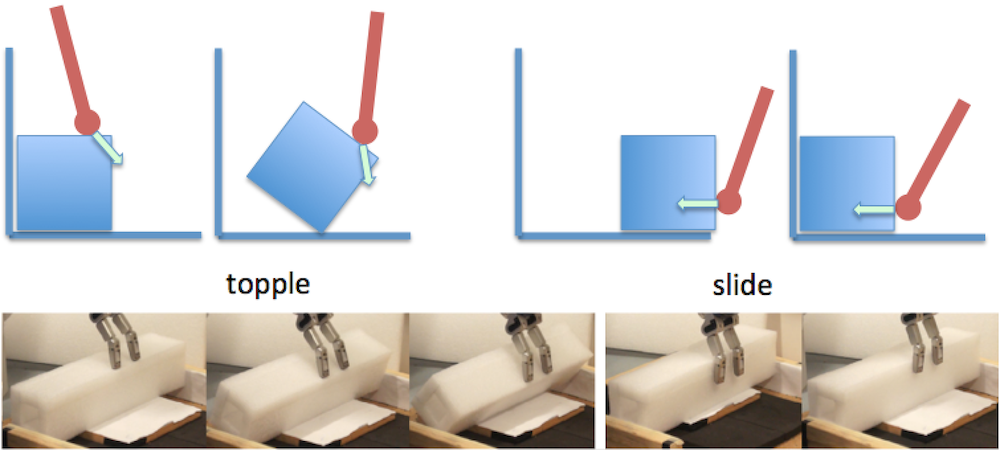
\includegraphics[width=\linewidth]{images/topple}
	\caption{The topple-slide task.}
	\label{fig:topple}
\end{figure}

%%%%%%%%%%%%%%%%%%%

\section{Motivations}
As sensing technologies become more affordable, robots will be able to concurrently make a wide range of measurements within the environments in which they operate.  
As can be seen in Figure~\ref{fig:eg_sensor_trace}, it is clear that sensors with the capacity to measure properties of an environment will obtain distinct readings as those environment properties change. 
Notice how the streams become disjoint during phases of robot-object contacts (during toppling and sliding) and recombine during phases of non-contact.
It then becomes possible, given some form of ground-truth, for the robot to learn a model which explains how changes in its sensor readings relate to changes in its environment.

%Consider a concrete example: the robot may develop a mapping between (1) sensory data traces while handling a piece of fruit and (2) the level of ripeness of the fruit.
%When the robot encounters a piece of fruit that affords a familiar sensory experience (i.e. near previous samples of the sensory input space), the robot has the capacity to classify that piece of fruit as having a particular level of ripeness.

This releases the need for experts to model the relationships between sensory readings and environmental phenomena. 
For example, distinct force measurements may relate to the compliance of an object, which in turn could provide insight into some high-level feature such as its ripeness (if the object were a piece of fruit).
We thereby achieve a highly scalable system capable of mapping arbitrary sensor readings (vision, olfactory, inertial, etc.) to arbitrary environment properties, given the availability of relevant ground-truth information on which to train the model-learning system.

%FIGURE
\begin{figure}[hbt]
	\centering
	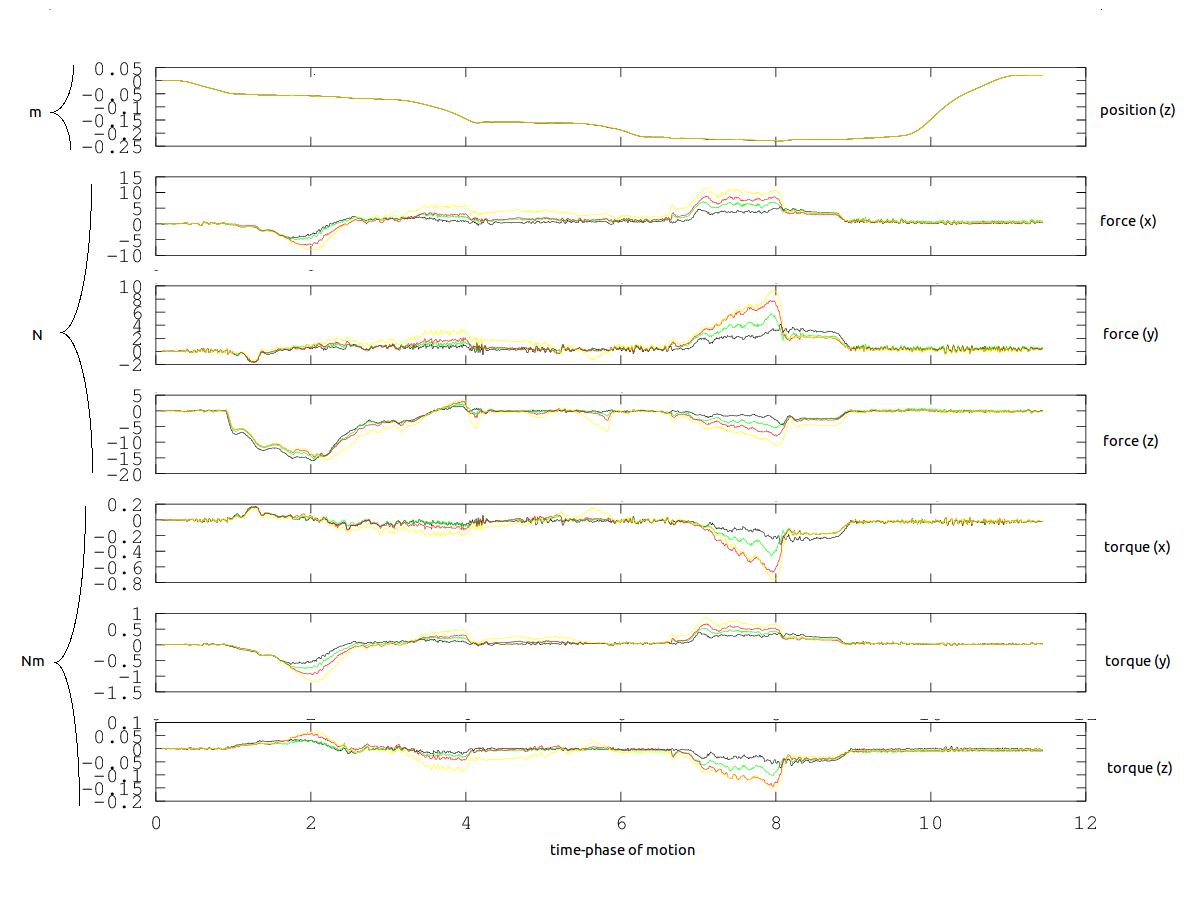
\includegraphics[width=\linewidth]{images/eg_sensor_trace}
	\caption{Example sensory streams during the topple-slide task in different environments (one colour for each environment).
}
	\label{fig:eg_sensor_trace}
\end{figure}
%ENDFIGURE

%%%%%%%%%%%%%%%%%%%



%%%%%%%%%%%%%%%%%%

\section{Contributions}
The contributions of this thesis are three-fold: 
(1) a unifying bridge between literature in robotics, physiology and neuroscience on the topic of exploiting force and tactile sensors for dexterous manipulation, 
(2) an unsupervised feature selection algorithm based on a new metric called the task variance ratio, which filters important sensor readings and motion-phases within high-dimensional sensory data streams during manipulation tasks and 
(3) a supervised learning algorithm with partial least squares (PLS) regression at its core, which builds statistical data-driven models that use important sensory data traces from a robot to predict properties defining its environment.

The feature selection algorithm allows the robot to distinguish between sensors which provide task-critical information, and sensors which provide information that is noisy or irrelevant to the task.
This ability to gauge the usefulness of sensor readings becomes important as the number of sensors in the system increases, and real-time processing of all sensors becomes impossible.
Disregarding all but the most important sensors reduces algorithmic complexity to constant time, which guarantees support for real-time operation irregardless of the number of sensors physically available to the robot.
The developed models are then used to efficiently predict environment properties when novel sensory data traces are recorded by the robot's sensors.

%%%%%%%%%%%%%%%%%%

\section{Thesis Structure}
Following this introductory chapter, we provide background literature on the topic of exploiting force and tactile sensor data for manipulation in the robotics, neuroscience and physiology literature in Chapter~\ref{chap2}.
In Chapter~\ref{chap3}, we more formally define the algorithms and data structures used in our approach.
Chapter~\ref{chap4} contains an overview of the software developed in support of experiments.
In Chapter~\ref{chap5}, we present experimental procedures and results of experiments with the physical robotic system.
Finally, conclusions are drawn in Chapter~\ref{chap6}.

\chapter{Background}
\label{chap2}

\section{Robotic Manipulation}

In the present study, we consider the general research question: how should robots be programmed to manipulate (e.g. grasp) objects? 
There exist two common approaches to this problem in the robotics literature.
One approach is for a human expert to provide the robot with an analytical model of itself and its environment. 
Using this model, the robot achieves its manipulation goals in two phases: planning and execution.
%plans an end-effector trajectory and then executes that trajectory to perform the desired manipulation.
Planning is often performed in simulation using models of object geometry and robot/environment dynamics.
Once the robot has found a feasible plan, it then executes that plan via physical robot actuation.
One disadvantage to this approach is that due to imperfect precalculated dynamical models and robot calibration, executed manipulations can easily become unstable and fail~\cite{dang2012tactile}.

%Another approach is to formulate the manipulation task as a control problem that utilizes force, torque, and tactile sensors to improve robustness.
Another approach is to remove the requirement of human-supplied models and have the models learned autonomously from data using statistical learning techniques.
The key advantage of this type of \emph{model-free} approach~\cite{Spall1998,hornung2014anomaly} is that apriori object and dynamical models are not required to succeed in the task; the model is learned automatically from data.
In this thesis, we define \emph{model-free}~\cite{Spall1998} systems as those that function without given explicit knowledge of physics or geometry from human experts.
%As well, the robot is granted the capacity to adapt to unexpected changes in the environment.
%This results in a system that is more robust to pose uncertainties without complete dependence on detailed human-calculated environmental models~\cite{dang2012tactile}.

%The latter approach is also closer to how the human motor system is known to function (see Section~\ref{high_level_processes}).  
%There is ample physiology and neuroscience literature from which inspiration and insight to devising successful manipulation schemes can be drawn based on the human sensory system, with much success already attained~\cite{felip2011emptying, leoni1998implementing, romano2011human, sikka1994tactile}.



\subsection{Model-free schemes}

%In this thesis, we define \emph{model-free}~\cite{Spall1998} systems as those that function without given explicit knowledge of physics or geometry from human experts.
%Instead, the model is learned autonomously from data using a machine learning algorithms.
%Another approach to robotic manipulation in the literature is to analyze data compiled from a series of successful manipulations and extract features from the data that are indicative of successful manipulations.
%Once these features are acquired, they can then be used to predict success in future manipulations.

One example of such a learning technique is called the Self-Organizing Map (SOM), an architecture of Artificial Neural Networks (ANN) that spatially and uniformly organizes features automatically by input signals~\cite{kohonen1990self}.
An example where SOMs have been used successfully is in~\cite{steffen2007experience}: objects are grasped based on hand posture and tactile experience of previously successful grasps.
Experience is represented as a low dimensional smooth manifold in hand posture space. 
%, which is implemented as a SOM-variant.
%Successful grasps are used to continually update the SOM experience base that is then used to guide subsequent grasps to their closest matching posture in the experience base.
%Figure~\ref{fig:grasp_som} depicts the experience base graphically.

A similar system was devised in~\cite{ratnasingam2011object}, where a SOM was used to map finger joint angles and tactile readings to object shape and size.
The system could identify previously grasped objects as well as categorize new objects as being a particular shape and size.
%The system successfully recognized 22 out of 25 different objects.

The same authors obtained similar results with another algorithm inspired by biological spiking neurons, called a spiking neural network~\cite{ratnasingam2011spiking}.
For this scheme, joint angle input is encoded into a series of spike trains which result in three feature outputs that are then used to recognize and classify grasped objects.
In addition, similar objects tended to cluster in output feature space.
% Figure~\ref{fig:sensory_clustering}).
The authors' system was able to recognize objects of different shapes as well as objects with the same shape but different size.

In~\cite{dang2011blind}, the authors present blind grasping: a novel approach to object grasping that does not require visual feedback or apriori 3D object models.
Their scheme works from a database of one thousand stable grasps from the Columbia Grasp Database~\cite{goldfeder2009columbia} using the model of a BarrettHand~\cite{townsend2000barretthand}. 
Corresponding tactile feedback during grasps of objects simulated in the Graspit!~\cite{miller2004graspit} simulator are also recorded.
%Grasps are simulated in Graspit!.
They proceed to create feature vectors comprising simulated tactile and robot kinematic data which they then use to train an SVM to classify grasps as being stable or unstable. 
%Figure~\ref{fig:tact_example} demonstrates such a feature vector as representing a stable grasp.
In this way, the system was able to learn tactile feedback indicative of a stable grasp.
%Once these successful tactile and kinematic features are learned, the robot hand can move its wrist and re-shape its hand to explore the object until similar tactile contacts to grasps in the database are achieved.

\subsection{Model-based schemes}

In \emph{model-based} schemes, a human expert provides the robot apriori models which, for example, map sensory input signals to specific control policies. 
This approach grants the advantage of providing the robot access to the understanding of the task dynamics of the researcher.
The disadvantage of this approach is that the supplied model may contain errors and is limited by the domain expertise of the researcher.
%would not generalize to aspects not specifically modeled.

In~\cite{felip2011emptying}, the authors present sensor-based atomic controllers for a robotic hand/arm system to empty a box containing an undefined number of unknown objects.
Manipulation primitives are defined that search, grasp and transport objects from the box to predefined locations.
A finite state machine (FSM) is used to transition between motion primitives based on corresponding sensory feedback.
%This FSM is presented graphically in Figure~\ref{fig:grasp_fsm}.
The authors also compare a vision-plus-tactile-based version of their system to a purely tactile-based version.
They found that while the version which incorporated vision was more efficient at completing the empty-the-box manipulation task, the tactile version was also successful.
Vision was only crucial in determining if the box was empty; in the non-vision based system, a human moderator was required to tell the robot when it had finished its task.
The authors in~\cite{felip2011emptying} also present an interesting scheme that compensates for errors in translation of the robotic hand.
The hand repositions itself if there is force experienced by only one finger, denoting a single hand/object contact.
The controller compensates by moving the hand in direction of single contact, which effectively repositions the manipulator above the object.

In~\cite{Lynch1999}, the authors take an analytical approach to the non-prehensile toppling task. 
This approach, while successful, assumes knowledge of the dynamics of the entire system and would therefore not generalize to operation outside of controlled factory environments where complete models of robot-object interaction dynamics were unavailable.
Another analytical approach to a non-prehensile tumbling task, given apriori models of how the system reacts to the robot at each phase of the task, is studied in~\cite{sawasaki1989tumbling}.

In~\cite{Zhang2012}, an analytical approach is applied to the non-prehensile task of manipulating an object with rolling contacts across a robotic finger tip using tactile sensor feedback.
Their approach relies on accurate apriori kinematic and dynamic models of the robot and its environment.

\subsection{Human-inspired schemes}

%The human motor system is highly complex.
%Creating a robot hand with dexterous manipulation skills reaching human capabilities is no easy task.
In the human hand, there are a wide variety of receptors in the skin and muscles which in turn respond to a wide variety of stimuli.
Sensed phenomena include skin stretch, skin curvature, vibration and muscle force and length.
One baffling aspect of the human motor system however is that information bandwidths range from just a few Hz to possibly several hundred Hz.
In terms of technological performance, this is horrendously slow.
Information is also time varying, nonlinear, and its encoding scheme (known as pulse-frequency) obscures much of the raw inputs from the nerve endings.
How these deficiencies are made up for, however, is a high degree of parallelism and redundancy~\cite{howe1993tactile}.

It is also known that the human motor system executes manpulations as a series of discrete states that transition based on afferent signals~\cite{Johansson1984}.
Since this type of model is appropriate for execution on a computer, it has been quite popular to model the robotic grasping task as an FSM, which transitions between states based on tactile or other intrinsic contact input events~\cite{leoni1998implementing, sikka1994tactile}.

%In~\cite{howe1993tactile}, Howe presents a comprehensive overview of robotic hand systems in his 1993 review article.
%Howe's abstract design of robotic hands has since been left virtually unchanged~\cite{cutkosky2008force}.
%Figure~\ref{fig:touch_sensors} shows a simplified schematic drawing of his design, which obtains inspiration from the physiology of the human hand.
%Not shown in Howe's diagram, however, is another popular fingertip sensor implementation based on calculating the deformation of a bag of fluid, as shown in Figure~\ref{fig:fingertip_sensors}.  

%FIGURE
%\begin{figure}[]
%	\centering
%	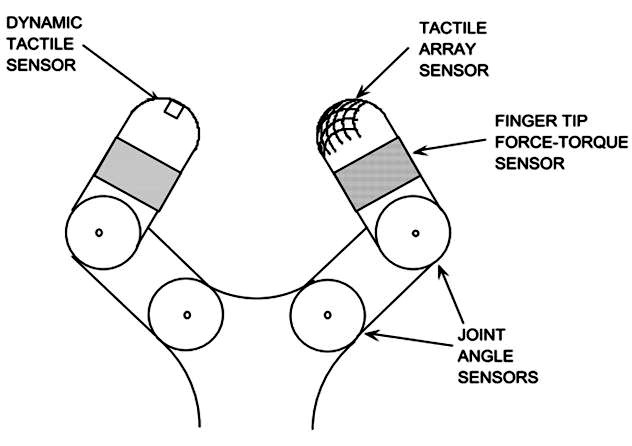
\includegraphics[width=\linewidth]{images/touch_sensors}
%	\caption{Schematic drawing of a robot hand with several types of contact sensors, reproduced from~\cite{howe1993tactile}. Permission to reproduce is pending.}
%	\label{fig:touch_sensors}
%\end{figure}
%ENDFIGURE

The authors in~\cite{leoni1998implementing} present an approach to tactile-motor coordination of a robotic hand based on a neurological model of the human tactile-motor system.
This model is implemented as a series of ANNs whose function and structure reflect discoveries in the human sensory areas specific to object grasping.
A scheme based on SOMs was chosen to model these sensory areas, since they must process a high rate of combined tactile and somatosensory input.
Use of the SOM controlled the volume of incoming inputs by making small, efficient adjustments to the model each time a new input vector became available.
%See Figure~\ref{fig:sensor_processing} for a graphical overview of their overall system.

The authors in~\cite{romano2011human} developed a human-inspired robotic grasp controller that gently picks up and sets down unknown objects.
They employ pressure sensors and accelerometers to mimic SA-I, FA-I and FA-II tactile channels (see Section~\ref{touch_sensing}).
An FSM is programmed to transition between six discrete states: (1) Close, (2) Load, (3) Lift and Hold, (4) Replace, (5) Unload, and (6) Open.
Transitions are based entirely on tactile event cues.
Their controller also dynamically adapts its initial grasp force depending on tactile events such as slipping, and judges when to set down the object in light of detected contact events with the table.

In~\cite{sikka1994tactile}, a new tactile-based object manipulation strategy was proposed, called tactile servoing.
Analogous to vision-based visual servoing, each state in the manipulation task sequence is characterized by tactile images detected via tactile sensor arrays on the robot hand.
%An example of such a tactile image can be found in Figure~\ref{fig:tactile_input}.
The authors' conclusion was that tactile sensors are useful in simple, direct and effective control of robots during manipulation tasks.
The literature supports the fact that tactile data is processed much the same way that visual data is processed in the human brain~\cite{johansson2001eye, scilingo2004perception}.

\section{Sensory Information Processing}

%In this section, we present work on efficient processing of sensory input data, as collected during a robotic manipulation.

\subsection{Force and tactile sensing for robotic manipulation}

%FIGURE (1.3)
%\begin{figure}[]
%	\centering
%	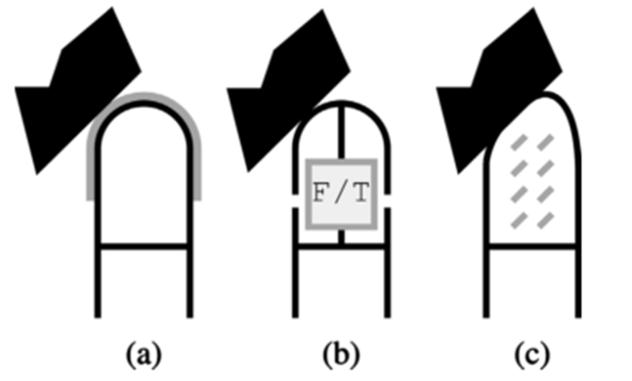
\includegraphics[width=\linewidth]{images/fingertip_sensors}
%	\caption{Different fingertip sensors: (a) tactile array - extrinsic; (b) force/torque sensor - intrinsic; and (c) fluid-filled~\cite{dasu2006information}.}
%	\label{fig:fingertip_sensors}
%\end{figure}
%%ENDFIGURE

Force and tactile sensing can provide information about mechanical properties, such as compliance, coefficient of friction, and mass, which are not perceivable through other means (e.g. vision)~\cite{howe1993tactile}.
Obtaining object properties via force and tactile sensing for the purposes of succeeding in manipulation tasks has been the subject of numerous studies~\cite{Heidemann2004, Detry2011, lepora2012embodied}.

The application of force and tactile sensors to many robotics problems affords new solutions that have previously been intractable via traditional, often computer vision-based methods~\cite{lee1999review}.
In their 2005 review article, Tegin and Wikander~\cite{tegin2005tactile} stress that, in contrast to the amount of literature on the application of vision-based solutions to robotics problems, literature on exploiting contact information (e.g. tactile) remains relatively rare.
One reason may be simply due to the lack of availability of force and tactile sensors in comparison to cameras~\cite{howe1993tactile}.

While vision is arguably the dominant sense in primates, including humans, there are certain scenarios in which vision fails, such as during object occlusion or when sensory resolution is too low for a given task.
In such cases, more detailed and versatile contact information may compensate for these deficiencies.

In~\cite{cutkosky2008force} the authors review techniques for processing and combining force and tactile information to develop abstract understanding of a given manipulation.
%present various layers of processing that transform raw force and tactile-sensor inputs into abstract understanding of an environment, such as object shape and contact types.
An excerpt of these processing techniques is shown graphically in Figure~\ref{fig:touch_id}: as raw sensory data travels from left to right, they are processed and combined to provide increasingly abstract understanding of a manipulation.
The authors state that force and tactile sensors have potential to yield the following information:
(1) object contact/no contact; 
(2) contact configuration (surface, edge, point, etc.) based on pressure-patterns; 
(3) object slip via vibrations in the grasped object, 
(4) properties (compliance, texture, friction, etc.) of an object via haptic exploration; and 
(5) feedback for control.
Given the above information, a robot can more appropriately control the force and moment on an object to accomplish the desired manipulation task.

%For object exploration, information such as local geometry, hardness, friction, texture, etc. must be obtained and integrated.
%In order to respond to events, the type and magnitude of events enacted, by for example an external agent, must be detected and properly assessed.

\subsubsection*{Example}

\begin{figure}[]
	\centering
	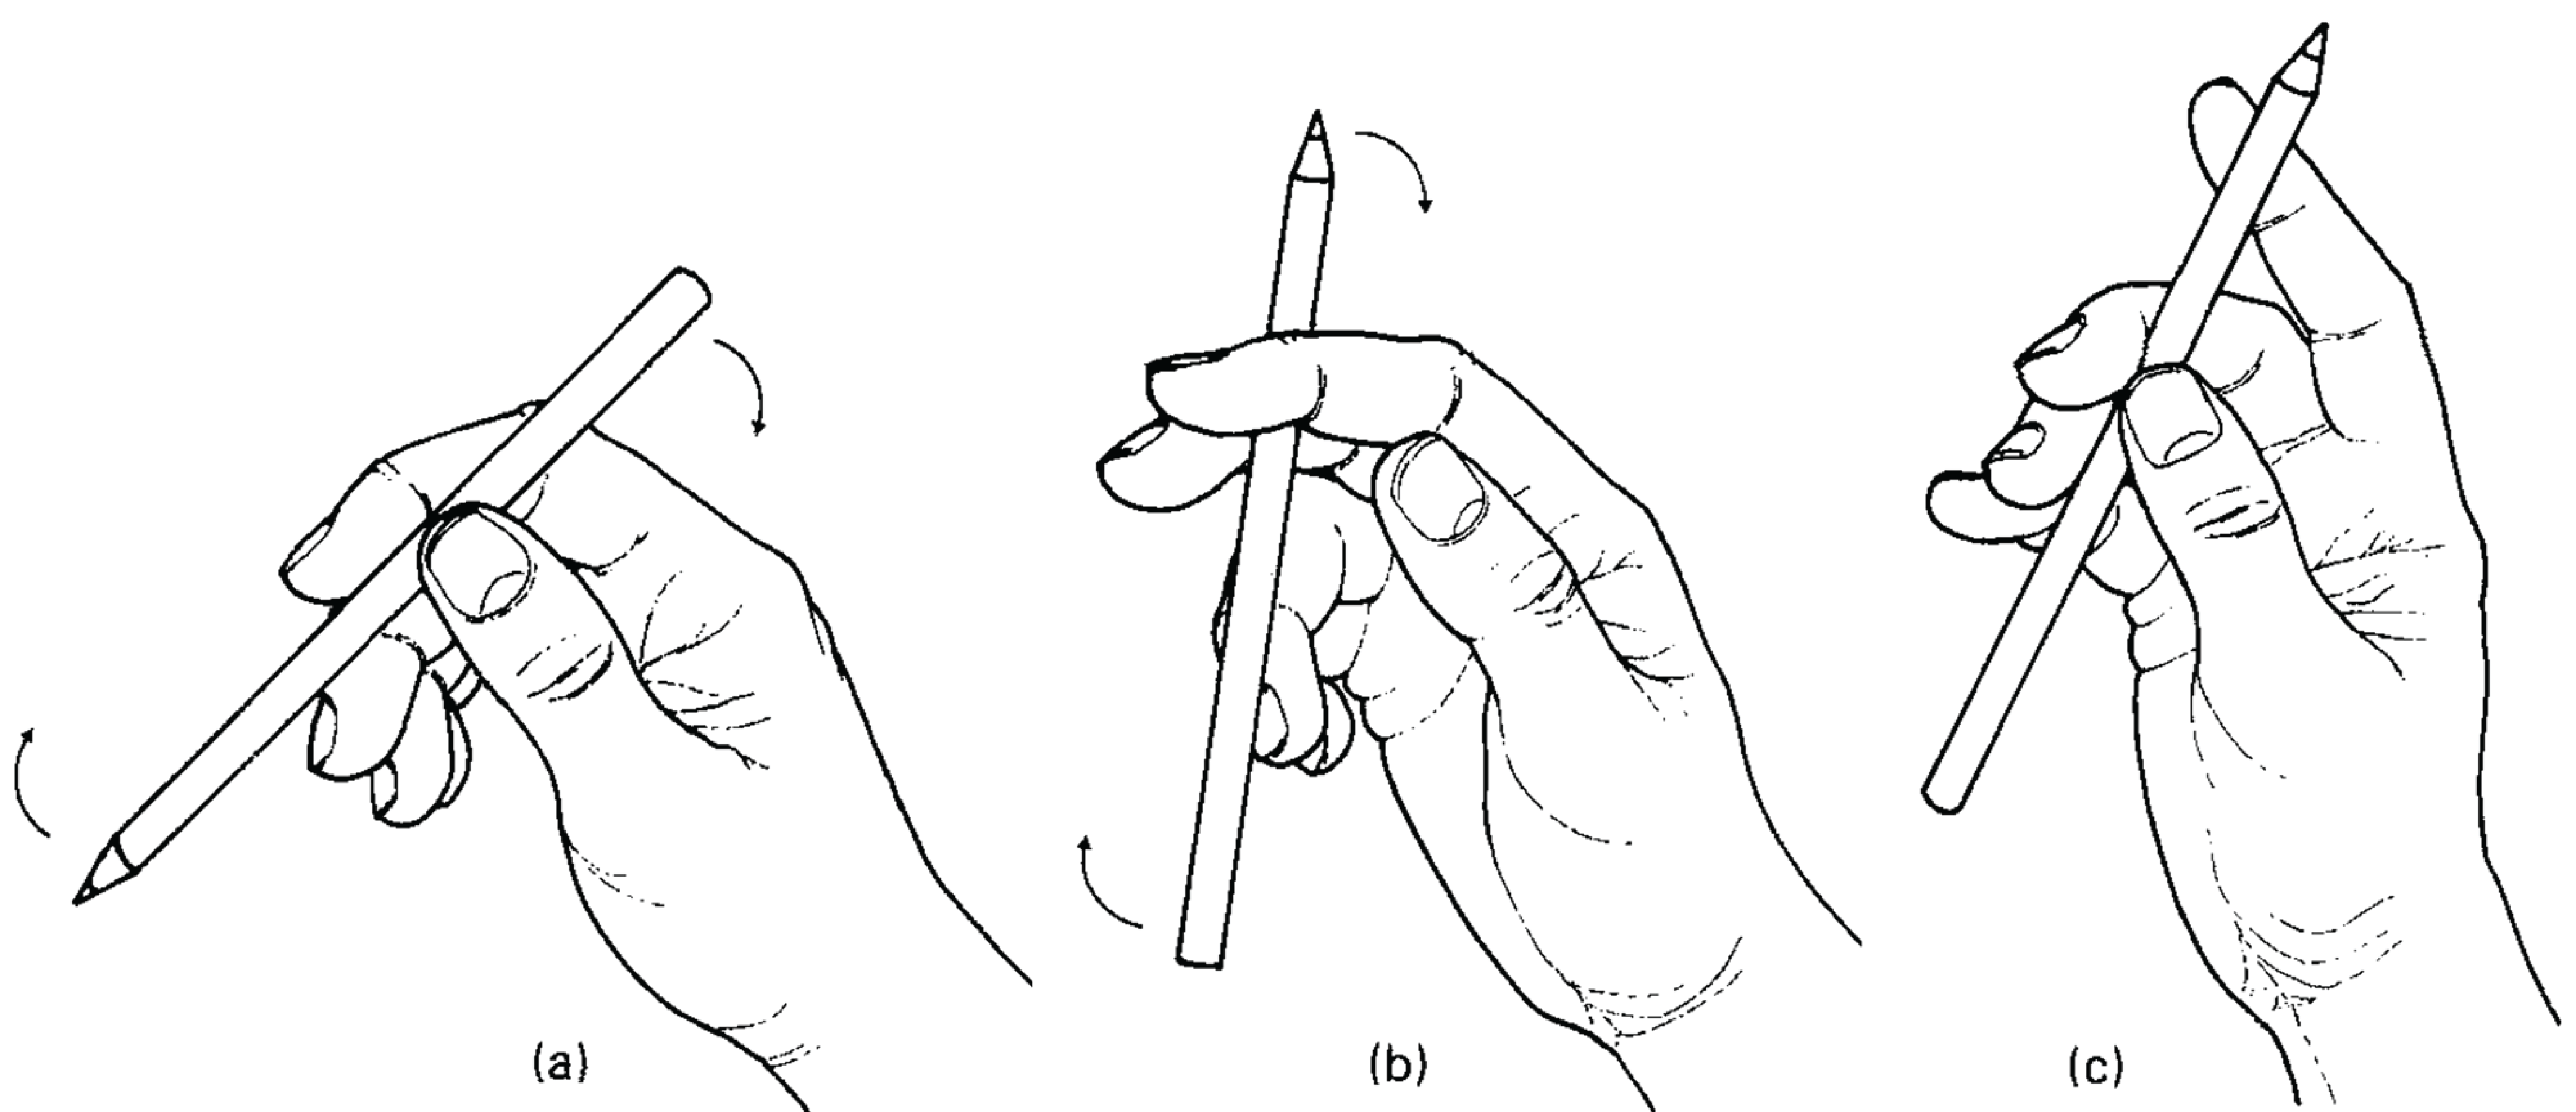
\includegraphics[width=\linewidth]{images/pen_twirling}
	\caption{Schematic drawing of the pen-twirling task. Drawings reproduced from~\cite{elliott1984classification}. Use of the reproduction is by permission of the copyright owner, John Wiley and Sons.}
	\label{fig:pen_twirling}
\end{figure}

Consider the following example: how might one accomplish the task of twirling a pen end-over-end between one's fingers, as demonstrated in Figure~\ref{fig:pen_twirling}? 
%What information would one use?  
The position and orientation of the object must somehow match imposed forces to maintain stability.
Successfully tracking the movement of the pen requires the knowledge of many variables, such as the configuration of one's hand, the locations and movements of contacts between the pen and one's fingers, the magnitudes of grasp forces, the contact conditions with respect to friction limits, etc.
How is it that, with enough practice, one can control all of these parameters effortlessly, even in the absense of visual feedback? 

A potential answer can be seen in Figure~\ref{fig:touch_id}: we can combine the forward kinematic model of the hand together with current finger joint angles to determine the positions and orientations of the finger tips.
When combined with force/torque measurements at the points of contact, it is possible to obtain local information of object shape, surface normal orientation, etc., which could then be combined to track the geometric pose of the object.

%Figure 2.8: 
\begin{figure}[]
	\centering
	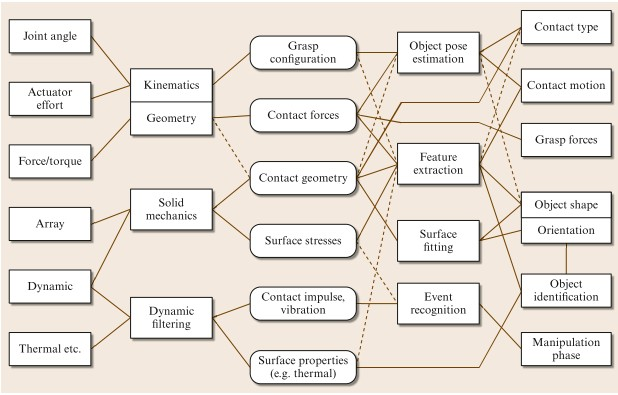
\includegraphics[width=\linewidth]{images/touch_id}
	\caption{Force and tactile sensor processing to estimate object pose~\cite{cutkosky2008force}.}
	\label{fig:touch_id}
\end{figure}
%ENDFIGURE

\subsubsection*{Tactile sensing}

For robotic hands with tactile sensor arrays, such as the BarrettHand, curvature and shape information can be obtained by measuring the local curvature at each element of the sensor array~\cite{cutkosky2008force}.
From there, it is possible to extract features, such as corners and edges of the object by combining local shape information from multiple sensors.
This task can be greatly enhanced if at least a partial model of the grasped object is available apriori, in which case the object can be statistically matched via surface or data fitting methods~\cite{fearing1990tactile}.

The most common application of tactile information has been to classify and recognize objects from a known set based on calculated geometric information of the object from raw tactile data.
Features, such as holes, edges and corners~\cite{cutkosky2008force} and object surfaces~\cite{overton1981tactile} have been used and extracted from tactile array, force and/or joint sensor information.
For example, Siegel~\cite{siegel1991finding} devised a way to extract object pose of a known object in a robot's grasp via joint angle and joint torque measurements.

\subsubsection*{Active sensing}
%The common solution to obtaining object properties via force and tactile sensing is to use carefully-tailored exploratory procedures that allow the desired properties to be easily and directly predicted from the gathered data~\cite{ruiz2010prediction}.
Since force and tactile sensors provide only local object information, recognition and disambiguation often require the hand to actively explore multiple areas of the object surface.
These types of strategies are referred to as active sensing.
There exist many example applications of active sensing, such as tracing object contours, measuring compliance and determining lateral extent of object surfaces.
In~\cite{muthukrishnan1987edge}, the authors propose an active sensing strategy to edge-finding by exploring the surface of an object until contiguous segments of tactile array impressions are found.
In~\cite{lepora2012embodied}, tactile sensors are used to discriminate shape and position of various textured cylindrical objects.
In~\cite{Detry2011}, grasp affordances are obtained through exploration of the pose space of manipulable objects. 

\subsubsection*{Dynamic sensing}

The ability to detect tactile events with respect to time (e.g. object slip) is important to many manipulation tasks such as lifting fragile objects.
The challenge lies in detecting such events reliably in the presence of sensor noise.
Highly sensitive tactile sensors capable of detecting minute events can be easily thrown off by e.g. vibrations from the robot actuators or by rapid robot acceleration.
Robust dynamic event detection can be solved by comparing tactile sensor readings at and away from contact regions, or even more robustly via statistical pattern matching methods that detect the signature of particular dynamic events~\cite{tremblay1993estimating}.



%TODO: FROM PAPER

\subsection{Anomaly detection in streaming data}

Since high-dimensional data streams often exhibit considerable structure, information that does not fit within this structure is most likely an anomaly, or outlier, in comparison to the vast majority of other input data.
An anomaly can be defined as an event or pattern which does not conform to some well-defined notion of normal phenomena.
Detecting the existence of anomalies within data streams is an important topic within both the data mining and machine learning communities~\cite{aggarwal2003framework,kifer2004detecting,dasu2006information,yamanishi2002unifying,song2007statistical} and has far-reaching applications in such areas as fault detection, fraud detection, sensor-networks and image processing~\cite{Chandola2009}.
In~\cite{hornung2014anomaly}, a model-free approach is taken to find anomalies in high-dimensional sensory streams. Data collected from the robot are first passed through a PCA-based feature extractor before building models of normal operation.

%Our framework develops a model of the sensory data over the course of a prescribed motion and therefore our system can detect anomalies as data points that are in poor correspondence with predicted values.
%Knowledge of this anomaly can then initiate further action such as autonomous adaptation to cope with this anomaly or updating the current model to explain this anomaly and therefore better reflect reality.

\subsection{Dimensionality reduction}

As the number of sensors available to a system increase, the computational, storage and transmission costs in inferring information from all available sensor readings also increase.
Therefore, given a large number of sensor readings, it is important to develop a reduced set of measurements or derived features that can model desired information in a compact fashion.  
Dimensionality reduction techniques can be classified into two broad categories: (1) feature extraction and (2) feature selection.  Most feature \emph{extraction} techniques take an unsupervised~\cite{ghahramani1996algorithm,saul2003think,tenenbaum2000global,hein2010unsupervised} or self-supervised~\cite{angelova2007dimensionality,dahlkamp2006self,lieb2005adaptive,sofman2006improving} learning approach.  
The result is a transformed, lower-dimensional set of features that more compactly describe the underlying structure of the data.  
In contrast, feature \emph{selection} techniques, such as those based on feature similarity~\cite{mitra2002unsupervised} and genetic algorithms~\cite{huang2006ga}, achieve dimensionality reduction by considering only a subset of input dimensions. 
In~\cite{pais2013learning}, the authors present a novel feature selection method comparing the variance of sensor readings to choose to encode either force or position information while recording user-demonstrated trajectories.

%%FIGURE (2.2)
%\begin{figure}[]
%	\centering
%	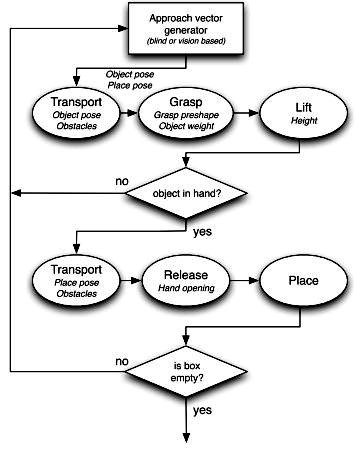
\includegraphics[width=\linewidth]{images/grasp_fsm}
%	\caption{Discrete states and transition conditions in the finite state machine that defines the empty-the-box manipulation task~\cite{felip2011emptying}.}
%	\label{fig:grasp_fsm}
%\end{figure}
%%ENDFIGURE

%%Figure 2.3: 
%\begin{figure}[]
%	\centering
%	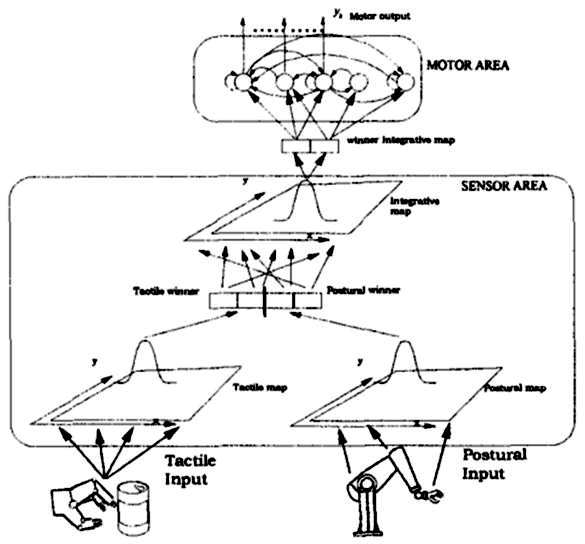
\includegraphics[width=\linewidth]{images/sensor_processing}
%	\caption{Structure of ANNs chosen by the authors as a model for human grasping~\cite{leoni1998implementing}.}
%	\label{fig:sensor_processing}
%\end{figure}
%%ENDFIGURE

%%Figure 2.4: 
%\begin{figure}[]
%	\centering
%	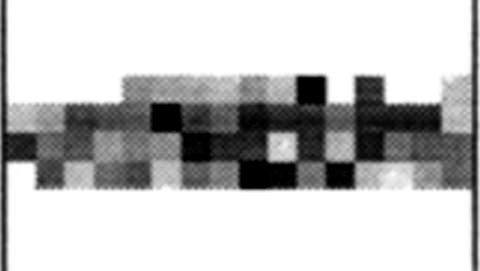
\includegraphics[width=\linewidth]{images/tactile_input}
%	\caption{Example tactile image during the rolling-pin task by planar robot finger equipped with tactile sensor array in~\cite{sikka1994tactile}.
%Darkness indicates pressure intensity.}
%	\label{fig:tactile_input}
%\end{figure}
%%ENDFIGURE

%%Figure 2.5: 
%\begin{figure}[]
%	\centering
%	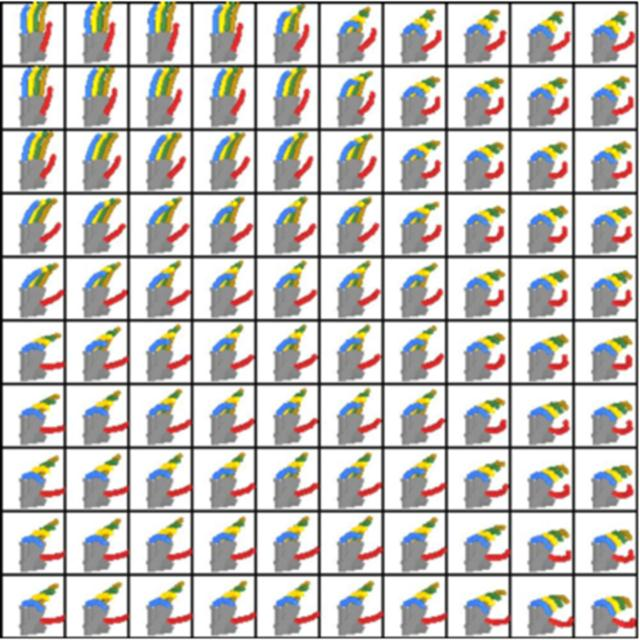
\includegraphics[width=\linewidth]{images/grasp_som}
%	\caption{Discrete grasp manifold of successful grasps based on the SOM.
%Note how similar grasp postures are organized together which results in fast queries of the experience base~\cite{steffen2007experience}.}
%	\label{fig:grasp_som}
%\end{figure}
%%ENDFIGURE
%
%%FIGURE (1.8)
%\begin{figure}[]
%	\centering
%	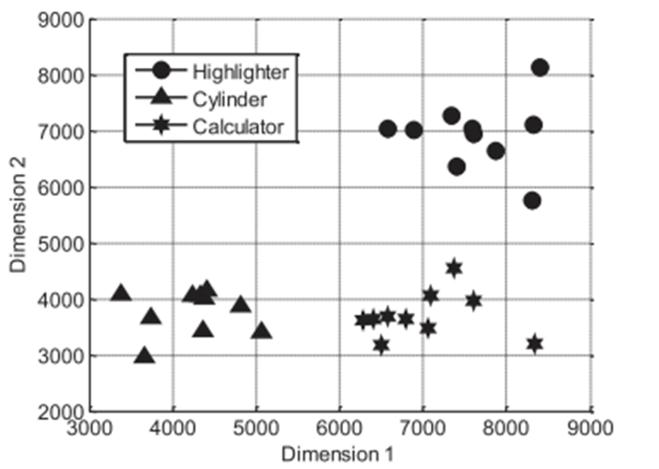
\includegraphics[width=\linewidth]{images/sensory_clustering}
%	\caption{Clusters of outputs from trained spiking neural network for certain objects~\cite{ratnasingam2011spiking}.}
%	\label{fig:sensory_clustering}
%\end{figure}
%%ENDFIGURE

%%FIGURE (1.9, 2.7)
%\begin{figure}[]
%	\centering
%	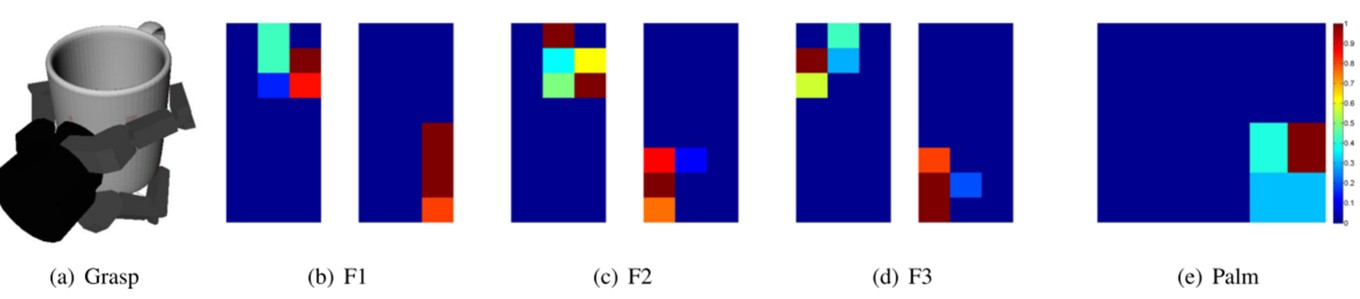
\includegraphics[width=\linewidth]{images/grasp_tactile_example}
%	\caption{Example grasp feature vector in successful grasp database: (a) shows the kinematic state of the grasp around the object, (b) (c) (d) and (e) represent the tactile feedback experienced by the first, second, third fingers and palm of the BarrettHand respectively.}
%	\label{fig:tact_example}
%\end{figure}
%%ENDFIGURE


%%FIGURE (?, 2.8)
%\begin{figure}[]
%	\centering
%	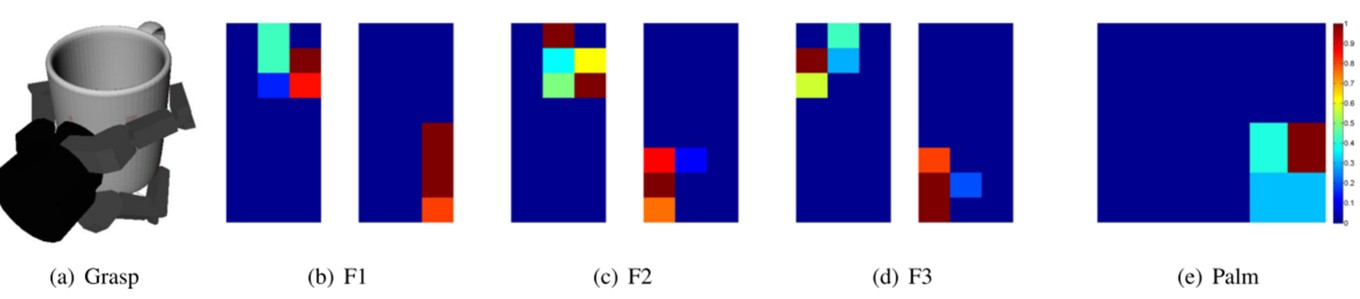
\includegraphics[width=\linewidth]{images/grasp_tactile_example}
%	\caption{Example grasp feature vector in successful grasp database: (a) shows the kinematic state of the grasp around the object, (b) (c) (d) and (e) represent the tactile feedback experienced by the first, second, third fingers and palm of the BarrettHand respectively~\cite{dang2011blind}.}
%	\label{fig:tact_example}
%\end{figure}
%%ENDFIGURE

\begin{landscape}
%FIGURE (2.11, 2.12)
\begin{figure}
    %\begin{subfigure}[]{0.515\linewidth}
    %    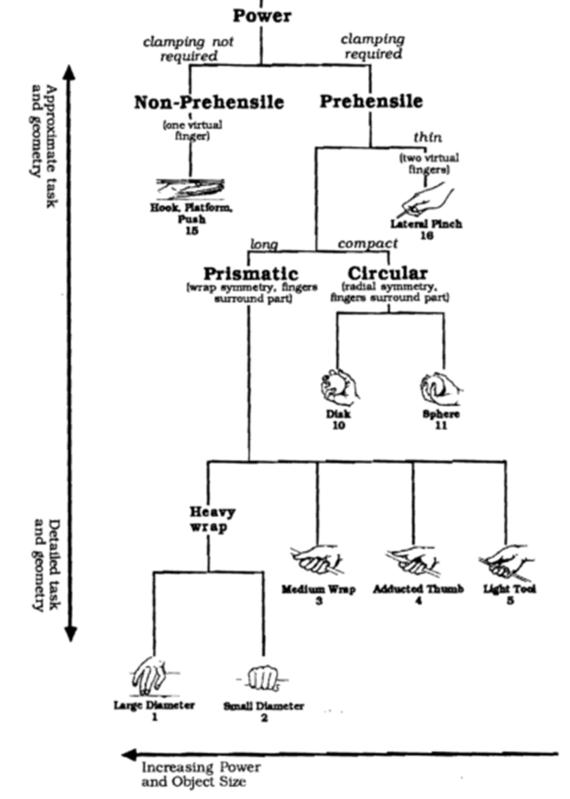
\includegraphics[width=\linewidth]{images/power_grasps}
    %    \caption{Taxonomy of power manipulation skills~\cite{howe1993tactile}.}
    %    \label{fig:power_taxonomy}
    %\end{subfigure}
    %\begin{subfigure}[]{0.485\linewidth}
    %    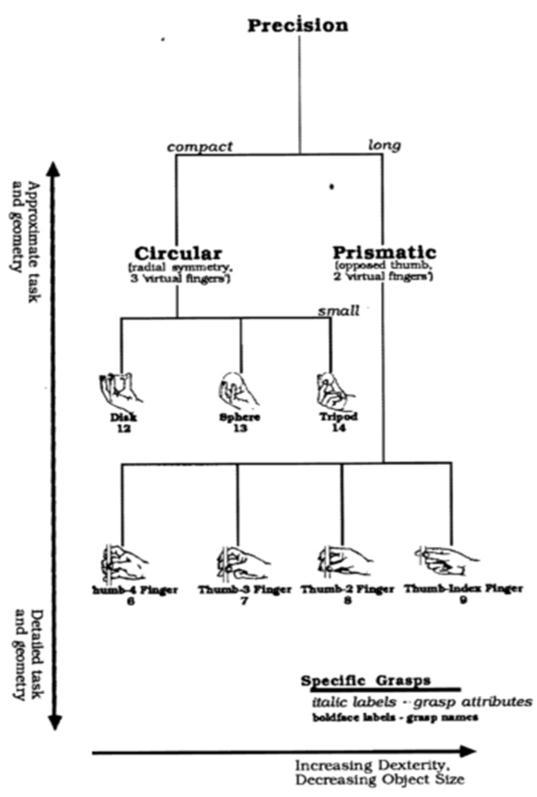
\includegraphics[width=\linewidth]{images/precision_grasps}
    %    \caption{Taxonomy of precision manipulation skills~\cite{howe1993tactile}.}
    %    \label{fig:precision_taxonomy}
    %\end{subfigure}
    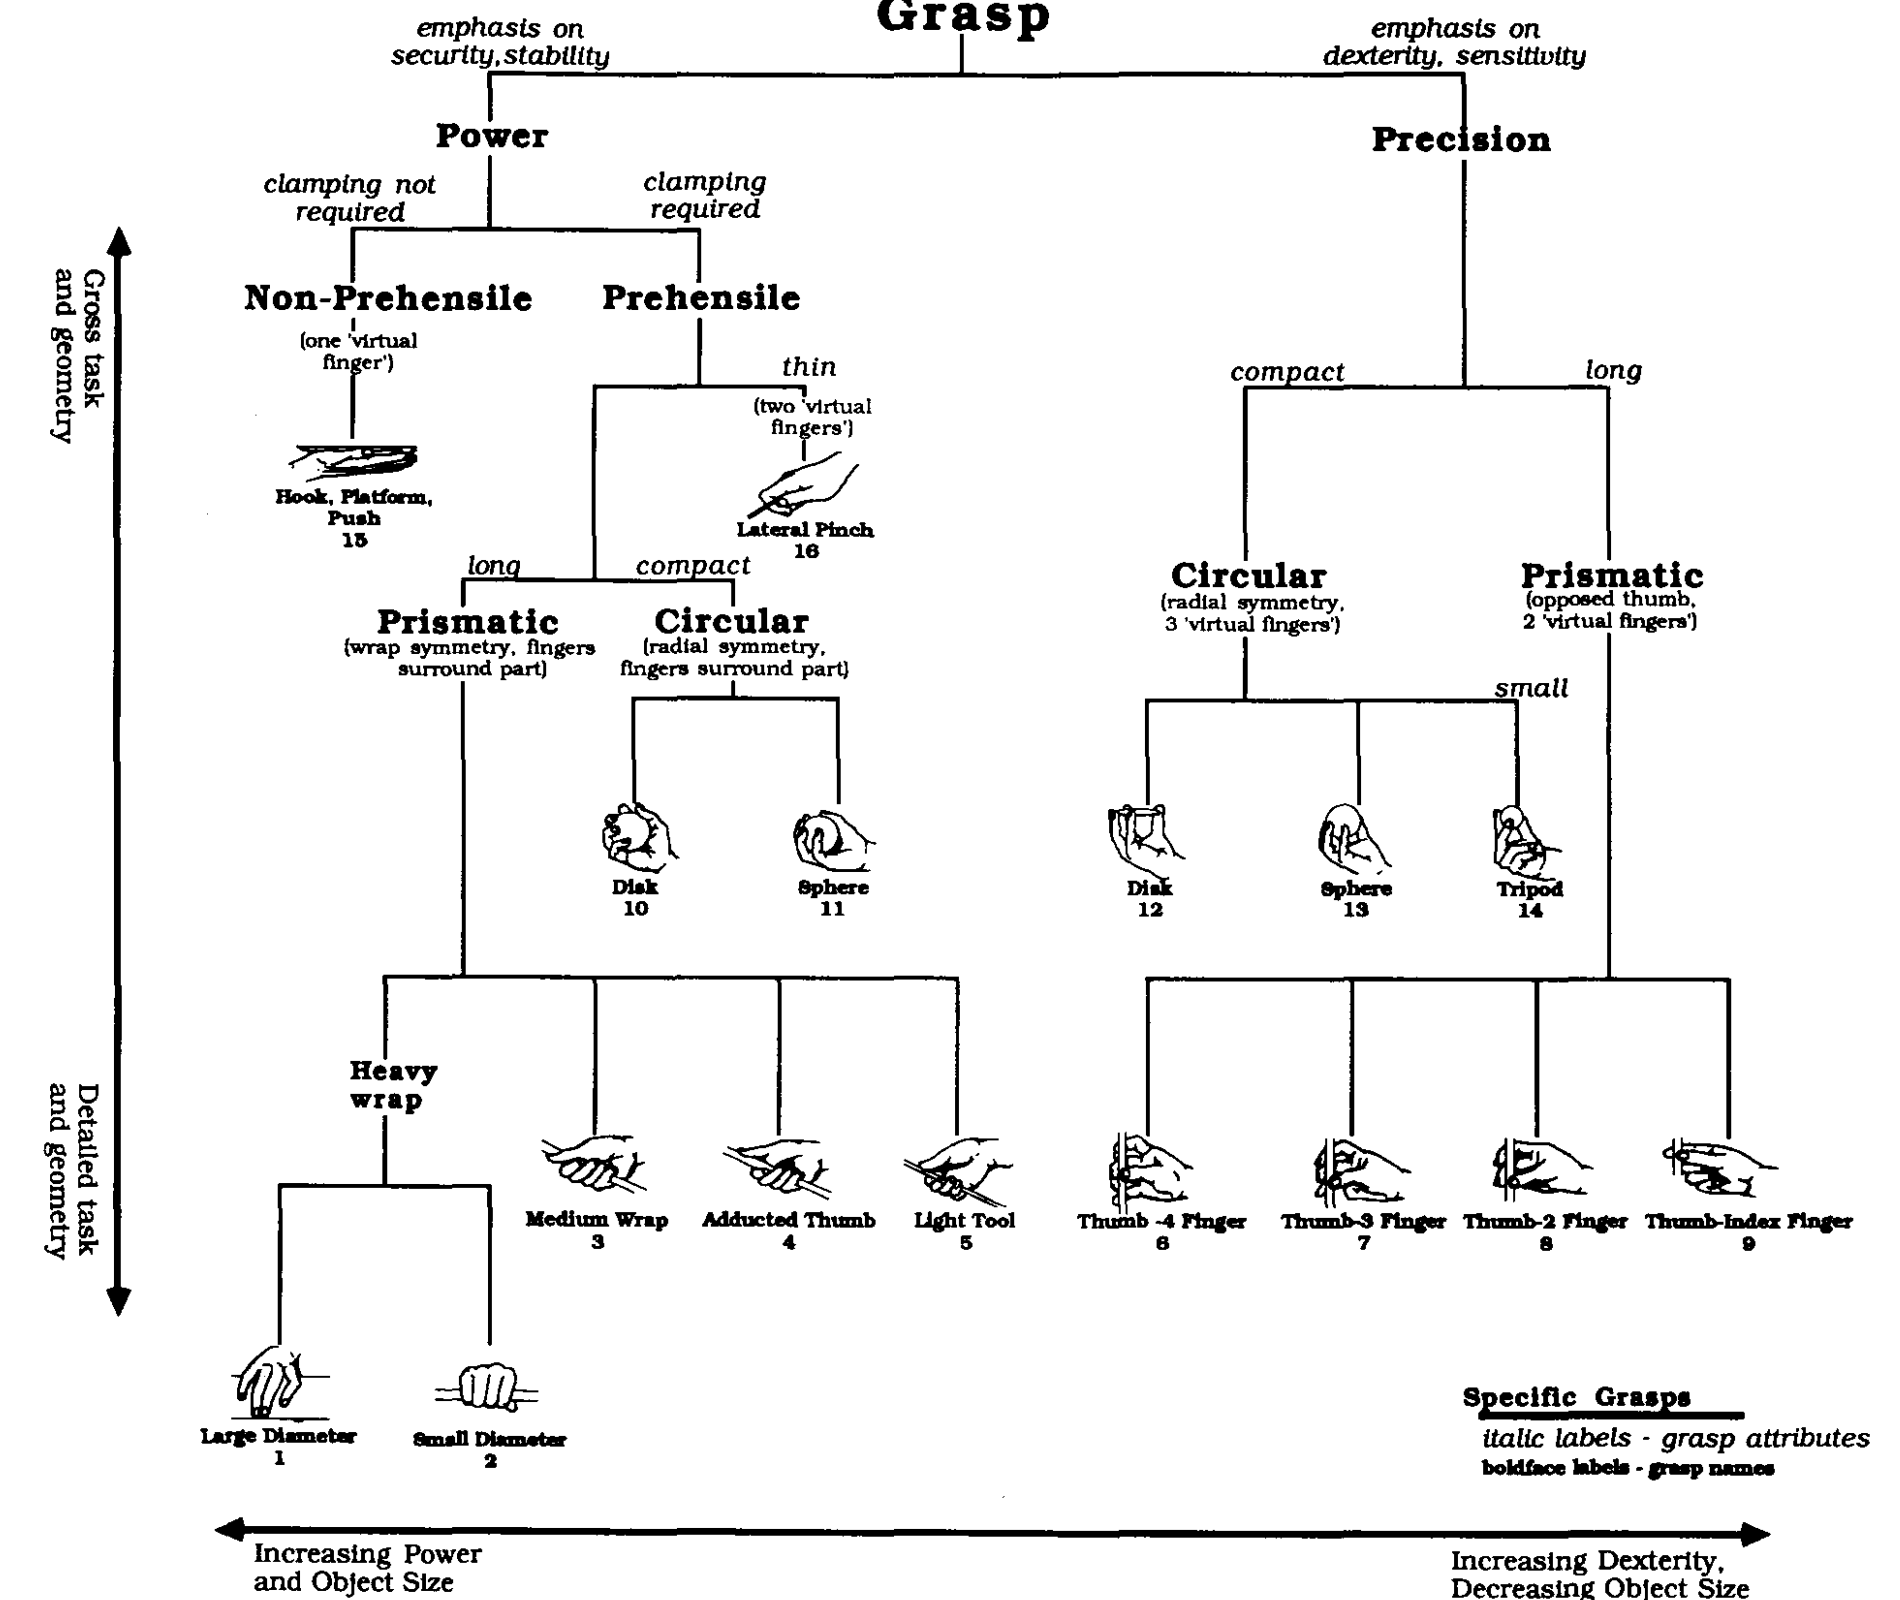
\includegraphics[width=\linewidth]{images/grasp_dichotomy}
    \caption{Dichotomy of human grasping, reproduced from~\cite{cutkosky1989grasp}. \copyright 1989 IEEE. }
%Non-prehensile grasping uses gravity as a means of securing the object to the hand.
    \label{fig:grasp_dichotomy}
\end{figure}
%ENDFIGURE
\end{landscape}

\section{Neuroscience \& Physiology}

%\begin{figure}[]
%	\centering
%	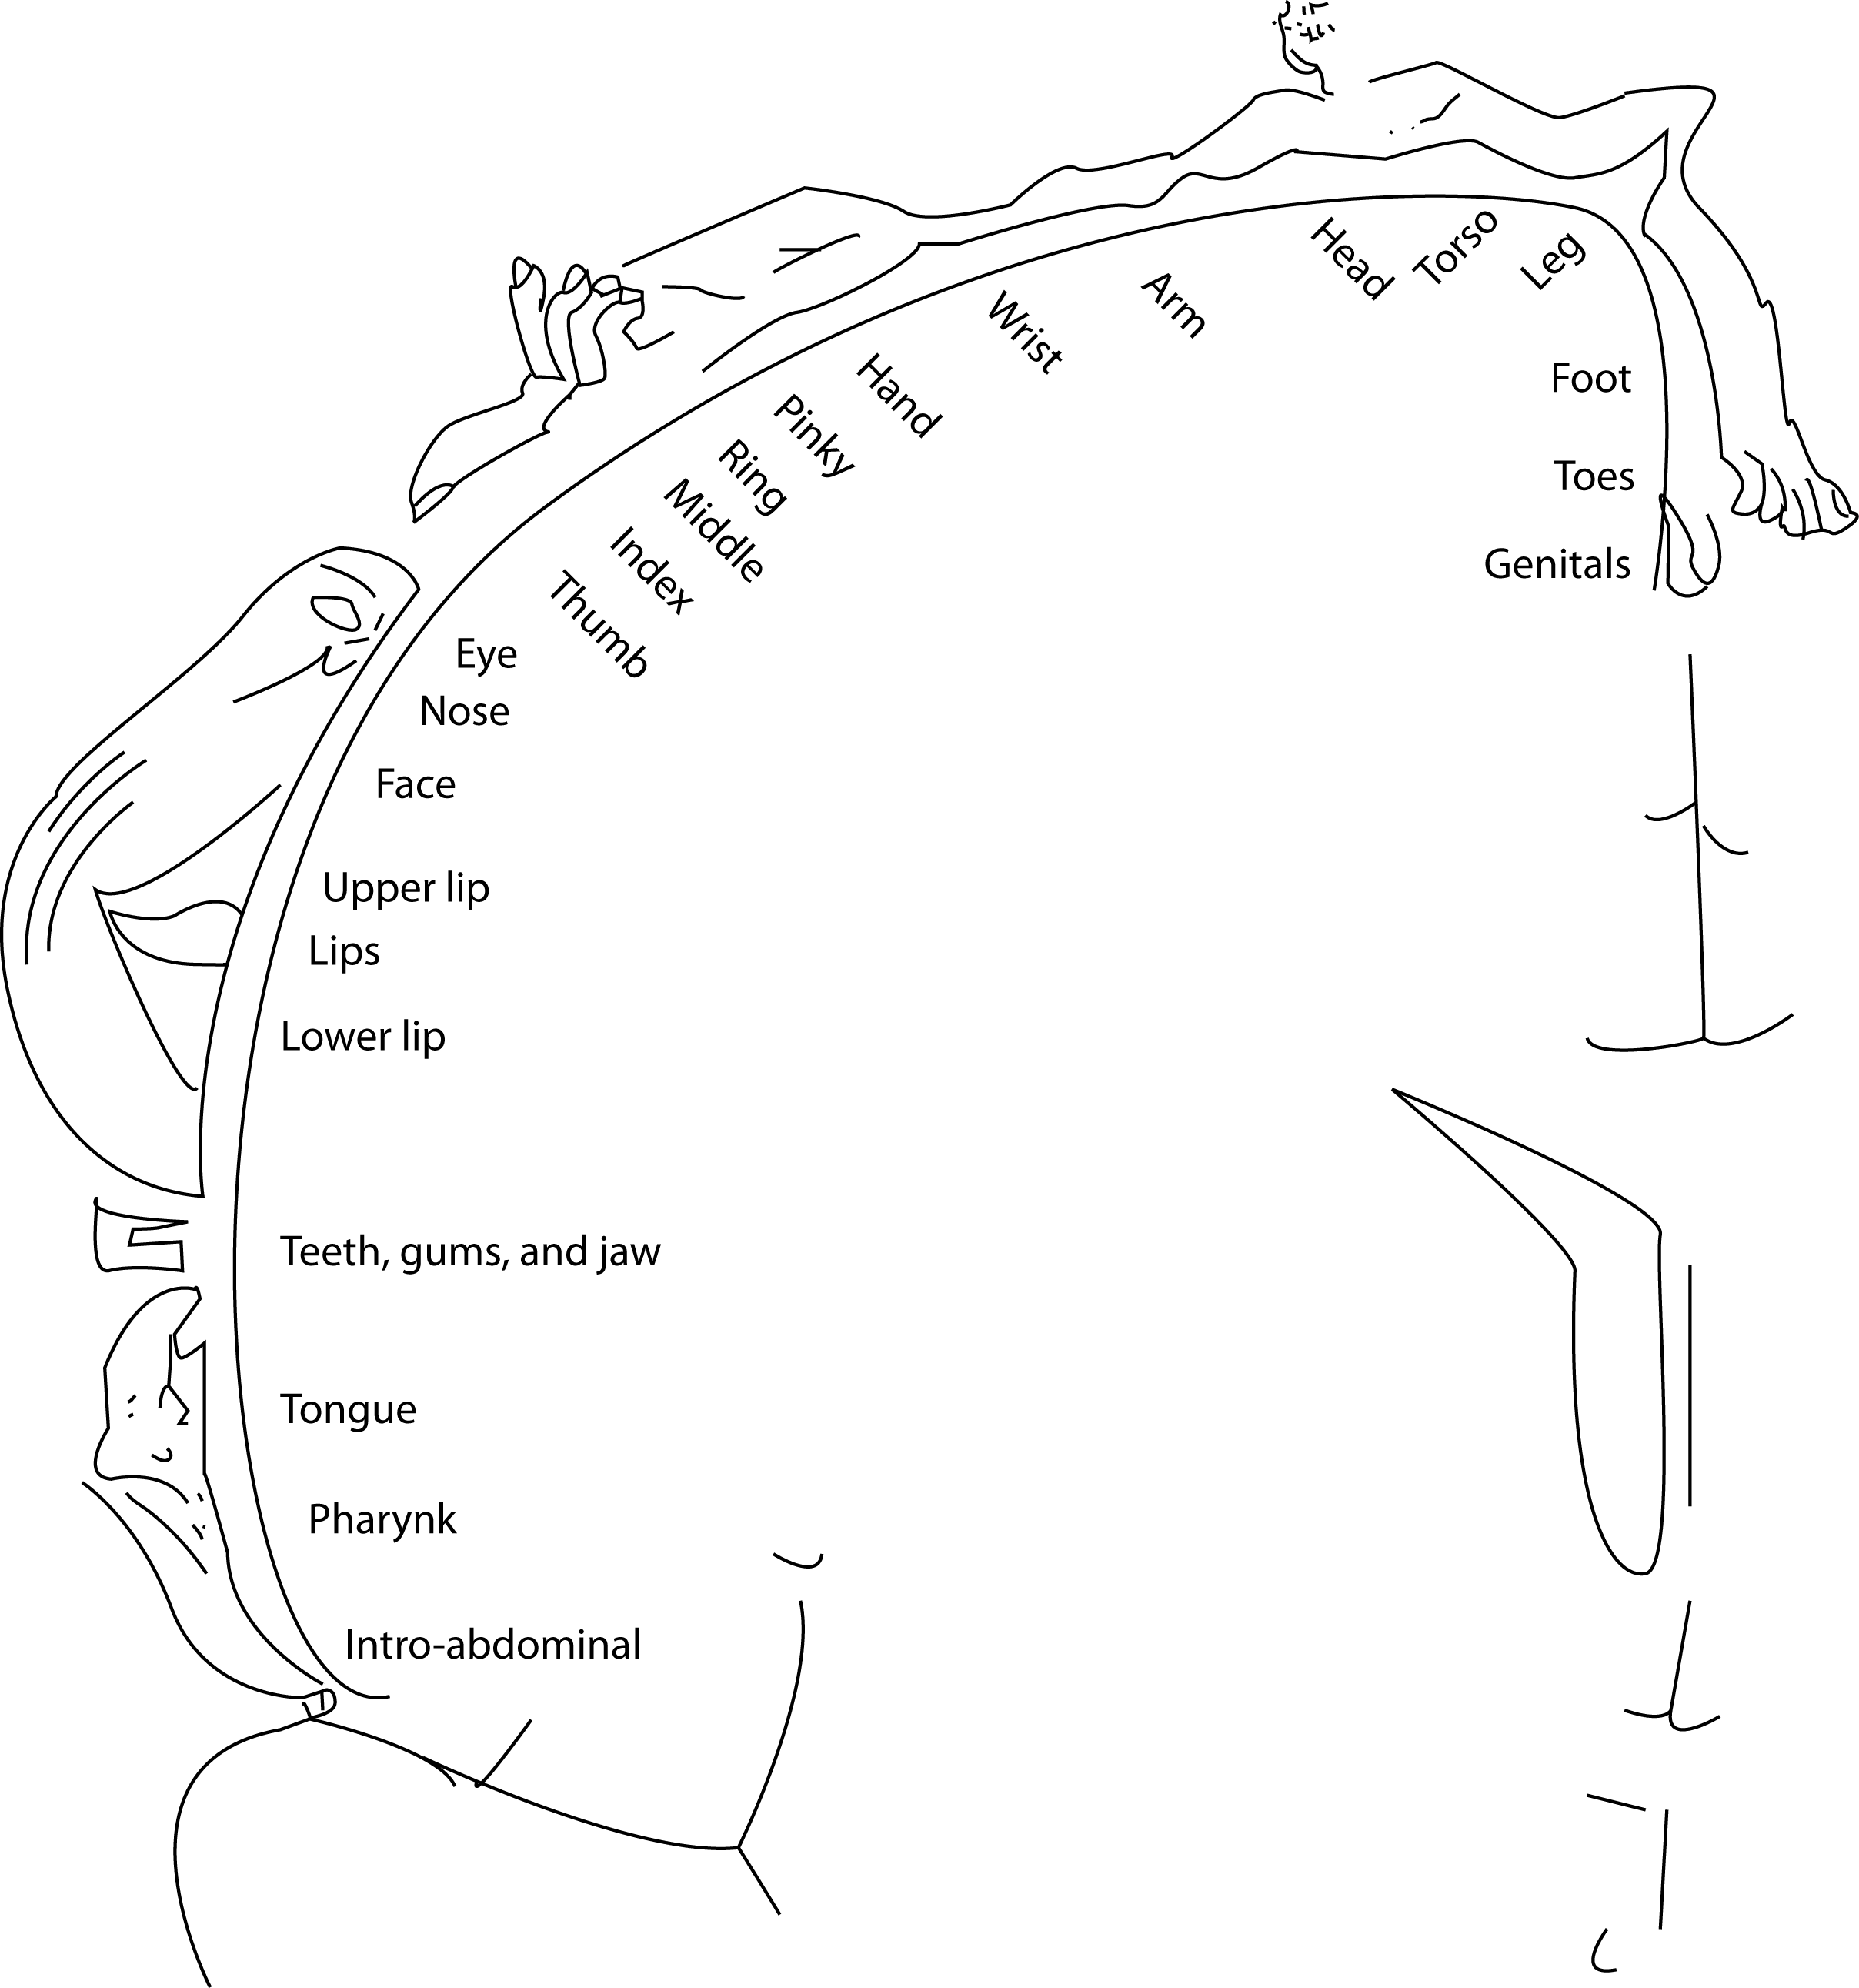
\includegraphics[width=\linewidth]{images/sensory_homunculus_penfield}
%	\caption{Human Cortical Homunculus of Penfield and Rasmussen, reproduced from~\cite{penfield1950cerebral}. Permission to reproduce is pending.}
%	\label{fig:sensory_homunculus_penfield}
%\end{figure}

Studying the manipulation capabilities of humans and animals for the purpose of designing better robotic systems is a challenge.
First, it is hard to discover the precise algorithms that our brains employ.
Second, the mechanics of the human hand is highly complex and thus the algorithms our motor system employs may not be appropriate for the relatively simple mechanics of a robot.
Nevertheless, studying human manipulation can provide insight into designing more efficient and effective robotic systems.
In this section, we attempt to draw such insight by exploring the human motor system as presented in a sample of the neuroscience and physiology literature.

\subsection{Object manipulation: definitions}

In this section, we present some common vocabulary used by researchers in describing object manipulation tasks as performed by humans.

\subsubsection*{The power-precision dichotomy}

Humans employ a wide variety of manipulation skills depending on the object being manipulated.
When opening a jar, for example, a power-style grip is required to loosen the jar.
Once the lid is loose and required torque is lessened, a lighter grip is adopted for speed and precision.
This dichotomy of power/precision prehensile (i.e. grasping) activities was proposed by Napier in 1956~\cite{napier1956prehensile}.
Figure~\ref{fig:tie_rope} provides an example of these two patterns of activity in the manipulation task of tying a knot: power is required to hold the rope in place while precision is required to tie the knot. 
Cutkosky and Wright also propose a taxonomy of human grasps in~\cite{cutkosky1989grasp}, breaking down the dichotomy of power/precision even further (see Figure~\ref{fig:grasp_dichotomy}).
Depending on the weight and size of the object as well as the desired dexterity of the hand, a human adopts a different style of grip.

%FIGURE (2.10)
\begin{figure}[]
	\centering
	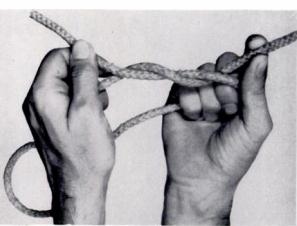
\includegraphics[width=\linewidth]{images/tie_rope}
	\caption{Tying a knot: manipulation task combining precision and power grips. Figure inspired by~\cite{napier1956prehensile}.}
	\label{fig:tie_rope}
\end{figure}
%ENDFIGURE


\subsubsection*{Analytical measures of grasp quality}
The authors in~\cite{cutkosky1990human} present common measures of grasp quality, which may be optimized or become part of the set of constraints with respect to a given manipulation task.
An overview of these analytical grasp-quality measures is presented in Table~\ref{tbl:grasp_metrics}.
The set of ideal grasps of any object then exists within the space of grasps that satisfy all hard constraints and optimize important soft constraints with respect to the given task.
For example, Nakamura et al. search for grasps that minimize internal forces (i.e. grasping effort), subject to constraints on force closure and manipulability~\cite{nakamura1987mechanics}.
According to physiological findings, humans tend to employ a similar scheme as proposed by Nakamura et al. where a certain frictional safety margin is maintained~\cite{ring1968paper}.

Human grasps have also been studied in terms of these analytical measures.
For example, power grasps can be thought of as having higher compliance, stability and slip resistance than precision grasps.
Power grasps also tend to have a connectivity of zero (since the fingers do not play a manipulating role).
In contrast, precision grasps have high manipulability and connectivity (of at least three and often six)~\cite{cutkosky1990human}.

\begin{table}[h]
\begin{tabular}{rl}
\textbf{Metric}                       & \textbf{Description}                                                               \\ \hline
\multicolumn{1}{|r|}{Compliance}      & \multicolumn{1}{l|}{Inverse-stiffness of the object with respect to the hand}      \\ \hline
\multicolumn{1}{|r|}{Connectivity}    & \multicolumn{1}{l|}{Number of DOFs between grasped object and the hand}            \\ \hline
\multicolumn{1}{|r|}{Form closure}    & \multicolumn{1}{l|}{External forces are unable to unseat the grasped object}       \\ \hline
\multicolumn{1}{|r|}{Force closure}   & \multicolumn{1}{l|}{Object held without slipping (a.k.a. frictional form closure)} \\ \hline
\multicolumn{1}{|r|}{Grasp isotropy}  & \multicolumn{1}{l|}{Fingers are able to accurately apply force/moment to object}   \\ \hline
\multicolumn{1}{|r|}{Internal forces} & \multicolumn{1}{l|}{Kinds of internal grasp forces hand may apply to the object}   \\ \hline
\multicolumn{1}{|r|}{Manipulability}  & \multicolumn{1}{l|}{Fingers can impart arbitrary motions (i.e. connectivity = 6)}  \\ \hline
\multicolumn{1}{|r|}{Slip resistance} & \multicolumn{1}{l|}{Amount of force required before object starts to slip}         \\ \hline
\multicolumn{1}{|r|}{Stability}       & \multicolumn{1}{l|}{Tendency of grasped object to return to a spatial equilibrium} \\ \hline
\end{tabular}
\caption{Common analytical measures that may be optimized or become a part of grasp constraints~\cite{cutkosky1990human}.}
\label{tbl:grasp_metrics}
\end{table}

\subsubsection*{Force vs. form closure}
A subtle yet important distinction must also be made between force closure and form closure.
Only rarely do humans adopt complete form closure of objects.
Form closure refers to grasping without the use of friction whereas force closure uses friction to keep objects seated in the hand.
An object likely requiring form closure would be for example a wet bar of soap or a slinky.

\subsubsection*{Slipping vs. crushing threshold}
While adequately large grip forces must be maintained to keep the object within a force closure grasp, exceedingly large forces are also not desirable as they cause unnecessary fatigue on the hand and may even crush fragile objects~\cite{johansson1994grasp},~\cite{gorniak2010manipulation}.
Thus, grip force is constrained by both the slipping and crushing thresholds of objects (see Figure~\ref{fig:grip_crush_force} for some examples).

%Figure 2.11: 
\begin{figure}[]
	\centering
	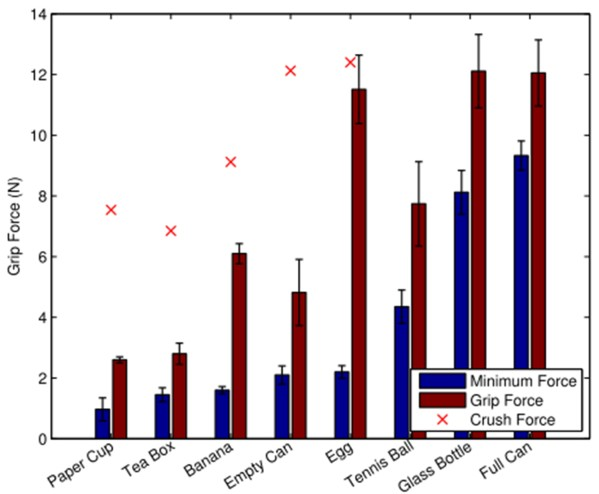
\includegraphics[width=\linewidth]{images/grip_crush_force}
	\caption{Example slipping and crushing thresholds of everyday objects. The difference between the required Minimum Force and observed Grip Force is known as the \emph{safety margin}. Data obtained from~\cite{romano2011human}.}
	\label{fig:grip_crush_force}
\end{figure}
%ENDFIGURE

The amount of force that subjects apply over and above the slipping threshold is known as the \emph{safety margin}.
The magnitude of the safety margin varies across subjects, and was found to be dependent on the dexterous manipulation skill of the subject in performing the given task~\cite{Johansson1984}.

When manipulating visually fragile objects, the initial force in human subjects is lighter and their action is slower when compared to manipulating visually non-fragile objects.
Once contact with the object is made, tactile feedback complements the missing information with respect to the true fragility of the object. 
Subjects can then properly carry out the planned action~\cite{chinellato2008visual}.
Accurate predictions are crucial however due to the relatively slow response rate of corrective actions~\cite{johansson2009coding}.

%Information on objects involved can be predicted as well.
%If grasp stability errors occur, real-time corrective actions are taken.

\subsection{Force and tactile sensing}
\label{touch_sensing}
The elements of the human sense of touch can be broken up into two distinct categories: proprioceptive and tactile.
Proprioceptive sensing refers to the perception of limb motion and forces using internal receptors, such as muscle spindles (responding to changes in muscle length), tendon organs (measuring muscle tension), and cutaneous afferents (reacting to skin deformations around the joints)~\cite{johansson2009coding}.
Proprioceptive receptors within the joints of the hand are also present, which report joint angles, forces and torques~\cite{howe1993tactile}.
Tactile sensing deals with the perception of contact information with receptors beneath the surface of the skin~\cite{vallbo1984properties}.

Actuation of the hand is imparted by muscles in the forearm through transmission of tension by tendons passing through the wrist.
It has been shown that due to dynamics of transmission such as friction, backlash, compliance and inertia, accurate control of endpoint position and forces based on proprioceptive signals alone is difficult~\cite{kaneko1991new}.
Thus, tactile afferents are essential for fine-grained mechanical measurements at contact locations~\cite{Johansson1984}.

Tactile afferents have received much attention in the physiology and neuroscience literature; a comprehensive summary of which may be found in~\cite{vallbo1984properties} and, more recently in~\cite{johansson2009coding}.
There are in total four specialized types of mechanoreceptive nerve endings within the skin of the human hand, each of which can be categorized as having large or small active areas (Type I and Type II respectively) and responding or not responding to static stimuli (SA for slowly adapting and FA for
fast adapting, respectively).
See Figure~\ref{fig:tactile_afferents} for a description of each of these types.
It has been calculated that a total of 17,000 specialized mechanoreceptors exist in the grasping surfaces of the human hand~\cite{johansson2009coding}.
In addition, there are free nerve endings that are sensitive to thermal and pain stimuli~\cite{howe1993tactile}.

%Figure 2.10: 
\begin{figure}[]
	\centering
	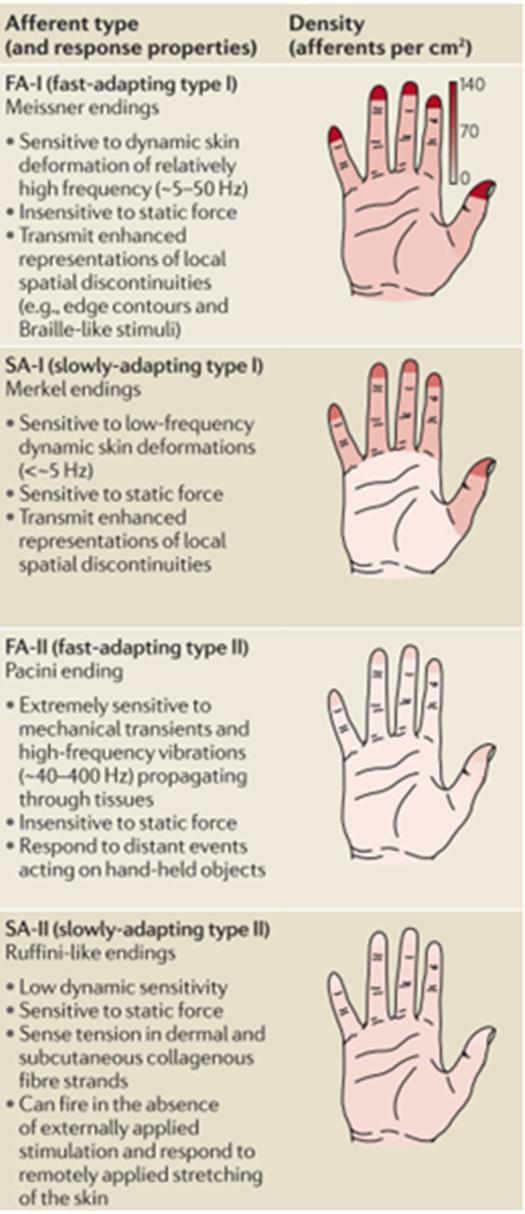
\includegraphics[width=0.7\textwidth]{images/tactile_afferents}
	\caption{Characteristic of tactile afferents within human fingertip skin.
Reproduced from~\cite{johansson2009coding}. Permission to reproduce granted by R.S. Johansson.}
	\label{fig:tactile_afferents}
\end{figure}
%ENDFIGURE

\subsection{High-level processes}
\label{high_level_processes}

In addition to low-level tactile and proprioceptive processing, the mammalian central nervous system performs many high-level processes such as prediction, planning and memory.
These processes support, guide, and organize our more primitive manipulative functions to accomplish more complex manipulation tasks.

\subsubsection*{Prediction}

In~\cite{johansson1994grasp}, the authors preclude that the magnitude of fingertip forces imposed on objects are determined by at least two high-level control processes: (1) anticipatory parameter control (APC) and (2) post-contact control.
The authors model APC as a feedforward controller that uses predictions of critical characteristics of the object (weight/friction/initial condition, etc.) based on the results of previous object manipulation experience.
Following contact with the object, sensory information can be extracted to (1) modify motor commands automatically; (2) update sensory memories for APC; (3) inform central nervous system of the completion of subgoals comprising a task; and (4) trigger subsequent subgoals.
The central nervous system monitors specific, expected events and produces control signals appropriate to each subgoal.
In contrast to feedback controllers, this feedforward, sensor-driven control strategy predicts appropriate control output several steps in advance.
Slips are avoided and force across digits is coordinated by independent control mechanisms based on local sensory information.

\subsubsection*{Planning}

Planning plays an important role in anticipating future events as well.
In~\cite{johansson2001eye}, Johansson, et al. demonstrate the importance of eye-hand coordination during manipulation tasks.
Subjects' gaze were tracked during a block-stacking task.
It was found that their gaze played an important role in planning each pick-and-place action.
The authors then further propose and demonstrate in~\cite{flanagan2003action} the direct matching hypothesis, which predicts that subjects will unconsciously produce eye movements when observing a familiar action as if they were performing the task themselves.
%This suggests deep coupling between gaze and object manipulation capabilities.

\subsubsection*{Supramodal processing}

In a study conducted by Bicchi et al.~\cite{scilingo2004perception}, it was found that the V5/MT cortex (the same area in the brain that responds to optical flow) is activated during tactile-flow perception, i.e. when dynamic movement is detected via tactile afferents.
This is consistent to other findings that there exists a supramodal, or multi-modal, organization of regions in the brain involved in both tactile-flow and optical-flow processing~\cite{flanagan2006control}.
In another study by Bicchi et al.~\cite{bicchi2003haptic}, it was found that certain experiments could fool the subjects' tactile flow processing in the brain through tactile illusions, much the same way that optical-flow processing can be fooled, which is known as the \emph{aperture problem}.

\subsubsection*{Action-phase control strategies}

Findings by Johansson et al. indicate that, during certain manipulation tasks, the human motor system functions as a sort of state machine that transitions based on sensory predictions and sensory inputs.
These states, or \emph{action-phases}, are defined as sequences of specific sensory events that are each linked to subgoals comprising a given task~\cite{johansson2009coding}.

Action-phase goals are evaluated by matching patterns in tactile afferent signals.
For example, grasp contact – a required action-phase subgoal for many manipulation tasks – detects patterns in SA-I and FA-II afferent inputs.
Combinations of certain afferents provide information such as contact timing, location, force intensity and direction.
Contact location is defined as the spatial center of all afferents involved in the overall signal.
Force intensity is characterized by the number of afferents involved as well as the firing rates of each.
Patterns of activity in combinations of afferents give us the direction of the detected contact force.

\subsubsection*{Dexterity}

Once a grasp is attained, adequate force within the friction cone of the object must be imposed to retain force closure.
Dexterity is then defined as the ability to adapt the balance of grip and load forces to object surface properties~\cite{howe1993tactile}.
Dexterous manipulation abilities are attributed mainly to tactile afferents since a loss in these abilities is experienced during digital anesthesia~\cite{Johansson1984}.

\subsubsection*{Object identification}

Tactile afferents during initial contact also provide object surface property information, which is frequently combined with visual cues and/or sensory memories to develop abstract understanding.
Reactions of FA-I, SA-I and SA-II afferents to object surface are used to determine object surface properties.
For example, FA-I afferents react more strongly to slippery surfaces~\cite{burstedt1997coordination}.

\subsubsection*{Filtering noise}

Robust processing of tactile afferent information is attributed to the brain's innate ability to detect coincidence: a phenomenon in which its central neurons receive synchronous input spikes from many distinct tactile afferents~\cite{hopfield1995pattern}.
Therefore, noise in the environment, i.e. information unrelated to the current focus of attention, can be characterized by input spikes which do not arrive at the brain at the same precise moment in time as input deemed valuable to the current task.





%\subsection{Non-prehensile manipulation} 
%
%This thesis is primarily concerned with non-prehensile manipulation tasks, as pioneered by Lynch and Mason~\cite{lynch1999dynamic}. 
%Non-prehensile manipulation has seen relatively little attention in robotics literature despite occupying a large part of the manipulation spectrum.
%This may be attributed in part due to the difficulties of developing good models for non-prehensile object manipulation~\cite{Lynch1998}.  
%Knowledge of friction, mass, and compliance are important for manipulation tasks~\cite{howe1993tactile}.  
%In contrast, we develop a data-driven approach for identifying unknown dynamic properties.


%%%%

%Since our approach develops implicit models that are automatically learned by the system, developing complex apriori dynamical models of the interactions between the object and the robot is rendered redundant. %TODO: a bit too strong?

%In~\cite{Pastor2011}, a robot learns the trajectory required to grasp an object through kinesthetic teaching and records expected sensory data streams to increase the likelihood of subsequent task success in light of small environmental perturbations. 
%In our work, we focus on gaining deeper insight into the changing environment so that the robot can succeed even when large perturbations are experienced.

%In~\cite{Heidemann2004}, the authors evaluate time-series' of 2D tactile pressure profiles for object recognition. 
%%%%
%%%%%%%%%%%%%%%%%%%%%%%%%%%

\chapter{Mapping Environment Properties to Sensory Inputs}
\label{chap3}

In this chapter, I first formally define the problem of predicting characteristics of an environment using high-dimensional haptic sensor data. 
I then present the prediction framework designed to solve this problem.

\section{Problem Definition}
%%%%DMT%%%%
%TODO: reduce wordiness in Problem Definition section
%%%%%%%%%%%

\begin{figure}[h]
  %\fbox{
  %\begin{subfigure}[t]{0.3\linewidth}
  %  \includegraphics[width=\linewidth]{images/robot_collect}  %% mass predictions
  %  \caption{Data collection}%Collect data in each environment}
  %  \label{fig:robot_collect}
  %\end{subfigure}
  %}
  %\fbox{
  \begin{subfigure}[t]{0.52\linewidth}
    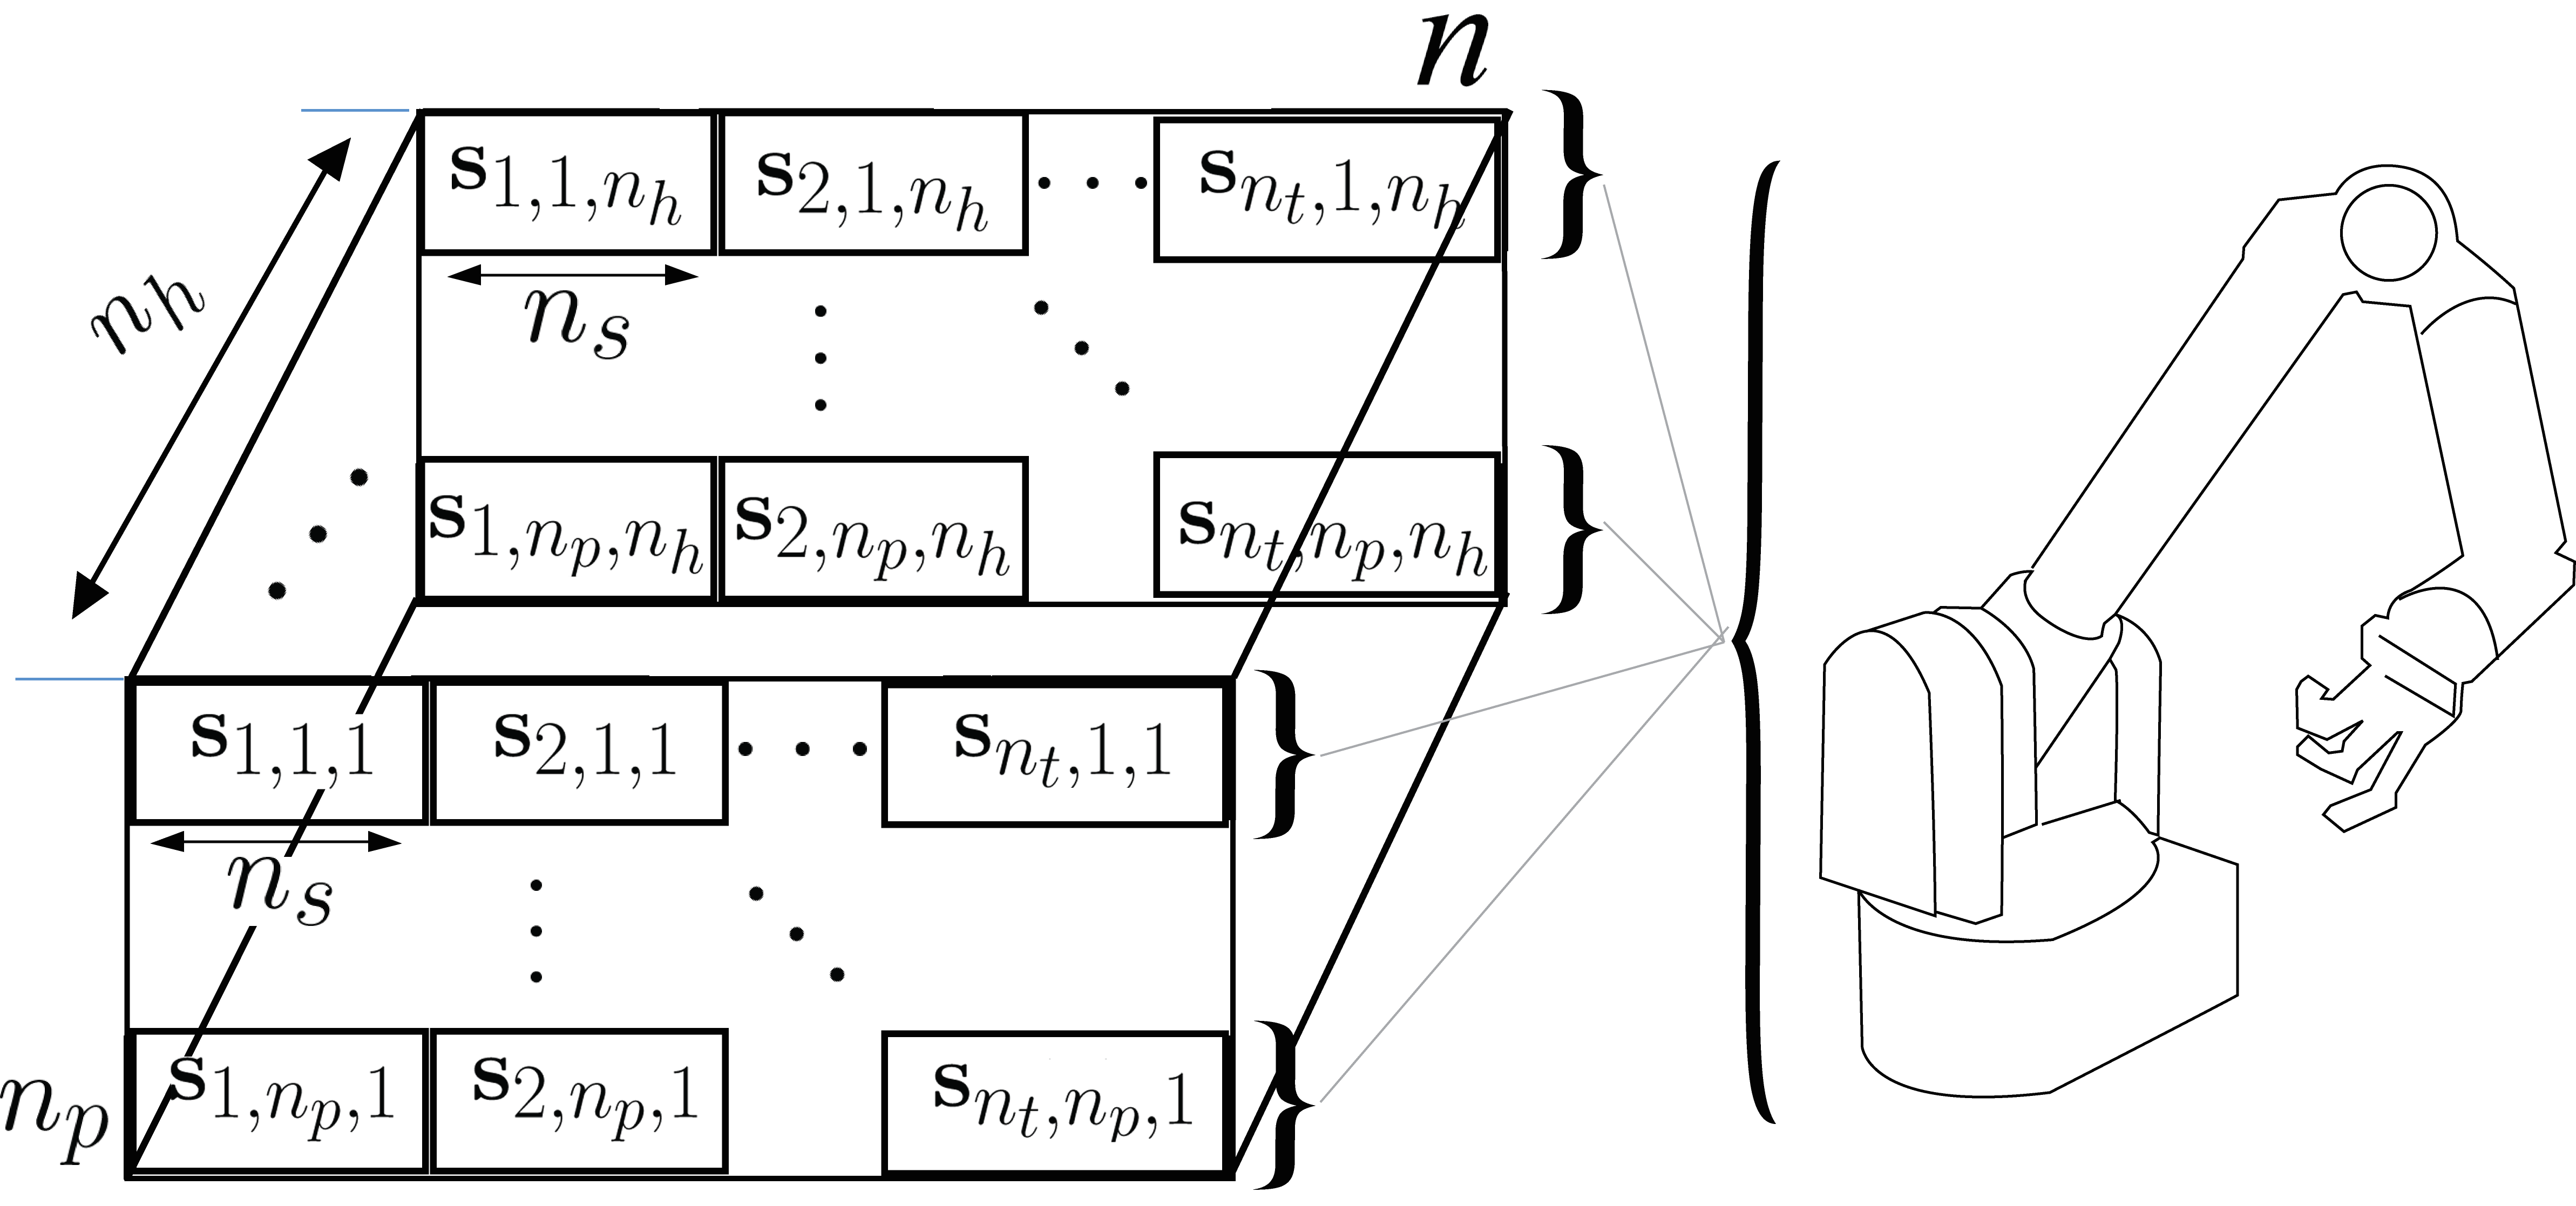
\includegraphics[width=\linewidth]{images/X_defn}  %% mass predictions
    \caption{$\mathbf{X}$}
    \label{fig:X_defn}
  \end{subfigure}
  %}
  %\fbox{
  ~~
  \begin{subfigure}[t]{0.43\linewidth}
    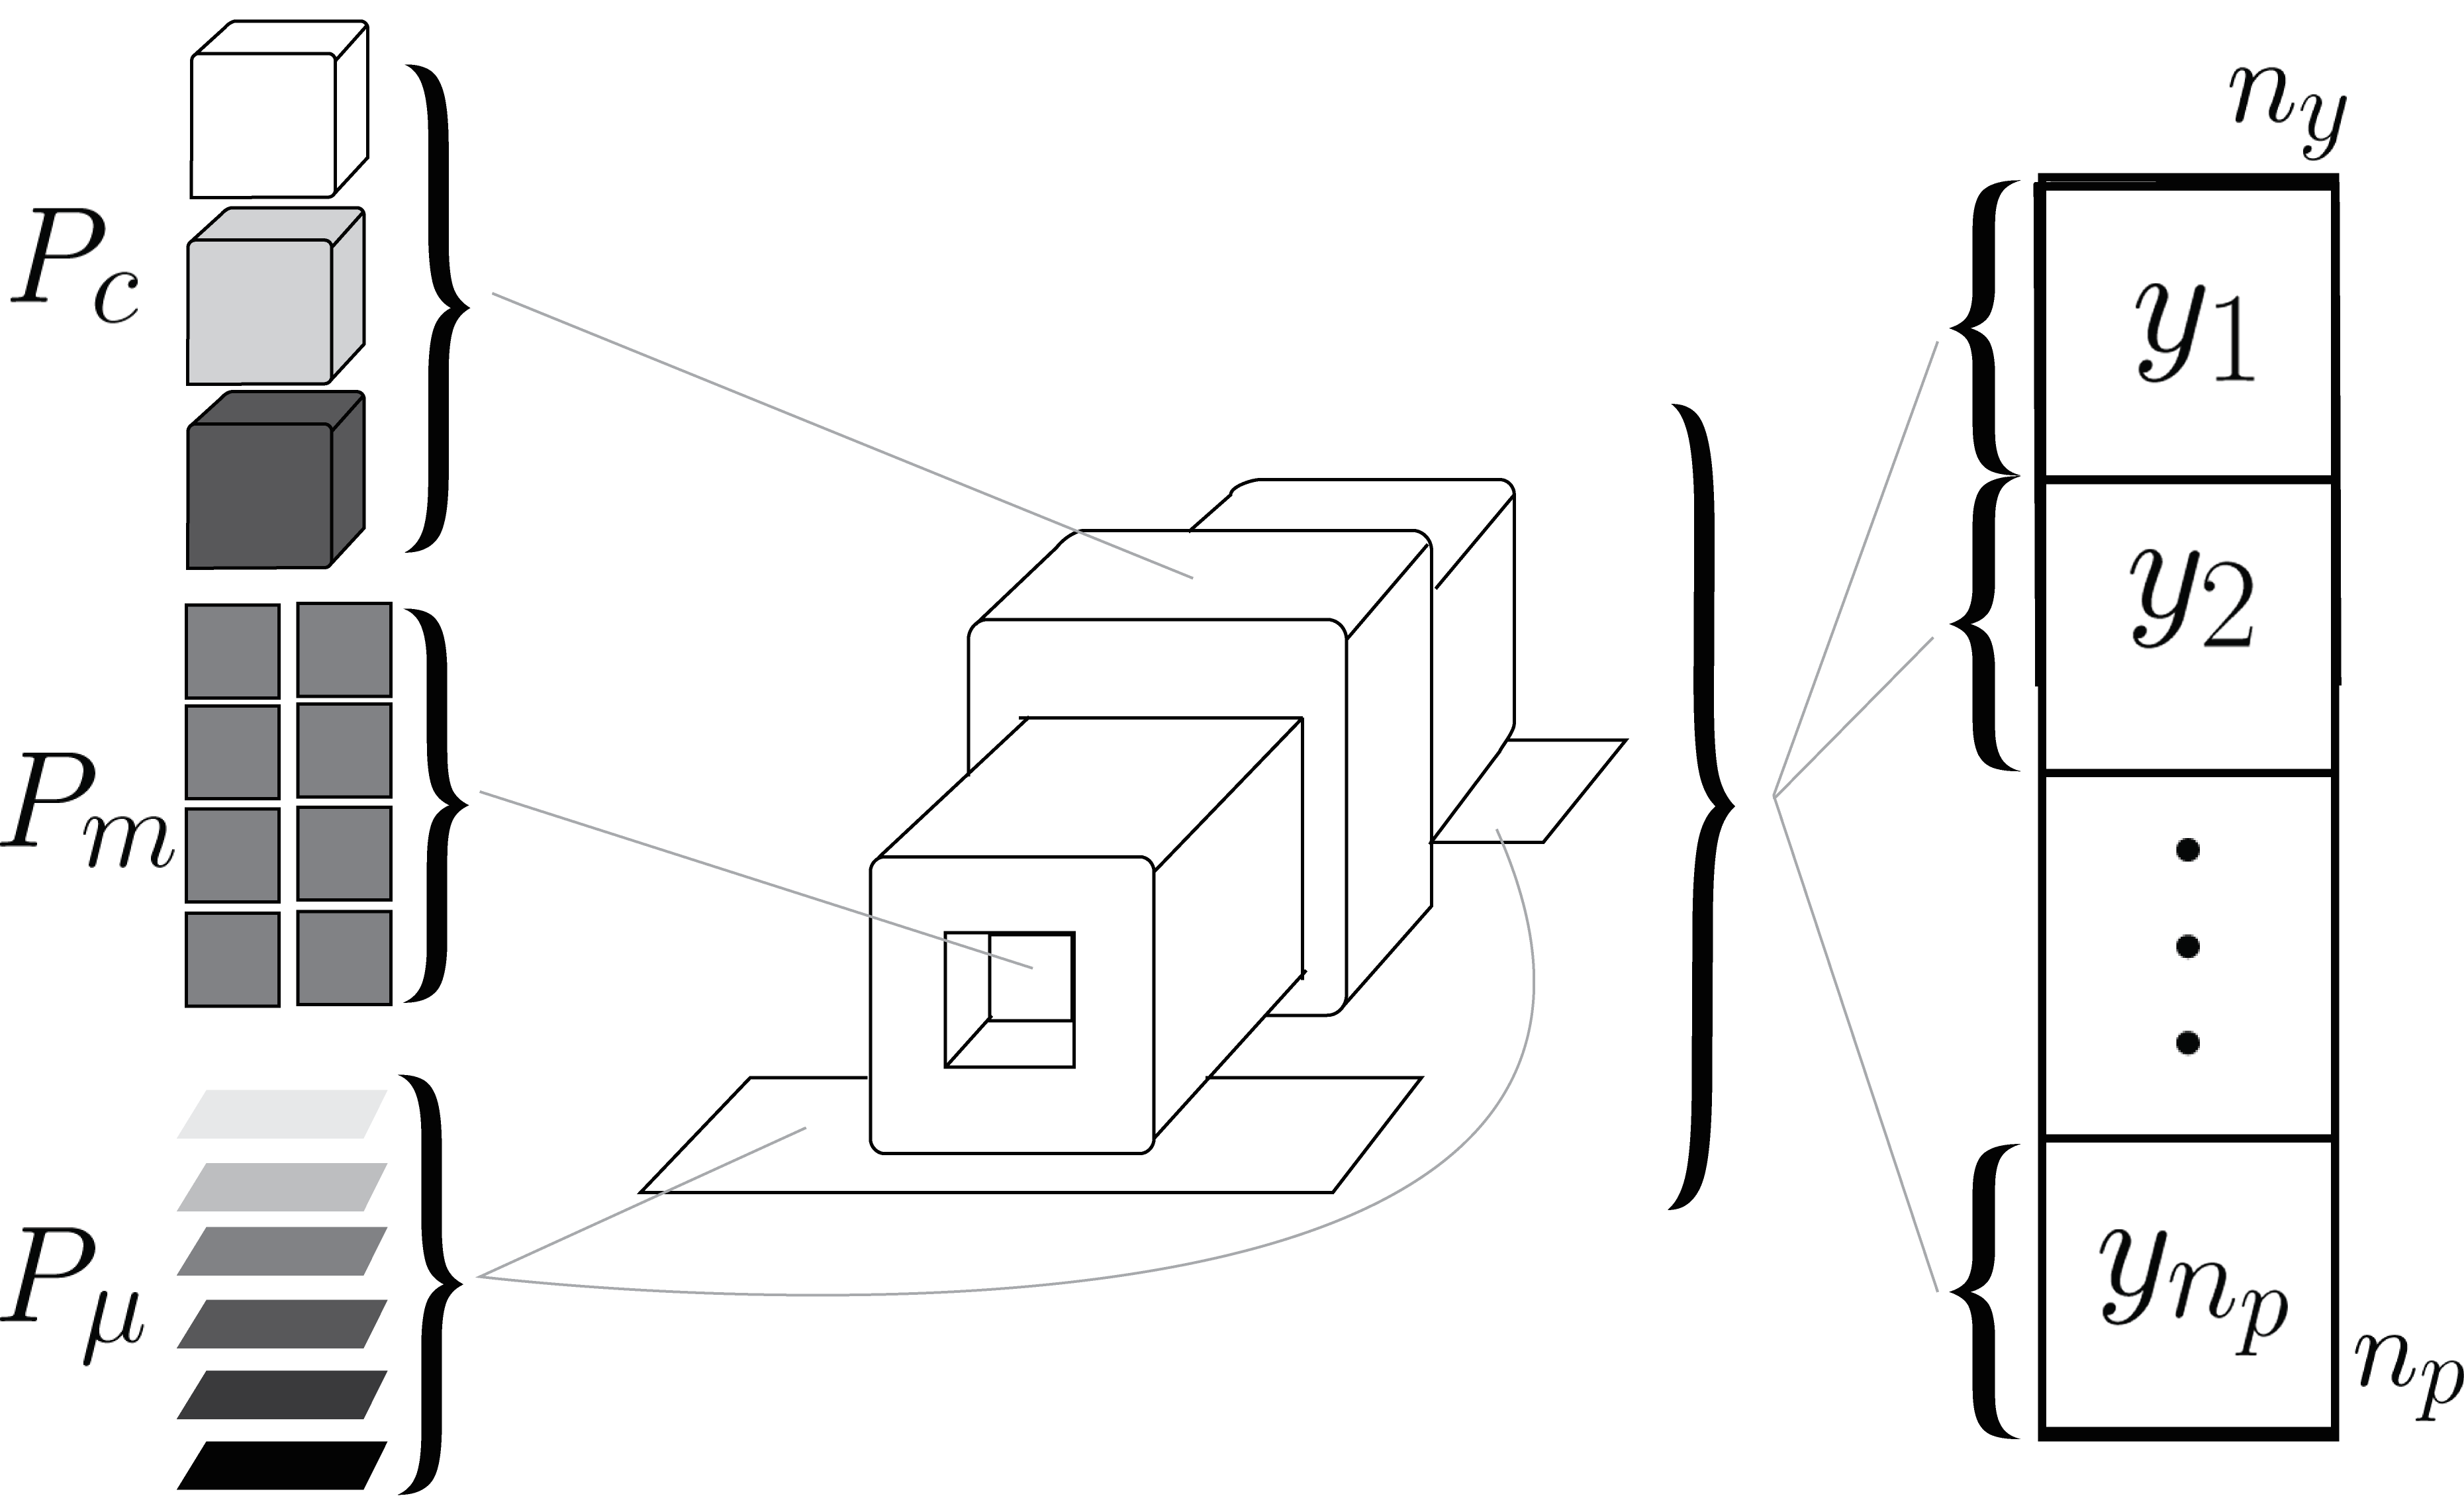
\includegraphics[width=\linewidth]{images/Y_defn}  %% mass predictions
    \caption{$\mathbf{Y}$}% provided}
    \label{fig:Y_defn}
  \end{subfigure}
  %}
  \caption{Collection of data matrix $\mathbf{D} = (\mathbf{X},\mathbf{Y})$: (a) data $\mathbf{X}$ are collected across all trials and environments; (b) environmental quantities $\mathbf{Y}$ are provided, which express each of $n_p = 144$ environments as $n_y=3$ floating point numbers.}
\end{figure}

%%% define the example motion and its purpose
The manipulation task considered is shown in Figure~\ref{fig:topple}. 
The end effector pushes down on a foam-encapsulated block, causing it to topple, then pushes the block back to its starting position against the wall.
A prescribed joint-space trajectory to achieve this manipulation task is provided by a human expert via kinesthetic teaching.
%TODO: is this really standard?
Upon replay, the robot tracks the given trajectory using standard computed-torque control.
We assume the trajectory is robust in two ways: (1) repeating the trajectory causes repeated rotations of the block, and (2) the same trajectory remains successful in toppling blocks for all mass, friction, and compliance values.
The use of a prescribed trajectory also implies an approximate correspondence between the current elapsed time within a motion and the manipulation phase.  
%While there is, by definition, no need for motion adaptation in this experimental setup, 
%The ability to predict environment properties such as mass, friction, and compliance in real-time is, we believe, an important prelude to enabling online motion adaptation.%adaptation of motions based on sensory data.

%%% define sensory data 
Each sensory sample collected at each timestep of the prescribed trajectory is defined by a sensory data stream:
\begin{equation}
\mathbf{s}\in\mathbb{R}^{n_s}:
(\rho,\dot{\rho},\tau,p,\omega,f,\alpha)
\end{equation}
  where $\rho,\dot{\rho},\tau\in\mathbb{R}^{7}$ represent respectively the angles, velocities and torque measurements of each of the seven joints of the manipulator arm, $p\in\mathbb{R}^{7}$ gives the end effector's pose measurements (3D position and 4D quaternion), $\omega \in\mathbb{R}^{6}$ is the task wrench measured via the force-torque sensor mounted to the wrist of the robot, $f \in\mathbb{R}^{4}$ are torque measurements for the joints in the robot hand, and $\alpha \in\mathbb{R}^{72}$ are tactile sensor measurements on each of the three fingers, reshaped into a single vector.

%The above definition of $s$ is valid when all sensors onboard the robot are used.
%We also perform experiments where the hand is replaced with a rigid spherical probe; thus changing both the kinematics of the arm and the sensory stream $s$ used to learn the predictive model and make subsequent predictions.

%We also build models where the robot hand is replaced by a spherical probe that is mounted to the force/torque sensor.
%For this scenario, a reduced version of $\mathbf{s}$ is defined by dropping the measurements associated with the robot hand.

A single execution of the manipulation task leads to the capture of a sensory stream, $\mathbf{x}\in\mathbb{R}^{n}$, which consists of the observations of $n_s$ sensor readings each sampled at $n_t$ points in time, and then stacked into a single vector; here, $n=n_s \times n_t$. 
%All the elements of $\mathbf{x}$ are standardized to have a zero mean and a variance of one, as measured across all trials and properties.
%This ensures that all the sensory measurements have approximately the same scale, irrespective of their origin.

%%% define environment properties 
The environment properties to be predicted from the sensory stream data are given by $\mathbf{y}\in\mathbb{R}^{3}: (m,\mu,c)$, where $m$ is the object mass, $\mu$ the coefficient of friction between the object and its support surface, and $c$ is the material compliance of the object.

%%% define training data 
In order to learn a predictive model $\mathbf{y}=f(\mathbf{x})$, training data is first gathered for $n_p$ different combinations of the environment properties, i.e., variations of mass, compliance, and friction.
For each setting, the task is repeated $n_h$ times in each environment.
The final dataset is thus defined by the following data pairs:
\begin{equation}   \mathbf{D} = (\mathbf{X},\mathbf{Y}) = \{ (\mathbf{x}_{p,h},\mathbf{y}_{p})~\lvert~p\in[1\cdots n_p],h\in[1\cdots n_h] \}. \end{equation} 


This dataset is used to learn the predictive model that we now describe.


%-------------------------------------------------------------------------------------------------------------------------------------------------
\section{Prediction Framework}

%%%%DMT%%%%
%TODO: recap on why feature selection is important (i.e. to reduce amount of data to be streamed from the robot to prediction system)
%DONE: develop an intuition for $\Gamma$ (look at Pais et al) - a figure demonstrating $\Gamma$ would help here
%TODO: form (cite?) theoretical basis for why $\Gamma$ works (Pais et al)
%TODO: propose a strategy for how this will carry over to different tasks
%TODO: can temporal information be leveraged at all (moving windows, wavelets)?
%TODO: take out classification and stick with regression throughout
%%%%%%%%%%%


%%% the predictive model

Given a new sensory stream, $\mathbf{x}_{new}$, which consists of $n_t$ samples of $\mathbf{s}$, we wish to predict the environment properties $\mathbf{y}$.
We develop a two-stage solution that consists of 
(i) selecting the most {\em relevant} input features from $\mathbf{x}$, and 
(ii) using partial least squares (PLS) to further learn a more compact latent linear subspace that is well suited to predicting environment properties.
%%%%%
%%DMT modified for simplicity 
%As we will show in the results, PLS property predictions without the initial feature selection step are not always sufficiently accurate.
%, despite its ability to exploit correlations between inputs and between inputs and outputs.
%%%%%
We now discuss these two stages in further detail.

\subsection{Feature Selection via the Task Variance Ratio}
\label{sec:feature_selection}

\begin{figure}[tb]
  \centering
  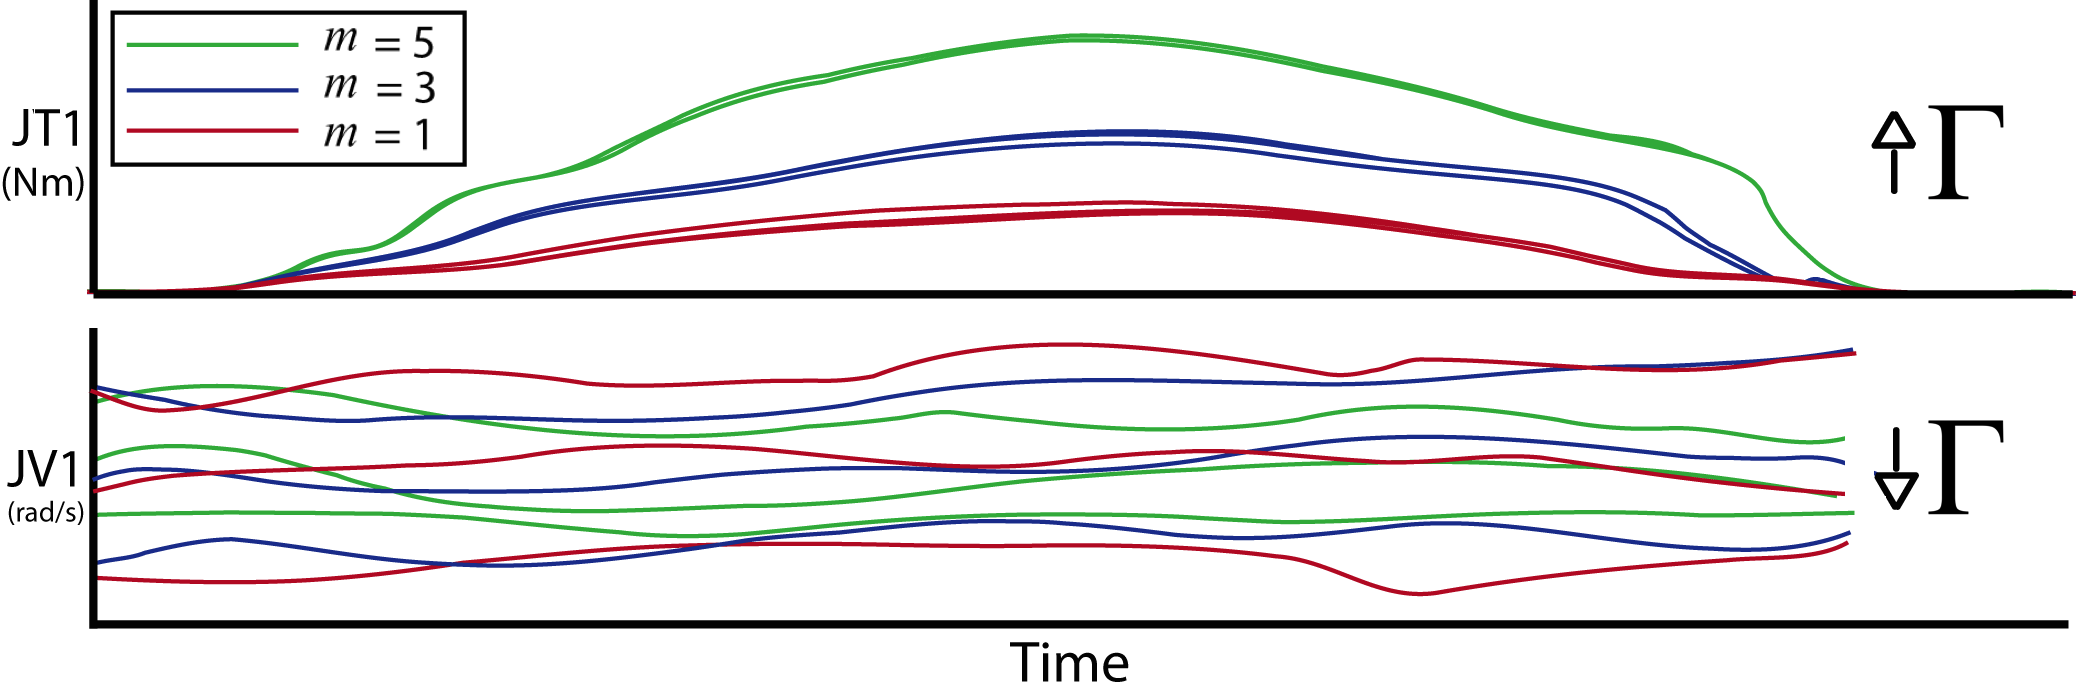
\includegraphics[width=\linewidth]{images/TVR_intuition}
  \caption{Intuition behind the task variance ratio ($\Gamma$) algorithm. We wish to select good sensors (at each time-phase) which exhibit low variance when the environment remains constant and high variance when the environment changes. Colors signify distinct environments. Multiple lines of the same color signify repeated trials within the same environment.}
  \label{fig:TVR_intuition}
\end{figure}

%\begin{figure}[t!]
%  %\fbox{
%  \begin{subfigure}[t]{0.5\linewidth}
%    \includegraphics[width=\linewidth]{images/mean_property}  %% mass predictions
%    \caption{$\mathbf{x}_{p}$}
%    \label{fig:mean_property}
%  \end{subfigure}
%  %}
%  %\fbox{
%  \begin{subfigure}[t]{0.46\linewidth}
%    \includegraphics[width=\linewidth]{images/mean_trial}  %% mass predictions
%    \caption{$\mathbf{x}_{h}$}
%    \label{fig:mean_trial}
%  \end{subfigure}
%  %}
%  %\fbox{
%  \\
%  \begin{subfigure}[t]{0.46\linewidth}
%    \includegraphics[width=\linewidth]{images/var_property}  %% mass predictions
%    \caption{$\sigma^2_{enviro}$}% provided}
%    \label{fig:var_property}
%  \end{subfigure}
%  %}
%  \begin{subfigure}[t]{0.5\linewidth}
%    \includegraphics[width=\linewidth]{images/var_trial}  %% mass predictions
%    \caption{$\sigma^2_{trial}$}% provided}
%    \label{fig:var_trial}
%  \end{subfigure}
%  \caption{Visualization of $\Gamma$ calculation. First, mean sensor readings across property sets (a) and trials (b) are calculated from data $\mathbf{X}$. Next, the variance of these mean sensor readings are calculated (c,d). Finally $\Gamma$ is defined as the ratio of the two variance vectors.}
%%a) mean sensor readings within each property set and across all trials; b) mean sensor readings within each trial and across all property sets; c) variance of mean sensor readings across property sets; d) variance of mean sensor readings across trials.}
%  \label{fig:TVR_calculation}
%\end{figure}

%%%%%
%%DMT added:
%As mentioned previously, due to limited resources, systems embedded on robotic hardware typically cannot process large amounts of input data in real-time.
%%%%%%
%To cope with the high dimensional nature of the sensory stream data, we first describe a selection mechanism that is well suited to identifying specific sensors and sample times that are likely to be informative for the prediction problem.
%\begin{equation}   \mathbf{D} = (\mathbf{X},\mathbf{Y}) = \{ (\mathbf{x}_{p,h},\mathbf{y}_{p})~\lvert~p\in[1\cdots n_p],h\in[1\cdots n_h] \}. \end{equation} 
We define the {\em Task Variance Ratio ($\Gamma$)} vector as
%   \begin{equation}  \Gamma = {\frac{\sigma^2_{enviro}}{\sigma^2_{trial}} | } ,\end{equation}
\begin{equation} \Gamma = \{\Gamma^i=\frac{\mathit{Var}_i^{enviro}}{\mathit{Var}_i^{trial}}~\lvert~i\in[1\cdots n] \} \end{equation}
where $\mathit{Var}_i^{trial}$ models the variance of a given element of $\mathbf{X}$ across all trials, 
and $\mathit{Var}_i^{enviro}$ models the variance of the same element across all environments. 
Specifically, 
   %\begin{equation}\sigma^2_{trial} = \frac{\sum{(\mathbf{x}_{h}-\bar{\mathbf{x}_{h}})^2}}{n_h-1},\end{equation}
  \begin{equation}\mathit{Var}_i^{trial}=\frac{\sum_{h=1}^{n_h}({\mathit{x}_{i,h})^2}-\frac{(\sum_{h=1}^{n_h}{\mathit{x}_{i,h}})^2}{n_h}}{n_h-1}\end{equation}
%i.e., the variance of the given element as computed using all available measurements (all properties $p$ and trials $h$) in $\mathbf{D}$, 
and 
   %\begin{equation}\sigma^2_{enviro} = \frac{\sum{(\mathbf{x}_{p}-\bar{\mathbf{x}_{p}})^2}}{n_p-1},\end{equation}
  \begin{equation}\mathit{Var}_i^{enviro} = \frac{\sum_{p=1}^{n_p}{(\mathit{x}_{i,p})^2}-\frac{(\sum_{p=1}^{n_p}{\mathit{x}_{i,p}})^2}{n_p}}{n_p-1}\end{equation}
%i.e., the mean of the $n_p$ variances that can be computed when measurements are grouped according to environment properties.
for all $i \in [1\cdots n]$.

A large value of $\Gamma_i$ indicates a good feature, as it implies that variation occurs as changes to the environment take effect, while observable noise between repeated trials in the same environment is relatively small.

%\begin{equation}\mathbf{X}_{h} = \frac{1}{n_p}\sum_{p=1}^{n_p}{\mathbf{x}_{p,h}}~\lvert~ h\in[1\cdots n_h]\end{equation} and

The feature selection is then implemented using a simple threshold function to produce a reduced input matrix $\mathbf{X}^*$:
   \begin{equation} \mathbf{X}^* = \mathbf{X}_p \cdot diag(\Gamma > \Gamma_{\min}),\end{equation} 
where
\begin{equation}\mathbf{X}_{p} = \frac{1}{n_h}\sum_{h=1}^{n_h}{\mathbf{x}_{p,h}}~\lvert~ p\in[1\cdots n_p],\end{equation} 
$diag(v)$ produces a square matrix with the elements of $v$ across the diagonal, and $\Gamma_{min}$ is chosen such that the desired number of elements of $\Gamma$ are selected.
%where $i\in[1\cdots n_sn_t]$, $p\in[1\cdots n_p]$, and $h\in[1\cdots n_h]$.
%\begin{equation} 
%\mathbf{x}_i^*= 
%\left\{
%\begin{matrix*}[l]
%1\; if\;  \Gamma_i >\Gamma_{min}
%\\ 
%0\;\; otherwise
%\end{matrix*}
%\right.
%\end{equation}
The resulting reduced dataset is given by
\begin{equation}   \mathbf{D}^* = (\mathbf{X}^*,\mathbf{\mathbf{Y}}) = \{ (\mathbf{x^*}_{p},\mathbf{y}_{p})~\lvert~ p\in[1\cdots n_p] \}. \end{equation} 

In this way, we identify features in $\mathbf{X}$ that exhibit small variation across repeated trials when the environment is kept constant and exhibit large variations as the environment changes (see Figure~\ref{fig:TVR_intuition}), which we approximate as the degree of relevance of the sensor reading to predicting environment properties.

\subsection{Property prediction with Partial Least Squares}
\label{sec:PLS}

% is an effective prediction method in high-dimensional settings such as the one encountered here.

The PLS algorithm provides us with an estimated weighting matrix $\mathbf{\beta} \in \mathbb{R}^{c\times n_y}$, where $c$ is a parameter denoting the number components to factor.

$\beta$ is calculated iteratively according to the following algorithm:
first, define 
\begin{equation}
\begin{aligned}
A_0& = \mathbf{X^{*T}}\mathbf{Y}, \\
M_0& = \mathbf{X^{*T}}\mathbf{X^*},&& \text{and} \\
C_0& = I,\\
\end{aligned}
\end{equation}
then iterate
\begin{equation}
\begin{aligned}
q_j& = eigv1(A^T_{j-1}A_{j-1}) && \text{$q_j \rightarrow$ dominant eigenvector} \\
w_j& = A_{j-1}q_j \\%&& \text{blah}\\
c_j& = w^T_jM_{j-1}w_j \\%&& \text{blah}\\
w_j& = \frac{w_j}{\sqrt{c_j}} && \text{store into column j of W}\\
r_j& =M_{j-1}w_j && \text{store into column j of R}\\
q_j& =A^T_{j-1}w_j && \text{store into column j of Q}\\
v_j& =\eta C_jp_j && \text{$\eta \rightarrow$ normalizing constant}\\
C_j& =C_{j-1}-v_jv_j^T \\%&& \text{blah}\\
A_j& =C_jA_{j-1} \\%&& \text{blah} 
\end{aligned}
\end{equation}
for all $j \in [1 \cdots c]$.
With $R$, $Q$ and $W$ assembled, we now compute: 

\begin{equation}
%\begin{aligned}
\beta = WQ^T
%\end{aligned}
\end{equation}

  %\begin{equation} \beta = PLS(\mathbf{D}^*). \end{equation}
Finally, we use $\beta$ at runtime to predict environment properties:
  \begin{equation} \mathbf{\hat{y}} = \mathbf{\beta} \cdot \mathbf{x^*_{new}} \end{equation}

Data from multiple haptic sensors are likely to be highly correlated, e.g. Cartesian force experienced by the hand and tactile pressure readings at the fingertips.
In addition, there is likely to be significant correlation between sensor readings over time.
Lastly, there are correlations between the input dimensions and output dimensions.
The existance of these correlations are ideal in the application of the PLS  regression method \cite{Tobias1995}.
%--------------------------------------------------------------------------------------------------------------

\chapter{Control Software}
\label{chap4}

In this chapter, we provide an overview of the software deployed to control the motion of the robot and collect sensor readings in support of experiments.

%\section{Usage}
%\section{Maintenance}

\section{System Overview}
To support experiments, a sensor processing and robot control framework was written in C++ leveraging the libbarrett API provided by Barrett Technology Inc (Section~\ref{sec:libbarrett}). 
Our framework was developed exclusively on the internal PC of the WAM robot \cite{townsend1993mechanical}, the details of which are presented in Table~\ref{tbl:wam_specs}.
%For more details on the hardware specifications, please see Appendix~\ref{apx_B}.

\begin{table}[h]
\centering
\begin{tabular}{|l|l|}
\hline
Motherboard        & Aaeon PFM-540I                    \\
Processor          & 500 MHz AMD LX-800 x86-compatible \\
Memory             & 256 MB 200-pin DDR-333 SODIMM     \\
Linux distribution & Ubuntu 9.10                       \\
Linux kernel       & 2.6.31.4                          \\
Realtime           & Xenomai 2.5                       \\
Ethernet           & 10/100 Base-T                     \\
CANbus             & Peak PCAN-PC/104, 2 ports         \\ \hline
\end{tabular}
\caption{Specifications of the WAM Internal PC/104 \cite{wam_specs} used for framework development and robot control in support of experiments.}
\label{tbl:wam_specs}
\end{table}

\section{Libbarrett API}
\label{sec:libbarrett}

The API used to communicate with the robot is called libbarrett: a C++ library from Barrett Technology Inc. \cite{libbarrett}.
Our framework was tested using version 1.1.0 of the API.
The libbarrett API provides abstract control of the WAM and BarrettHand and allows them to be controlled in tandem.
Sample programs that perform simple control and sensor monitoring routines are provided, upon which our controller in the current study is based.

Libbarrett provides three high-level constructs to interface with the robot: (1) the WAM object (2) the Hand object and (3) the ProductManager object.
The WAM and Hand objects provide high-level control of the WAM and attached BarrettHand respectively.
The ProductManager provides access to the WAM's optional components, such as attached tools (e.g.  BarrettHand) and Force/Torque sensor.
The control software communicates with the Hand and WAM through high-level function calls to their respective libbarrett objects using a variety of pre-defined data structures. 
These datastructures are presented in Table~\ref{tbl:data_types}.
%Data types for interfacing with the WAM and BarrettHand are presented in Table~\ref{tbl:data_types}.

\begin{table}[h]
\centering
\begin{tabular}{| c | c | c |}
    \hline
    Name & Type & Unit \\
    \hline 
    Cartesian Position & cp\_type & Meters\\
    Joint Position & jp\_type & Radians\\
    Joint Velocity & jv\_type & Radians/s\\
    Joint Torque & jt\_type & Radians/s \\
    \hline 
\end{tabular}
\caption{Libbarrett data-types when communicating with the robot. The jp\_type for the WAM is a seven-dimensional vector whereas for the BarrettHand, it is a four-dimensional vector -- one entry for each finger and one for the spread.}
\label{tbl:data_types}
\end{table}


\section{WAM Control}

\paragraph{Cartesian-space}
Control in Cartesian space is a convenient way to prototype motions and is sufficiently repeatable for tasks which require low accuracy.
Accuracy of the Cartesian positioning of the WAM is advertised at two millimeters.
In practise, however, this accuracy depends largely on the joint-angle configuration of the WAM at the beginning of the Cartesian-space move.
In our experiments, position error could easily accumulate to reach as high as one centimeter, depending on the joint-angle position of the robot at the beginning of the Cartesian-space move.
These high errors may be due to imperfect inverse-kinematics currently available through the libbarrett API.
%Hand-tuned motions are more easily accomplished in Cartesian space when a specific motion within is desired and is effective only if the level of accuracy required is relatively low (0.5~1 cm).
Cartesian trajectories were not sufficiently repeatable in our experiments since we required a precise and highly repeatable motion (accurate to within 1 mm) to perform our task across various environments.
Moreover, the workspace accessible by rotating the wrist is limited by the angular configuration of its attaching joint. 
This means that certain wrist orientations are not repeatable if the inverse-kinematics solution provides differing joint-space positioning around the wrist.
These drawbacks prevent us from commanding the robot in Cartesian-space in our experiments.
%which is a limitation we have encountered in our experiments.
%Since motion of the robot is desired within a specific area of the workspace, the simplest and most straightforward 

\paragraph{Joint-space}
For accurate and repeatable sets of motions, the robot should be controlled directly in joint-space.
%This is problematic when developing motions by hand since specific Cartesian-space trajectories are extremely difficult to match via specific hand-tuned joint-angle trajectories.
The only issue with joint-space control is that the robot performs its task in Cartesian-space. 
Joint-angle trajectories that accomplish specific Cartesian-space tasks are difficult if not impossible to define manually.
This necessitates kinesthetic teaching where the robot is trained to perform its task in Cartesian space by a human expert manually moving the robot tool to perform a task, while corresponding joint-space trajectories are recorded by the robot.

\paragraph{Kinesthetic Teach-and-Play}
The libbarrett API comes equipped with kinesthetic teaching functionality via the teach-and-play module.
Teach-and-play records position information at the rate of 500Hz while a user physically moves the robot through the desired motions.
The robot can record its trajectory in either Cartesian-space or joint-space.
Again, due to imperfect inverse-kinematics, if a highly repeatable motion is required it is advisable to record trajectories in joint-space.
It becomes possible to execute highly repeatable Cartesian-space trajectories if the relative displacement from a known starting joint-angle position is small (i.e. a workspace of approximately $10cm^3$ around a starting joint-angle position).

\section{BarrettHand Control}

In this section, we introduce the details on control of the BH8-280 BarrettHand through the libbarrett API, as used in our experiments.

\paragraph{Velocity Move}
The simplest form of control of each finger of the Hand is to specify a direction and rate of travel of each of the joints in the Hand.
The joints will halt gracefully if they reach their limits or become obstructed before they reach these limits.

\paragraph{Trapezoidal Position Move}
If the Hand must be configured precisely (for e.g a pre-grasp posture), the user can specify desired joint-angles of each finger and spread.
The spread of the Hand refers to the single degree of freedom rotation of the first and third fingers about the palm.
Upon sending position commands the hand, the proximal finger joint angles or the angle of spread move toward the goal position via a trapezoidal velocity profile.
As with velocity control, the fingers will halt gracefully if the movement of the hand becomes obstructed.

\paragraph{High Control-rate Position Move}
High control-rate position moves provide an advanced alternative to simple trapezoidal moves.
Joint-angles can be specified to reach a desired pose, however each of the joints travel at maximum velocity until they reach the desired pose or become obstructed.
Care must be taken when sending these commands, as obstructions do not result in graceful halts and instead could cause damage to objects or the Hand itself.
It is necessary to ensure a clear path for each of the fingers and spread of the Hand before sending these commands.

\section{Realtime Systems}
\label{sec:realtime_eg}
Control of the robot in realtime must be done through the libbarrett realtime systems API.
Realtime control allows for complex and closed-loop motions since the output of each realtime system depends upon its inputs at each step of the realtime control loop at the rate of 500Hz.
Program~\ref{pgm:rtsys} provides an example program which defines such a realtime system in the C++ programming language.

\begin{landscape}
\begin{Program}[width=0.5\pagewidth]
\center
\begin{verbatim}
class WamSystem : public System {
public:     Input<jp_type> input;       // Obtain current joint-angles as input
public:     Output<jp_type> output;     // Provide updated joint-angles as output
protected:  Value* outputValue;         // Value that output reads
protected:  jp_type jp_offsets;         // Modifications to realtime motion feed
public:
    WamSystem(const string& sysName):   // All systems must define a name
        System(sysName), input(this), output(this, &outputValue){ 
            init_vec(&jp_offsets, 0);   // Initialize all offsets to 0
        }
    ~WamSystem(){ mandatoryCleanUp(); } // Mandatory destructor 
protected:
    jp_type jp_out;                     // Declare local copy of output data
    virtual void operate() {
        const jp_type& jp_in = input.getValue();    // Pull data from the input
        jp_offsets[5] += 0.001;         // Increase 6th joint-angle of WAM slightly
        jp_out = jp_in + jp_offsets;    // Modify wam joints by relative offsets
        outputValue->setData(&jp_out);  // Push data to subsequent system
    }
};
\end{verbatim}
  \caption{Example libbarrett realtime system written in C++ that controls the 6th joint of the WAM to increase indefinitely. Namespace references removed for brevity.}
  \label{pgm:rtsys}
\end{Program}
\end{landscape}

%%%%%%%%%%%%%%%%%%%%%%%%%%%


\chapter{Experiments and Results}
\label{chap5}

In this chapter, we describe the experimental setup, provide details on the experimental procedure, and finally present and discuss environment property prediction results obtained by using the prediction framework.


\section{Setup}

\subsection{Actuation and Sensing}
\label{sec:actuation_and_sensing}

Experiments are conducted using a 7 DOF Barrett WAM robot arm with attached 4 DOF Barrett BH-280 Hand, built by Barrett Technology (MA, USA).
A 6-axis force-torque sensor is mounted to the wrist of the arm.
The robot hand is equipped with tactile arrays on the fingers and palm.
Joint torque sensors are embedded in each of the 3 fingers.
Position control of the arm occurs at 500Hz and all sensors are sampled at 125~Hz, which is reduced to 2.5~Hz during preprocessing~(see section~\ref{sec:preprocess}).

\subsection{Kinesthetic Teach and Play}
\label{sec:kinesthetic_teach_and_play}

Example trajectories are demonstrated to the robot via a kinesthetic teach-and-play interface.
The system records pose estimates of the arm at the rate of 500~Hz and the result is saved for future playback.

\subsection{Software Architecture}
\label{sec:software_architecture}

Our real-time control framework runs on top of the {\em libbarrett} real-time systems library \cite{libbarrett}, and is used during demonstration and autonomous execution.
We also use it to record and play back data streams that are time-synchronized with the motion.
See Chapter~\ref{chap4} for further details.

\subsection{Experimental Testbed}
\label{sec:testbed}

The block used for the experiment is a rectangular prism made of medium-density polyethylene foam, with length 48.5~cm, width 10.5~cm and height 10.5~cm.
Two parallel walls of length 28.5~cm and width 6.5~cm are used to prevent the block from sliding sideways out of the workspace.
The distance between the walls is 49~cm.
As shown in Figure~\ref{fig:topple}, a wall is used to limit the final sliding motion and leave the block in its original location, ready to be toppled again.
The walls are lined with paper to decrease the coefficient of friction between the block and the walls for smoother operation.


In our experiments, different environments are defined by the Cartesian product of three sets of environment property values for $P$ = \{$P_{m}$, $P_{\mu}$, $P_{c}$\}, yielding a total of $8 \times 6 \times 3 = 144$ different environments.
These values are shown in Table~\ref{table:property_set}.

\begin{table}[h]
\centering
\begin{tabular}{l|l}
$P_m$ (g)   & \begin{tabular}[c]{@{}l@{}}425, 650, 875, 1100,\\ 1325, 1550, 1775, 2000\end{tabular} \\ \hline
$P_\mu$      & \begin{tabular}[c]{@{}l@{}}0.441, 0.505, 0.616,\\ 0.768, 0.911, 1.136 \end{tabular}            \\ \hline
$P_c$ (mm/N) & 0.294, 2.484, 0.978
\end{tabular}
\caption{Mass, coefficient of Coulomb static friction and compliance property sets, as measured for a variety of blocks and surfaces.}
\label{table:property_set}
\end{table}

\subsection{The Block Topple-Slide Task}

Toppling, as defined in \cite{Lynch1999}, consists of two high-level phases: rolling and settling.
In the rolling phase, the robot pushes the block up onto a toppling edge, which is perpendicular to the robot's movement, until the center of mass of the block is directly above the edge.
During the settling phase, the block falls under gravity and lands on a new face before coming to rest.

As it is difficult to ensure the block's center of mass is above the edge following the rolling phase, the prescribed motion is developed so as to have the robot maintain contact with the block throughout the settling phase, to the extent that this is possible.

Once the block has settled, the robot then proceeds to slide the block across the surface of the table until the block has come to a stop back at its initial pose.
Figure~\ref{fig:topple} depicts the topple-slide task with a sequence of images.

\section{Procedure}

%%%%DMT%%%%
%TODO: cut down the detail! (maybe a simple graphic would suffice)
%%%%DMT%%%%

\subsection{Learn the Task Trajectory}

A human expert demonstrates the topple-slide trajectory (Figure~\ref{fig:topple}) via kinesthetic teaching.
The robot is fixed to the table so as to not introduce additional variance in the recorded data due to base motion.
The demonstrating user performs the task in about 6~s.  
The motion is then manually tuned so that the reference trajectory succeeds for the topple-slide task for a variety of combinations of block mass, coefficient of friction, and compliance (see section~\ref{sec:actuation_and_sensing}).

\subsection{Record Sensory Dataset $\mathbf{D}$}
\label{sec:preprocess}

The prescribed motion is repeated over a series of trials $h \in [1\cdots n_h]$ for each property set $p \in P$, yielding the complete raw sensory data set $D$. 
We use $n_h=20$ repeated trials.
Before training our model, we pre-process the data as follows.
The sensory data is resampled to 5~Hz after applying a 200~ms mean box filter. 

We whiten each data set to support meaningful comparisons between sensors -- by shifting data collected from each sensor to have zero mean and a variance of one -- across all trials $h \in [1 \cdots n_h]$ and property sets $p \in P$.  
In our experiments we use $n_s=110$ sensors across $n_t=18$ time samples.
This yields a complete input vector of size $n = 1980$ for each manipulation trial.

\subsection{Feature Selection}

Following the equations in section \ref{sec:feature_selection}, we compute the $\Gamma$ for each element in $\mathbf{x}$.
We select $\Gamma_{\min}$ so as to select $0.1 \times n$ features.% in order to achieve an appropriate balance between bias and variance.
%In practice, we keep only 5\% of the original sensory features while increasing the prediction accuracy as compared to the default of using the unreduced set.

\subsection{Partial Least Squares Modeling}
Following PLS, we obtain the $\mathbf{\beta}$ coefficients.
We can make the representation more compact by further choosing only the $\mathbf{\beta}$ coefficients of largest magnitude.
In practice, we are able to make a further reduction of around 40\% without any significant impact on the prediction accuracy, as shown in Figure~\ref{fig:beta_reduc_comp}.
The first row uses all features and no PLS reduction.  
The second row uses a reduced set of 5\% selected features without PLS reduction. 
The third row uses 5\% selected features, followed by 40\% PLS reduction. 
%Following feature extraction step, the first and last time-phase of the motion are deemed irrelevant to the estimation task.

%FIGURE 
\begin{figure}[]
	\centering
	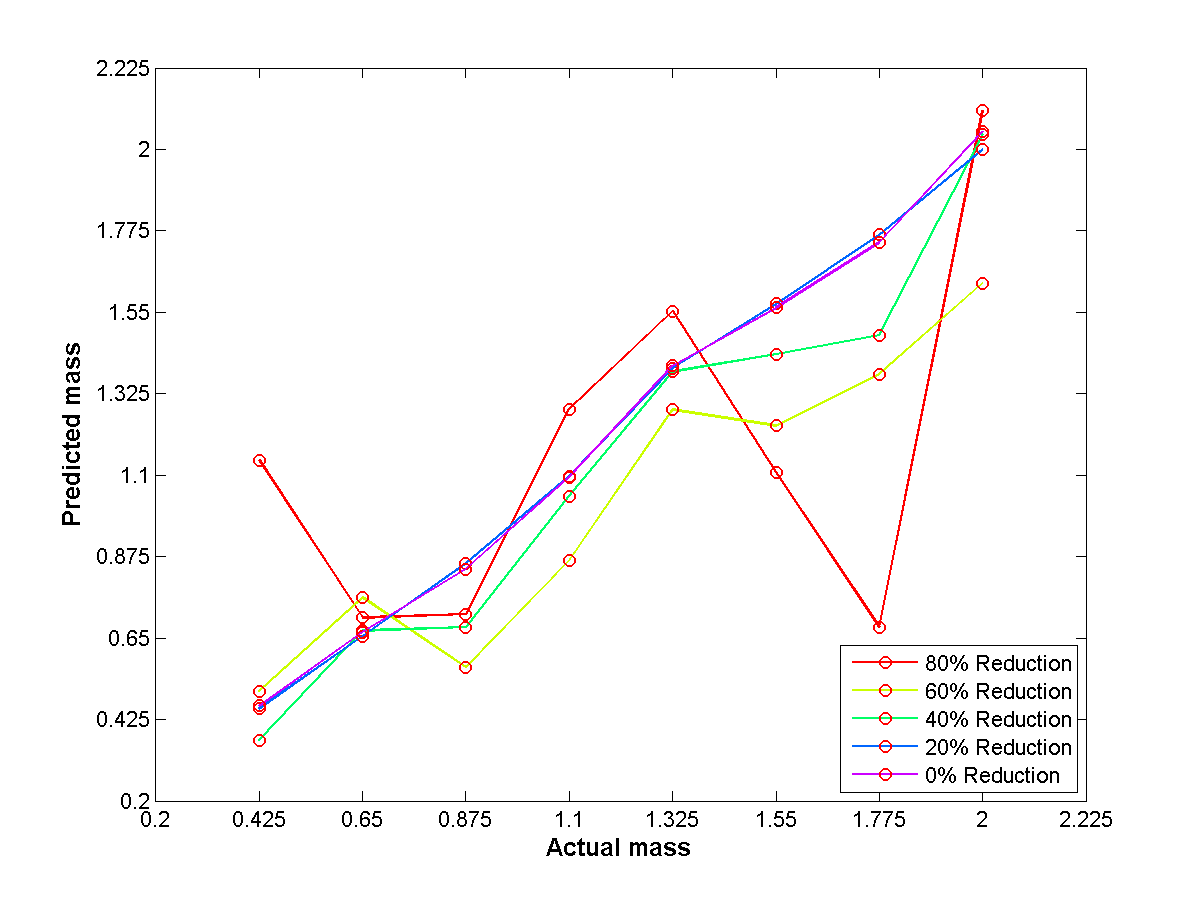
\includegraphics[width=\linewidth]{images/beta_reduc_comp}
	\caption{Effect of varying degrees of PLS dimensionality reduction on mass estimation performance. A 20\% reduction is achievable with trivial loss in estimation quality.}
	\label{fig:beta_reduc_comp}
\end{figure}
%ENDFIGURE

\subsection{Online Prediction}

%Once the model has been established using the above steps, it can be run in real-time on-board the robot as it collects novel sensory stream data during the block topple-slide task.
%%%%%
%%DMT removed:
%%As one would expect, the prediction of environment properties is most accurate once the robot has accumulated sensor readings throughout the entire motion.
%%However, we are also able to make predictions in an on-demand fashion, without having to wait until the entire motion has completed.
%%%%%
We start by parsing the entire motion into a series of key time-phases, $t^*$.
We define each $t^* \in T$ as a time-phase wherein at least $K$ sensors have received a $\Gamma$ larger than a certain value.
%This ensures that we make predictions only once it actually plausible to do so.
In practice, we choose a minimum $\Gamma$ so that $K=0.1 \times n_s$.
By training separate models in this fashion, we are able to make predictions as soon as the robot enters any phase of the motion involving selected features.
Figures~\ref{fig:online}~and~\ref{fig:online_mfc_vid} demonstrate the prediction performance on-board the robot as it executes the task.

%FIGURE 
\begin{figure}[]
	\centering
	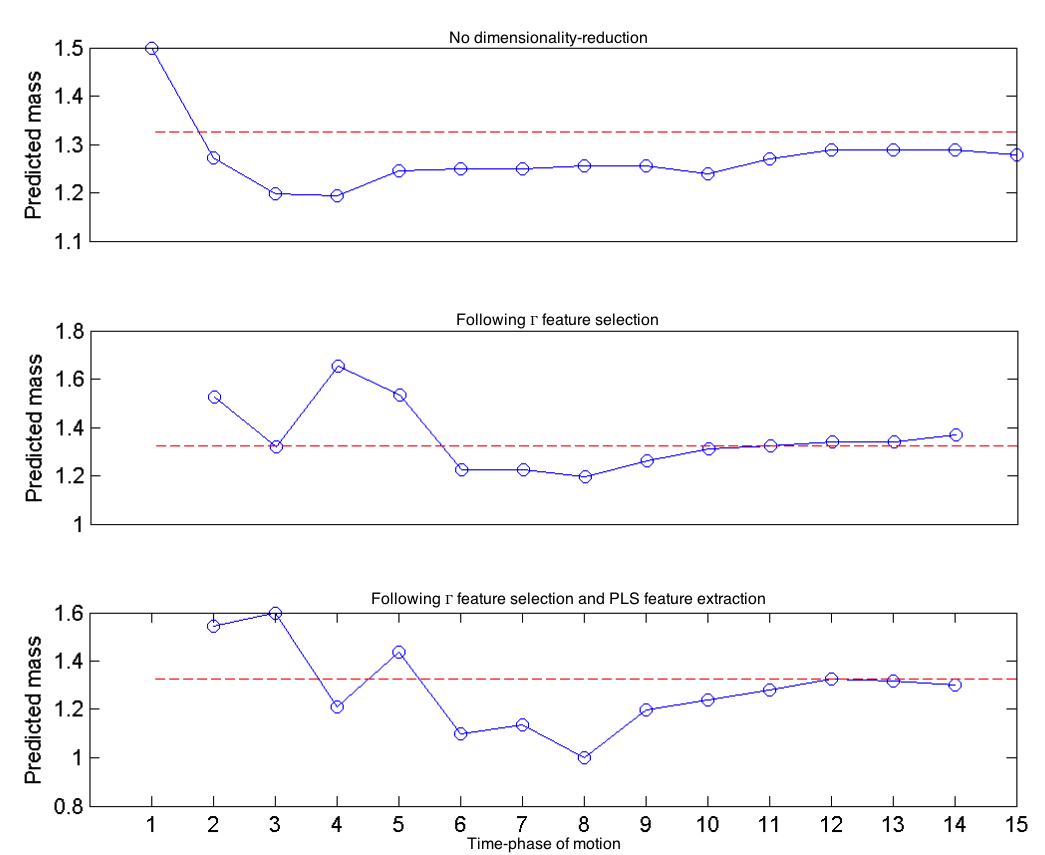
\includegraphics[width=\linewidth]{images/online_m}
	\caption{Online estimation of the mass from sensory data using varying degrees of dimensionality reduction. The estimated mass of the block are shown at various blue points throughout the motion. The dotted red horizontal line denotes the actual mass of the block. }
	\label{fig:online}
\end{figure}
%ENDFIGURE

%FIGURE 
\begin{figure}[]
	\centering
	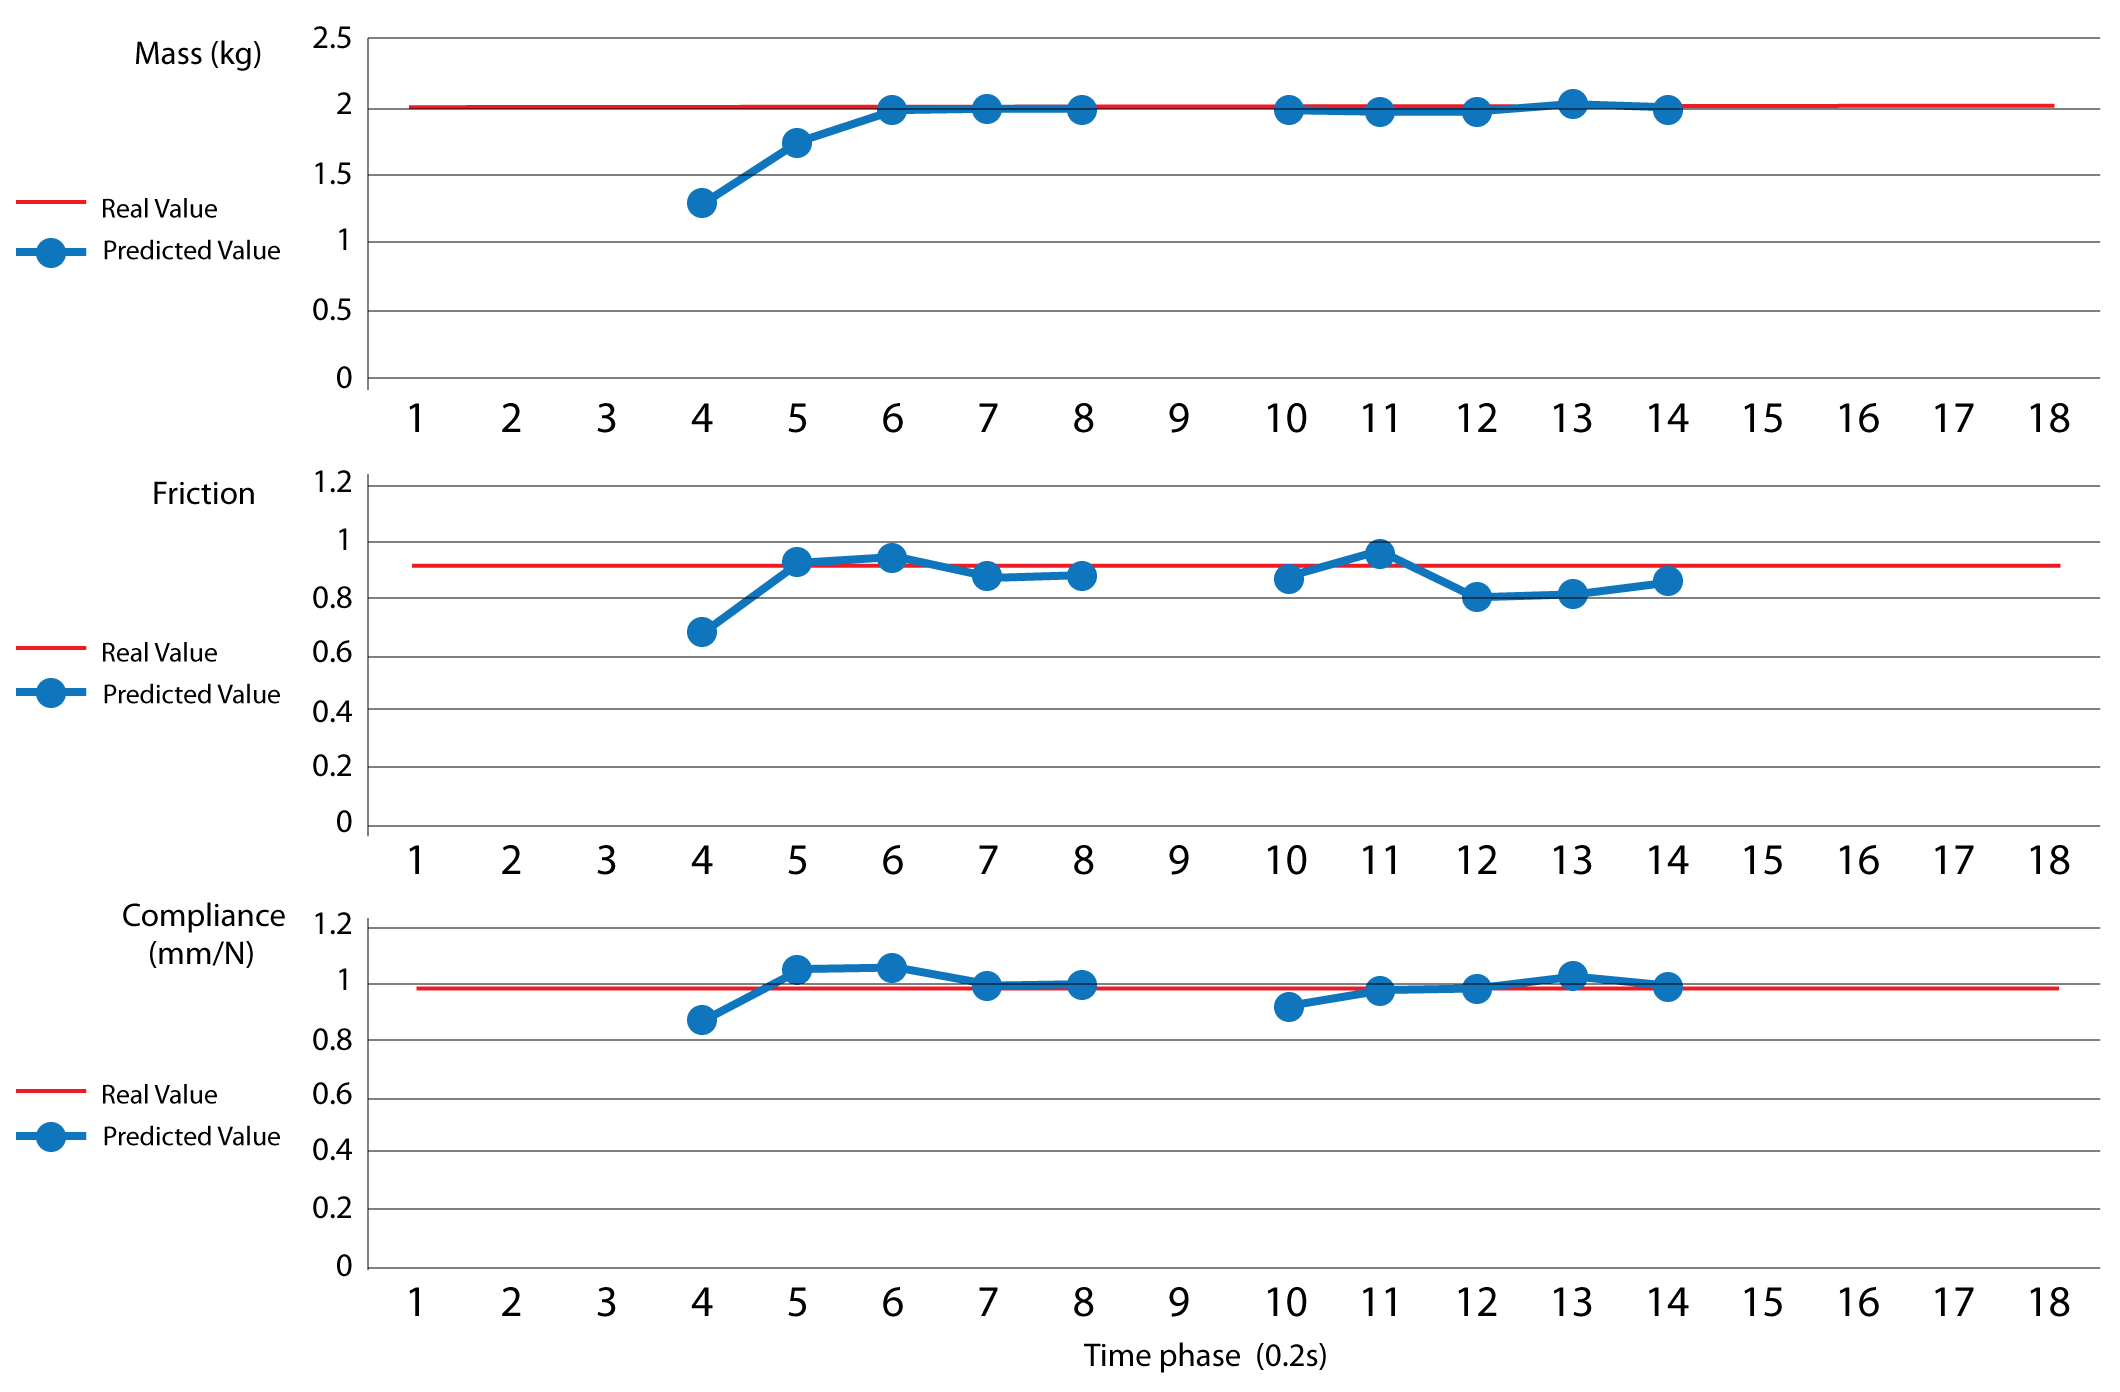
\includegraphics[width=\linewidth]{images/online_mfc_vid}
	\caption{Online estimation of mass, friction and compliance from sensory data following $\Gamma$ feature selection and PLS feature extraction. Time-phases 1 through 3, 9, and 15 through 18 are ignored since sensor readings during these time-phases do not provide any information with respect to distinguishing environment properties.}
	\label{fig:online_mfc_vid}
\end{figure}
%ENDFIGURE

\subsection{Calculating environment properties}
\label{sec:property_calc_}
In order for the robot to discover a mapping between sensor readings and environment properties, a unique numerical approximation of the underlying property must be calculated.
See Figure~\ref{fig:property_calc} for a graphical overview of how the coefficient of friction and compliance are calculated and Figure~\ref{fig:vis_properties} for a photo of each of the environmental properties.

\paragraph{Mass} 
The mass of each unit is approximated using an off-the-shelf kitchen scale.

\paragraph{Friction coefficient}
We first place the foam block atop a surface lined with the frictional material we are measuring. 
We then gradually incline the surface until the block begins to slide.
We capture the inclination at the point of sliding as $\theta$.
We finally approximate the coefficient of static friction of the frictional material to be 
$$
\mu = tan~(~\theta~), 
$$
which we also assume to be a fair approximation to the coefficient of kinetic friction.

\paragraph{Compliance}
As an estimate of the compliance of each type of foam, we set a rigid solid of known mass $m$ atop a solid block of the foam we are measuring.
The dimensions of the rigid solid and the foam solid are identical.
We then measure the compressional displacement, $d$, of the top of the foam solid using standard calipers.
Finally, we approximate the compliance of the foam to be 
$$
c = d~/~(~m~\cdot~g~),
$$ 
where $g$ is acceleration due to gravity.

\begin{figure}[]
	%\centering
    \begin{subfigure}[]{0.438\linewidth}
        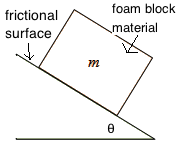
\includegraphics[width=\linewidth]{images/friction}
        \caption{Friction: ~~$\mu = tan~(~\theta~)$}
        \label{fig:friction}
    \end{subfigure}
    ~~~~
    \begin{subfigure}[]{0.490\linewidth}
        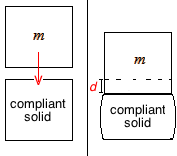
\includegraphics[width=\linewidth]{images/compliance}
        \caption{Compliance: ~~$c = d~/~(~m \cdot g~)$}
        \label{fig:compliance}
    \end{subfigure}
    \caption{Calculating numerical representations of environment properties (a) coefficient of friction, $\mu$, and (b) compliance, $c$.}
    \label{fig:property_calc}
\end{figure}

\begin{figure}[]
	%\centering
    \begin{tabular}{c}
        \begin{subfigure}[]{1\linewidth}
            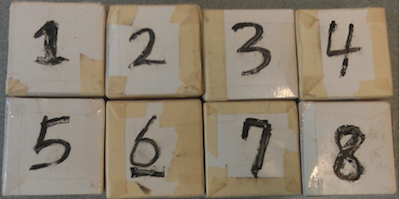
\includegraphics[width=\linewidth]{images/setup_m}
            \caption{Eight units of 0.225kg mass which are used to vary the mass of the manipulated foam block from 0.445kg to 2kg.}
        \end{subfigure} \\
        \begin{subfigure}[]{1\linewidth}
            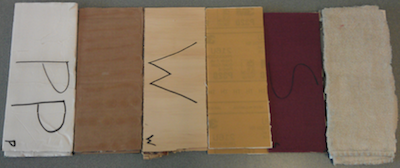
\includegraphics[width=\linewidth]{images/setup_f}
            \caption{Six surface frictions (from left to right): paper, plastic, wood, fine-sandpaper, coarse-sandpaper, cloth.}
        \end{subfigure} \\
        \begin{subfigure}[]{1\linewidth}
            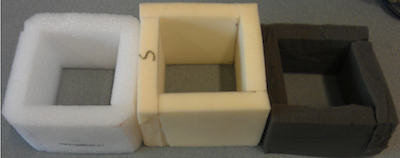
\includegraphics[width=\linewidth]{images/setup_c}
            \caption{Three levels of compliance (from left to right): ethafoam, seafoam, greyfoam.}
        \end{subfigure}
    \end{tabular}
    \caption{Environment properties used in experiments.}.
    \label{fig:vis_properties}
\end{figure}

%------------------------------------------------------------------------------------
\section{Results}
%%%%%DMT%%%%%
%%%DONE: video - label gaps in estimator output
%%%TODO: video - mark topple and slide phases on data output plots
%%%%%DMT%%%%%
In what follows below, we comment on topple-slide experiments carried out with the robot hand, as well as with the spherical probe.
We also encourage the reader to watch the supplemental video associated with this thesis.

%%%%%%%%%%%%%%%% TVR visualization

$\Gamma$ selection helps focus attention on specific sensors and motion-phases that are particularly likely to provide information useful to predicting environment properties.
Figure~\ref{fig:tvr_tables} illustrates the selected features for the topple-slide task as executed by the robot arm with either the Hand or spherical probe as end effectors (see Figure~\ref{fig:wam}).
Notice how clusters of $\mathbf{x}^*$ can be interpreted as defining important sensory events in the task sequence, which the robot should pay most attention to.
The yellow shaded region corresponds to the topple phase and the blue shaded region corresponds to the slide phase.
The motion phases where the arm is not in contact with the object are identified as being unimportant, as are the phases that mark the beginning and end of both of the topple and sliding phases.
In terms of sensors, the joint velocities, $jv_n$, are generally unimportant, with the exception of joint 6. 
Joints 2, 4, and 6 provide task-relevant information in their sensed torques and positions.
Similar results are also obtained with the full hand attached to the robot arm, in which case there are over a hundred sensors sampled across 18 time phases of the motion.
With the hand in place, the key sensors are determined as being the task wrench $\omega$, as measured by the force-torque sensor, the fingertip torques, $f$, and the fingertip tactile readings, $a$.

%FIGURE 
\begin{figure}[]
	%\centering
    \begin{center}
    \begin{tabular}{c}
        \begin{subfigure}[]{0.8\linewidth}
            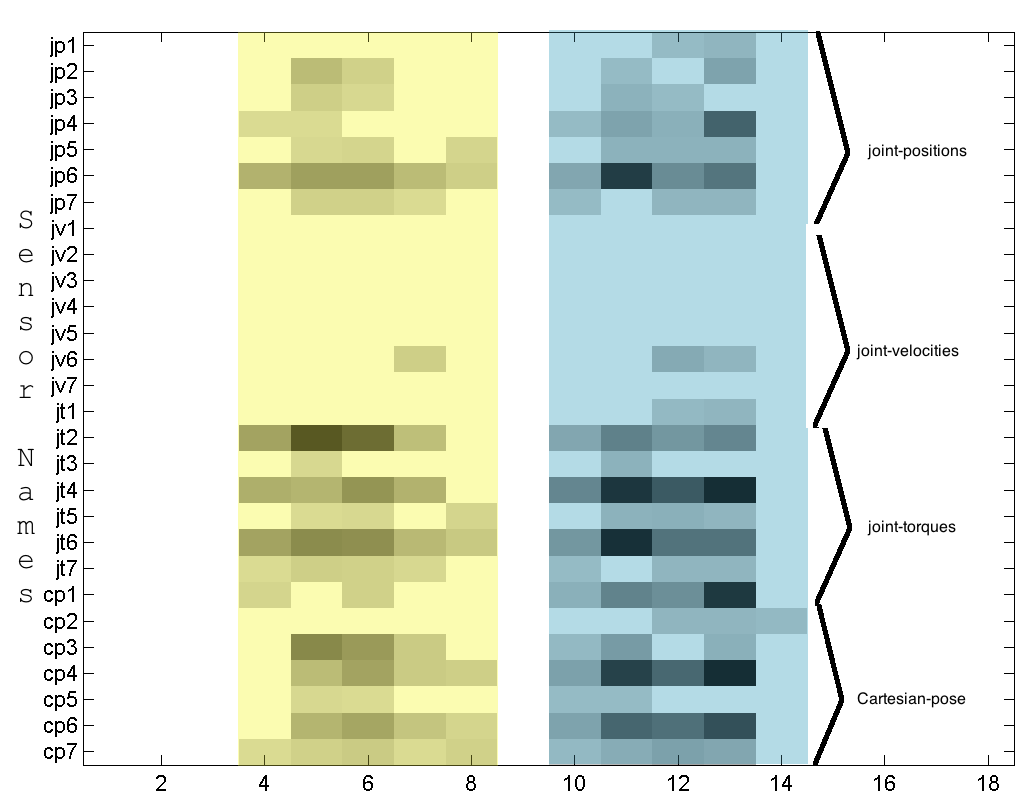
\includegraphics[width=\linewidth]{images/tvr_table_p}
            \caption{Joint-velocities are not selected due to high noise.}
            \label{fig:tvr_table_p}
        \end{subfigure}\\
        \begin{subfigure}[]{0.78\linewidth}
            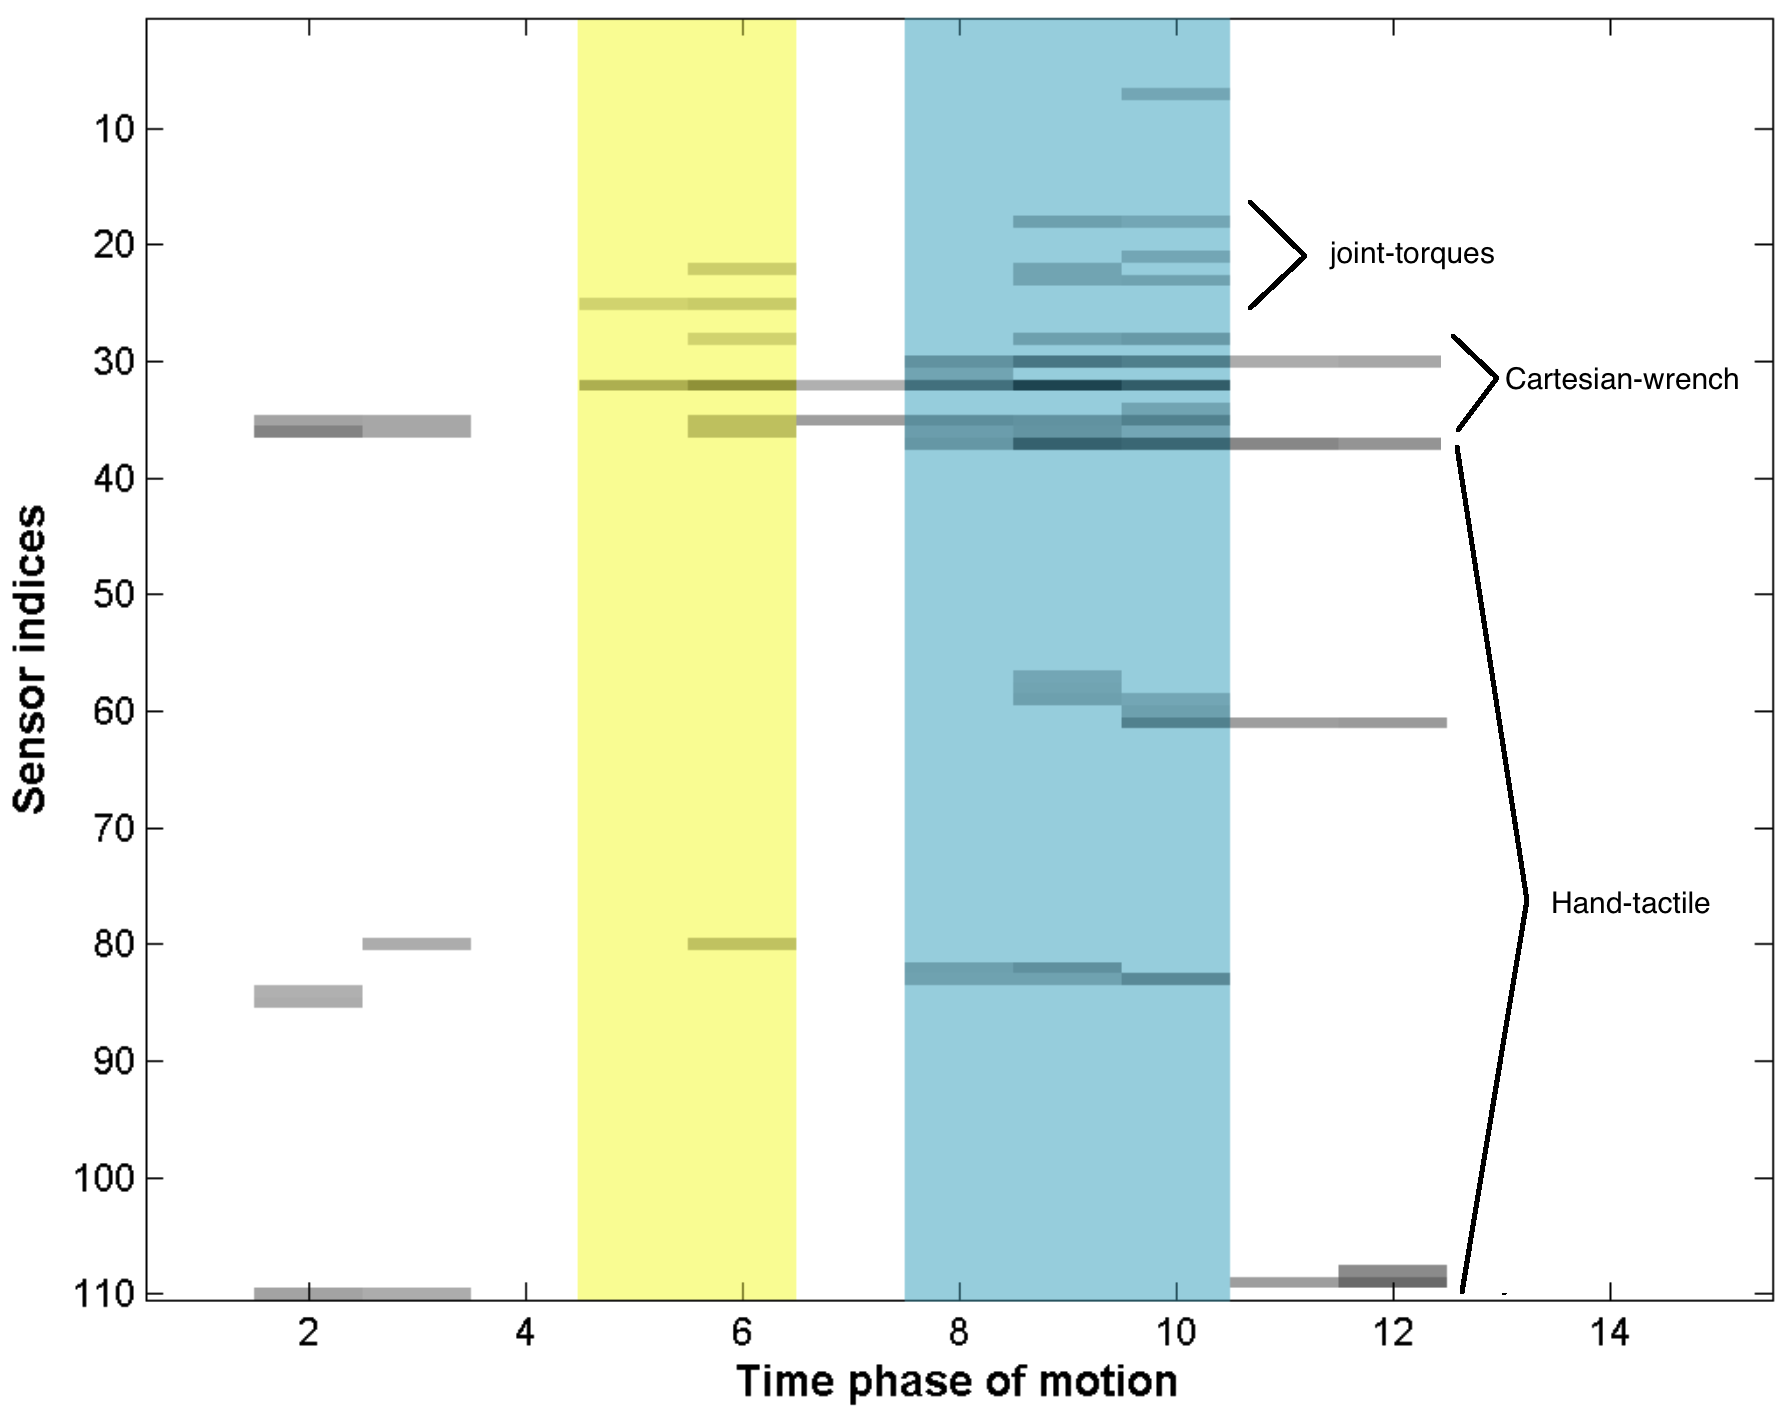
\includegraphics[width=\linewidth]{images/tvr_table_h}
            \caption{Joint-torques, Cartesian-wrench and Hand-tactile selected for providing most task-relevant information to the system.}
            \label{fig:tvr_table_h}
        \end{subfigure}
    \end{tabular}
    \end{center}
    \caption{Visualization of features selected according to the task variance ratio, $\Gamma$, of data collected using (a) robot with spherical probe and (b) robot with BarrettHand. Colour is added to signify task-phases. Gaps between task-phases signify an absence of task-relevant information within corresponding time-phases.}
    \label{fig:tvr_tables}
\end{figure}
%ENDFIGURE

\begin{figure}[]
	%\centering
    \begin{subfigure}[]{0.438\linewidth}
        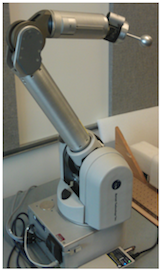
\includegraphics[width=\linewidth]{images/wam_p}
        \caption{}
    \end{subfigure}
    \begin{subfigure}[]{0.490\linewidth}
        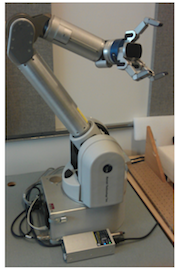
\includegraphics[width=\linewidth]{images/wam_h}
        \caption{}
    \end{subfigure}
    \caption{WAM robot with (a) spherical probe and (b) BarrettHand as end-effectors.}
    \label{fig:wam}
\end{figure}

%%%%%%%%%%%%%%%%%%
%%% DMT added: 
It may be noted that a simple contact/no-contact feature identifier might yield similar segmentations of the overall task in this case.
However, this would require an explicit model that extracts contact information from sensory inputs.
Our method identifies key points in the motion without any manually-tuned sensory features.
%%%         **Perhaps this is good material for related work section
%%%%%%%%%%%%%%%%%%

%%%DMT%%%%%%%%%%%%%
%%%TODO: compare TVR to simpler method e.g. contact no-contact thresholding
%%%DMT%%%%%%%%%%%%%
%\begin{figure}[tb]
%  \centering
%% 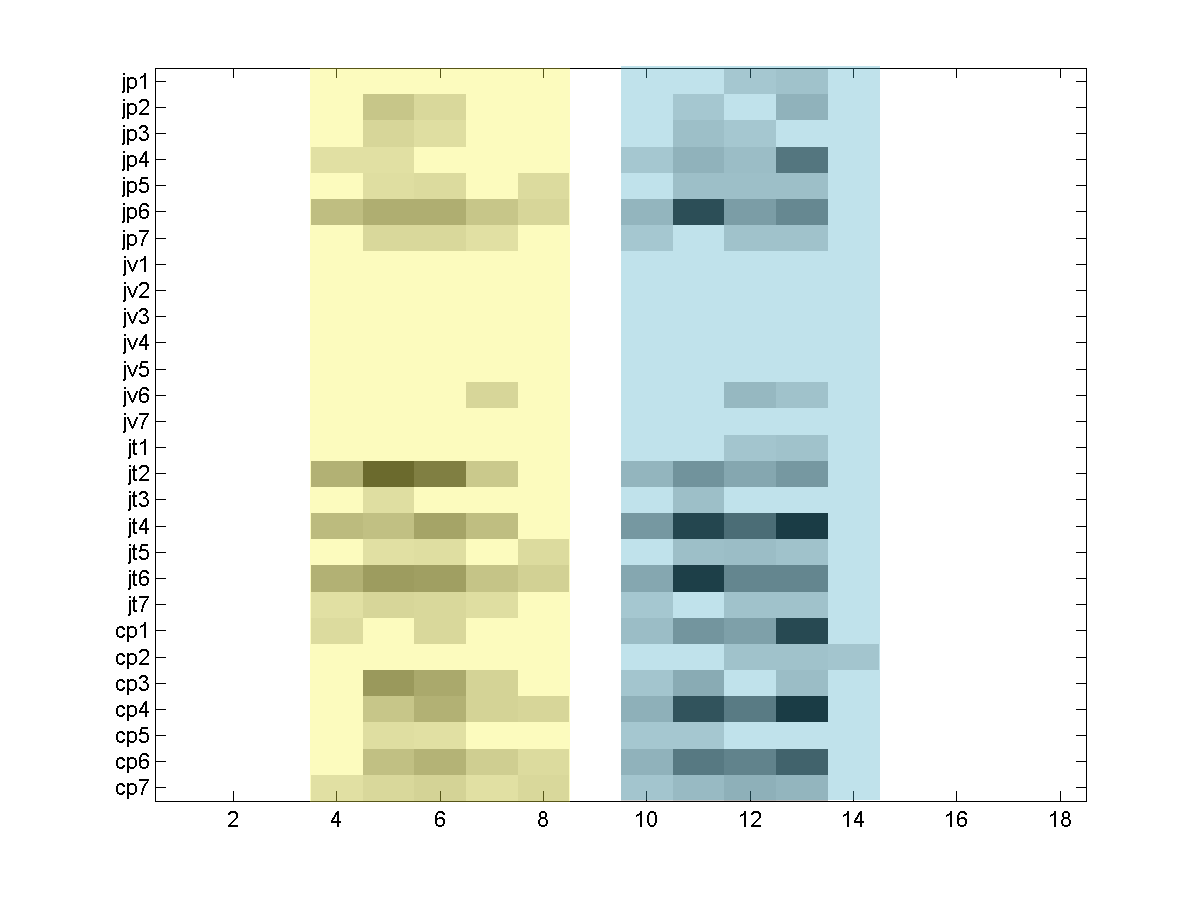
\includegraphics[width=\linewidth]{images/TVR_table}
%  \includegraphics[width=\linewidth]{images/TVR_table-probe}
%% \includegraphics[width=\linewidth]{images/TVR+photos}
%  \caption{Visualization of Task Variance Ratio ($\Gamma$) features selected for joint position (jp), velocity (jv), torque (jt), and Cartesian pose (cp) measurements. The intensity of each gray rectangular region is proportional to its $\Gamma$ value.}
%  \label{fig:TVR}
%\end{figure}


%%%%%%%%%%%%%%%%% Effect of TVR feature selection on the mass predict

%%%DMT%%%%%%%%%%%%%
%%%DONE: Error bars
%%%DONE: axis units
%%%DMT%%%%%%%%%%%%%
%\begin{figure}[tbh]
%       \centering
%%        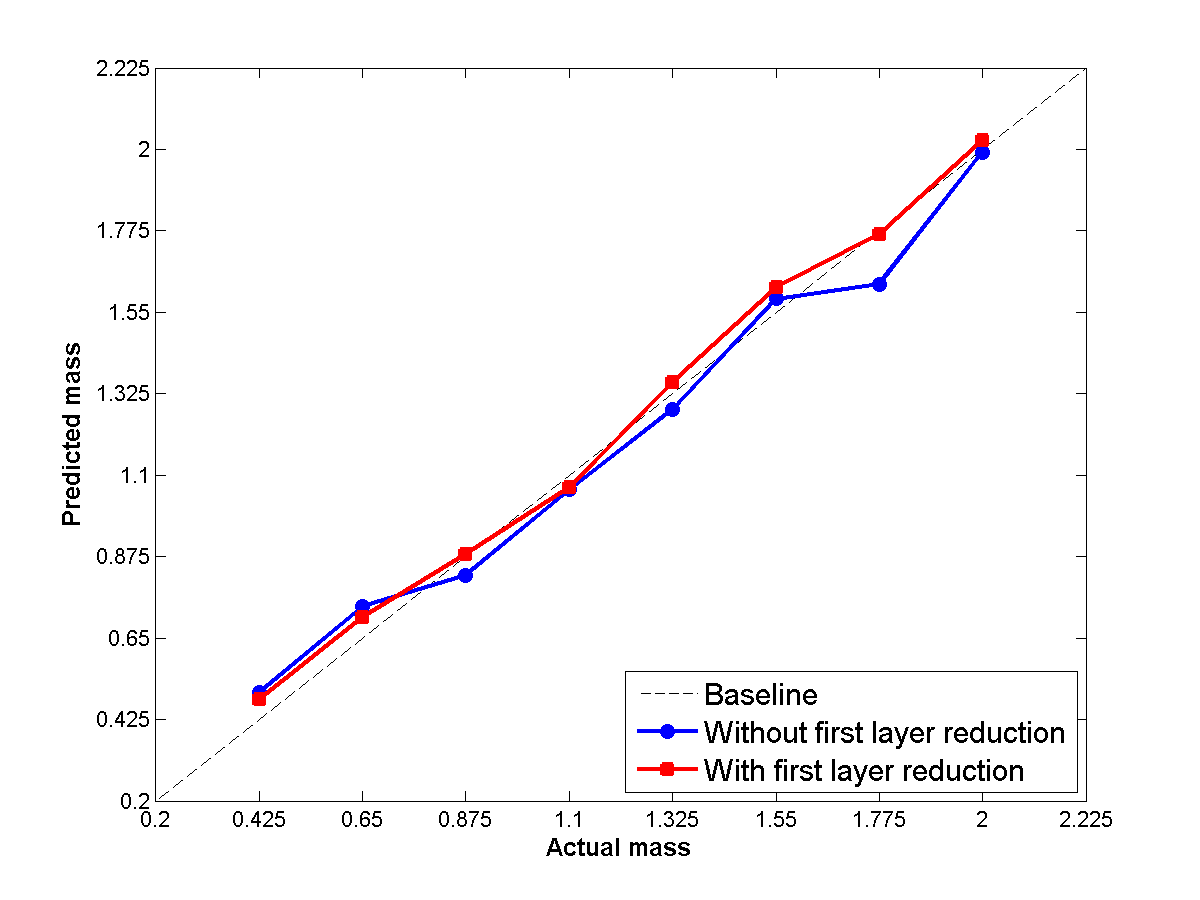
\includegraphics[width=\linewidth]{images/bomo_bomw_comp}
%       \includegraphics[width=\linewidth]{images/feature_sel_w_vs_o_bar}  %% new figure:  comparison with 10% feature selection
%       \caption{Effect of 5\% $\Gamma$ feature selection on mass predictions. Accuracy improves to within 1 measurement unit for all tests.}
%  \label{fig:TVR-perf}
%\end{figure}


To determine the impact of the $\Gamma$ feature selection, we compare mass predictions obtained using the inclusion of all features, i.e., no feature selection, and those obtained when $\Gamma$ feature selection is used to select a subset of 5\% of the the original features.
This is applied to the manipulation task as executed using the spherical probe.
In both cases, a non-reduced partial least squares model is constructed and leave-one-out-cross validation (LOOCV) test is considered for performance evaluation.
As shown in Table~\ref{tbl:TVR_perf}, the result produced using the significantly reduced subset of input features is in most tests better than that obtained when using all the features and accuracy improves to within 1 measurement unit ($\pm$ 112.5 g) for all tests.
Also, as can be seen in Table~\ref{tbl:tradeoff}, applying up to 20\% $\Gamma$ feature selection to the incoming datastreams enables real-time operation in terms of both data-transfer bandwidth and prediction runtime.
Tradeoff calculations assume 1Mbit CANBus, 16MHz dedicated processing speed and a real-time control loop frequency of 500Hz. FLOPs are calculated using standard inner-product vector multiplication complexity of $2n-1$ for each of the three property predictions.
%For experiments with the robot hand, reductions of up to 90\% using $\Gamma$-based feature selection continue to yield improvements.
%This larger reduction is possible because of the large number of tactile sensors that are available with the hand.

\begin{table}[h]
\centering
\begin{tabular}{c|c|c|}
\cline{2-3}
\multicolumn{1}{l|}{}                  & \multicolumn{2}{c|}{Prediction RMSE (g)} \\ \hline
\multicolumn{1}{|c|}{Mass (g)} & PLS + $\Gamma$    & PLS Only   \\ \hline
\multicolumn{1}{|c|}{~425}           & 2.40              & 75.7         \\
\multicolumn{1}{|c|}{~650}           & 13.9              & 86.9         \\
\multicolumn{1}{|c|}{~875}           & 1.40              & 51.1         \\
\multicolumn{1}{|c|}{1100}           & 15.8              & 40.8         \\
\multicolumn{1}{|c|}{1325}           & 7.20              & 43.1         \\
\multicolumn{1}{|c|}{1550}           & 0.20              & 37.2         \\
\multicolumn{1}{|c|}{1775}           & 9.00              & 147         \\
\multicolumn{1}{|c|}{2000}           & 11.0              & 7.20         \\ \hline
\end{tabular}
\caption{Effect of 5\% $\Gamma$ feature selection on LOOCV block mass prediction root mean squared error (RMSE). }
\label{tbl:TVR_perf}
\end{table}

%%%%%%%%%%%%%%%%%% Effect of Beta reduction on the mass predict

If desired, a fixed subset of the largest computed partial least squares coefficients can be used for the final prediction, instead of the full set, $\mathbf{\beta}$. 
In practice, a 40\% reduction in the number of coefficients yields only a minimal reduction in the quality of the prediction.

% Figure~\ref{fig:beta-perf} shows the effect of choosing increasingly small subsets of the coefficients. 
% 
% \begin{figure}[ht]
%   \centering
%   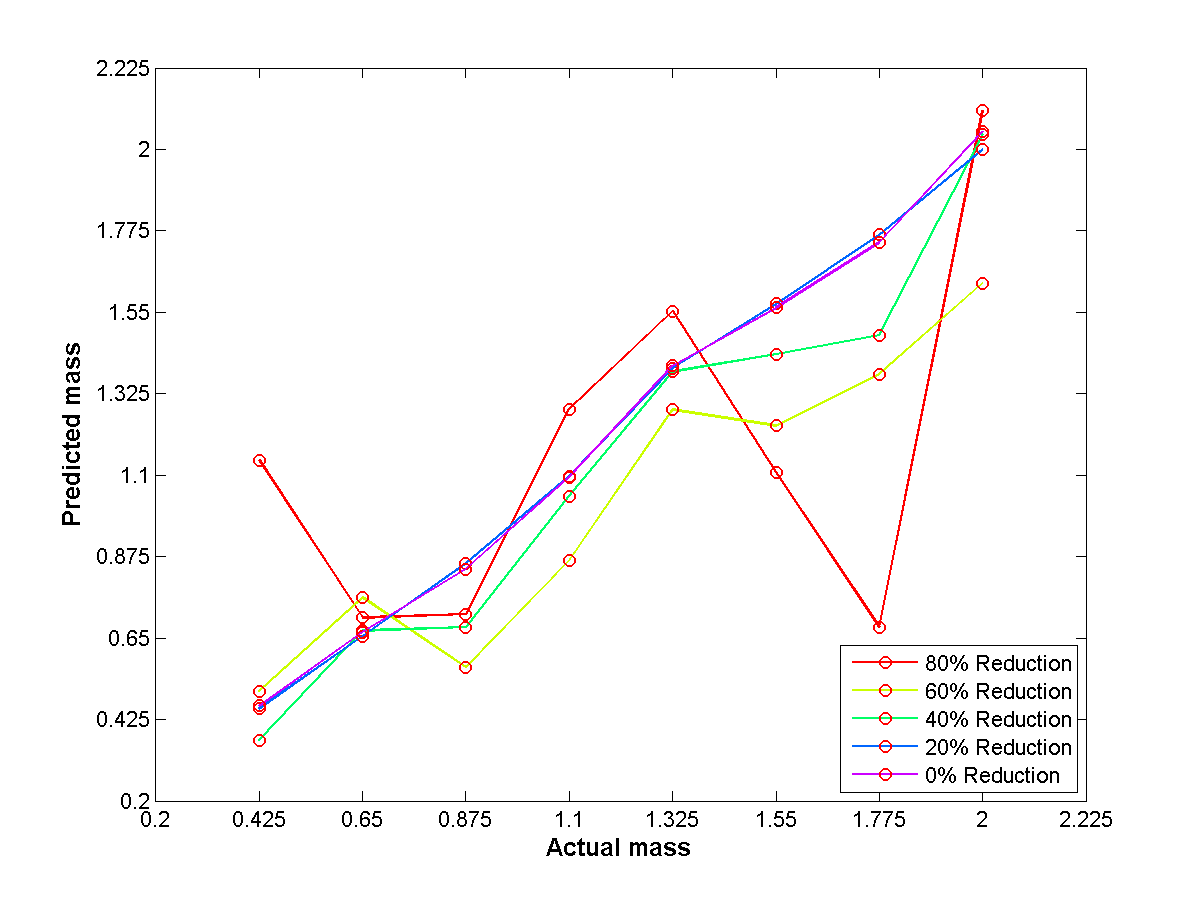
\includegraphics[width=\linewidth]{images/beta_reduc_comp}
%   \caption{Effect of partial least squares dimensionality reduction on mass prediction.}
%   \label{fig:beta-perf}
% \end{figure}

%%%%%%%%%%%%%%%%%%  Comparison to other methods

%%%DMT%%%%%%%%%%%%%
%%%DONE: Include LOOCV results in comparison (Elaborate more on generalization potential of each approach)
%%%DONE: Include mean and standard deviations for each across many runs (use dummy values for now)
%%%TODO: Replace dummy standard deviations for real ones
%%%DMT%%%%%%%%%%%%%
To validate our choice of partial least squares (PLS), we compare the results against three other methods:  principal component regression (PCR), least squares regression (LSR), and naive Bayes classification (NBC).
%In PCR, only correlations in the input space are considered when establishing a linear space for use during regression.
For LSR, we regularize the solution using ridge regression.
For NBC, a new sensory stream is treated as input to a classification problem, and the classifier is constructed using naive Bayes that assumes that all features in $\mathbf{x}$ are independent.
Using the repeated trials for the given set of environment properties, a normal distribution is constructed for each element of $\mathbf{x}$, and the likelihood of a new value of $\mathbf{x}$ belonging to the same class is simply modeled as the product of the individual element likelihoods.
The environment properties of the most likely class are then returned as the prediction.
All four methods are evaluated using LOOCV, and are applied to $\mathbf{x^*}$, i.e., after $\Gamma$ feature selection.
The results for mass prediction show that PLS yields the best predictions, with respective mean errors for PLS, PCR, and LSR and NBC of 33.3, 56.4, and 84.9, and 282.6, 
with respective standard deviations of 4.2, 8.4, 14.6 and 83.2 as measured in $grams$.

%%%%%
%%DMT removed:
%%It can be shown that PLS seeks directions of high variance \emph{and} high correlation with the response, in contrast to principal components regression, which only seeks directions of high variance.
%%%%%

%%%%%%%%%%%%%%%%%%  Online property prediction results
Figure~\ref{fig:online} illustrates online mass prediction results. The robot is able to make predictions at any key time-phase, $t^{\star}$, each characterized by a high $\Gamma$ for many sensors. This is accomplished through building multiple models, each spanning the data from the start of the motion to some $t \in t^{\star}$.
%illustrates the result for the mass predictions provided by the multiple PLS models.

These results are obtained for the case of training on data for $m = \{425, 650, 875, 1100, 1550, 1775, 2000\}$ as measured in $g$ and is then tested using sensory data obtained for $m=1335$ g.
The result shows predictions being made using increasingly fewer selected features or reduced PLS dimensions, as noted in the caption.
Also, the predictions improve as the motion progresses and more selected features are observed.  

Our framework is also robust to feature noise. To demonstrate this, we run experiments where we introduce large amounts of synthetic noise into the sensory data streams before Γ feature selection and after data whitening (see Section~\ref{sec:preprocess}). As shown in Table~\ref{tbl:add_noise}, LOOCV prediction RMSE increases smoothly as feature noise increases. Note that for even small amounts of additive noise ($\sigma^2 \approx 0.1$), PLS fails to produce meaningful results in the absence of $\Gamma$ feature selection.
%%%%%%%%DMT%%%%%%%%
%TODO: all three too similar: refocus on speedup instead of prediction performance.
%%%%%%%%DMT%%%%%%%%
%\begin{figure}[tb]
%  \centering
%  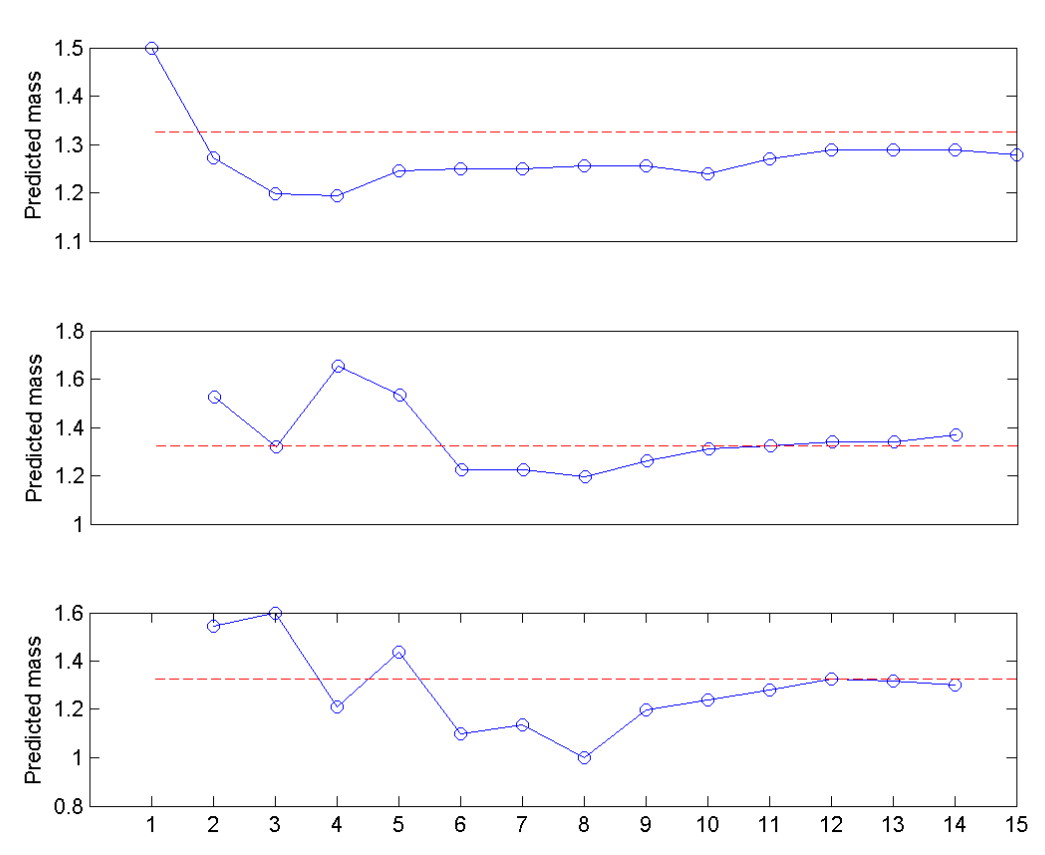
\includegraphics[width=\linewidth]{images/online_loocv_m}  %% mass predictions
%  \caption{
%    \label{fig:online}
%    Online prediction of the mass from sensory data.
%    Predictions of mass are shown at various blue points throughout the motion.
%    The dotted red horizontal line denotes the actual mass of the block.
%    The first row uses all 1650 features and no PLS reduction.
%    The second row uses a reduced set of 165 selected features without PLS reduction.
%    The third row uses 165 selected features, followed by 40\% PLS reduction.}
%\end{figure}

\begin{center}
\begin{table}[h]
\begin{tabular}{|l|l|l|l|l|l|l|}
\hline
\multicolumn{1}{|r|}{$\Gamma$ data selection:} & 5\%           & 10\%          & 20\%          & 40\%          & 70\%          & 100\%  \\ \hline
\multicolumn{1}{|r|}{\# FLOPs (approx.):}      & 32             & 65           & 131          & 263          & 461          & 659 \\ \hline
\multicolumn{1}{|r|}{Runtime (ms):}    & 0.25          & 0.5          & 1.0         & 2.1           & 3.6         & 5.1 \\ \hline
\multicolumn{1}{|r|}{Bandwidth (bit):} & 352             & 704           & 1408          & 2816          & 4928          & 7040          \\ \hline
\multicolumn{1}{|r|}{Maximum error (g):} & 69.5 & 112.7 & 96.3 & 111.4 &  107.9 & 188.3 \\ \hline
\multicolumn{1}{|r|}{\textbf{Real-time satisfied?}}        & T           & T         & T         & T/F   & F        & F        \\ \hline
\multicolumn{1}{|r|}{\textbf{Bandwidth satisfied?}}       & T           & T         & T         & F   & F        & F        \\ \hline
\multicolumn{1}{|r|}{\textbf{Accuracy satisfied?}}        & T           & T/F       & T         & T/F     & T        & F        \\ \hline
\end{tabular}
\caption{Bandwidth/runtime/accuracy tradeoff following different amounts of $\Gamma$ selection. Optimal tradeoff is achieved when between 5\% and 20\% of the data is selected using $\Gamma$.} 
\label{tbl:tradeoff}
\end{table}
\end{center}

\begin{table}[tb]
\centering
\begin{tabular}{c|c|}
\hline
\multicolumn{1}{|c|}{$\sigma^2$}   & RMSE (g)\\ \hline
\multicolumn{1}{|c|}{0.0}      & 9.4  \\
\multicolumn{1}{|c|}{0.5}      & 55.1 \\
\multicolumn{1}{|c|}{1.0}      & 160.7  \\
\multicolumn{1}{|c|}{1.5}      & 172.8  \\
\multicolumn{1}{|c|}{2.0}      & 255.5  \\ \hline
\end{tabular}
\caption{Effect of different levels of additive Gaussian noise $\mathcal{N}( 0, \sigma^2   )$ on the sensory input data for LOOCV mass prediction RMSE ($m=1335$~g). Accuracy degrades smoothly as sensor noise increases.}
\label{tbl:add_noise}
\end{table}

%---------------------------------------------------------------------------------------------------------------------
\section{Discussion}

%TODO: reorganize

Our prediction framework uses unlabeled sensory data streams, collected during a manipulation task, to make reliable real-time predictions about environment properties that cannot be visually observed, i.e., mass, friction, and compliance, given the existence of relevant training examples.
Sensors or motion phases that are observed to be noisy are readily discounted by our method.
The results show that the task variance ratio, $\Gamma$, provides a simple means for feature selection, identifying important sensors and motion-phases supporting real-time predictions, and which furthermore improves the resulting partial least squares predictions.

While predicting environment properties from labeled training data could be an obvious application of linear regression, this is in practice problematic because the training data for our scenario consists of a relatively small sample size (low hundreds) embedded in a high dimensional space: $\mathbf{x}$ can contain thousands of sensory measurements.
Furthermore, the large number of measurements required to make accurate predictions prohibits real-time operation.

Although PLS utilizes a dimension reduction technique by using a few latent factors, it cannot avoid the sample size issue since a it has been proven that a reasonable sample size relative to the number of parameters is required to estimate sample covariances consistently \cite{chun2010sparse}.
Thus, PLS works best under the conditions of large sample sizes and/or small numbers of input variables. 

When combined with $\Gamma$ feature selection, our results show PLS superior to other regression algorithms which do not leverage input and output correlations in their calculations.
Unlike PCR, PLS uses $\mathbf{y}$ (in addition to $\mathbf{x}$) to construct its principal directions.
Thus, its solution path is a nonlinear function of $\mathbf{y}$ \cite{Friedman2001}.
In addition to outperforming the other benchmark prediction methods for the task, PLS also provides a further opportunity for dimensionality reduction if desired. 

Due to the model-free nature of our approach, the prediction framework works for virtually any combination of sensor modalities, including tactile-pressure, Cartesian wrench and joint-torque, 
which enables easy experimentation to determine the optimal tradeoff between sensor usage and prediction accuracy.

One limitation of our approach is that $\Gamma$ can be misleading, such as in the case of noise-free features that also exhibit significant non-linearities with respect to the properties being predicted. 
Another drawback is that the learned predictive model remains specific to the prescribed motion used for the task and the specific kinematics and dynamics of the robot and environment it trained in.
The current remedy is to incorporate further training data from which to build the model when changes to the robot or its motion take effect.
In future work, we intend to examine how the predictive model can be transferred to new settings \cite{pan2010survey}.

Our framework can also be leveraged in multiple ways in order to detect anomalous events.
Rapid changes in the predicted environment properties, such as object compliance, is a signal of an anomaly.
Also, implicit in the computation of $\mathit{Var}^{enviro}$ is a model of what value a sensory feature should have at a given point in the motion.
This allows a motion anomaly to be signaled if a number of sensors each begin to signal anomalous values at a given point in time, or a sensor anomaly to be signaled if a single sensor begins to consistently produce anomalous readings.





%FIGURE 
%\begin{figure}[]
%	%\centering
%    \begin{center}
%	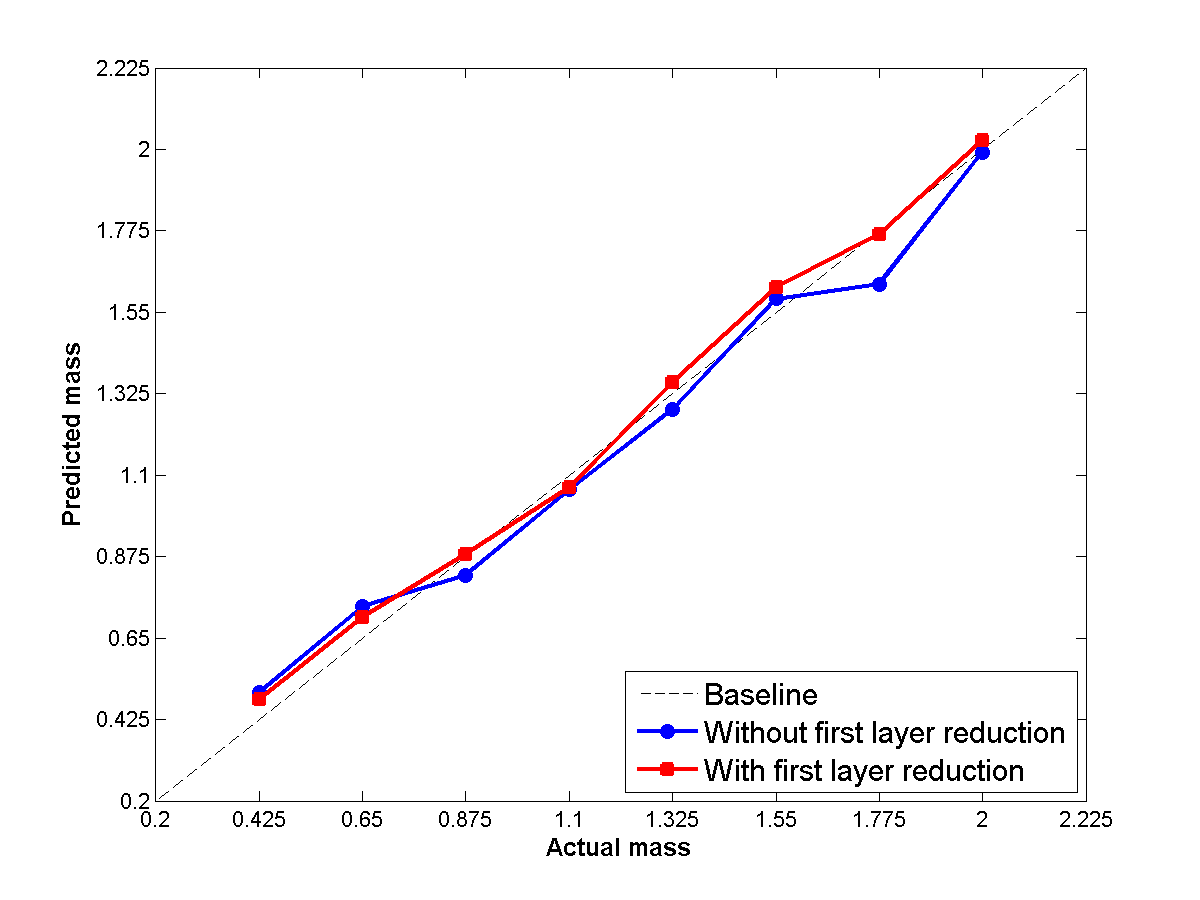
\includegraphics[width=\linewidth]{images/tvr_reduc}
%    \end{center}
%	\caption{Prediction performance of the learning system both with and without task variance ratio feature selection. Follwoing feature selection, we achieve improved performance while ignoring 75\% of the input data.}
%	\label{fig:tvr_reduc}
%\end{figure}
%%ENDFIGURE







%%%%%%%%%%%%%%%%%%%%%%%%%%%

\chapter{Conclusions and Future Work}
\label{chap6}
%\section{Future Directions}

In the thesis, I present the challenge of predicting properties of real-world environments using high-dimensional haptic sensory data from the perspectives of both biological and robotic systems.

\section{Summary}

I begin in Chapter~\ref{chap2} by presenting insights into the problem from the established robotics, neuroscience and physiology literature. 
Next, I define the prediction problem more formally in Chapter~\ref{chap3}.
In Chapter~\ref{chap4} I provide an overview on the software framework used to control the physical WAM/Hand system and collect data in support of experiments.
I then introduce a model-free approach to the prediction of example environment properties -- namely object mass, friction, and compliance -- during the course of a non- prehensile topple-slide manipulation task in Chapter~\ref{chap5}.

Given appropriate data from example manipulations with known environment properties, the method  presented in the thesis extracts information from unlabeled sensory data collected over the course of a new manipulation. 
I demonstrate that our novel metric, known as the Task Variance Ratio (TVR), identifies important features, sensors and motion-phases. 
Using the TVR metric combined with the PLS regression method, we obtain accurate predictions in real-time using only 3\% of the sensory input data from the robot. 

\section{Limitations and Future Directions}
% limitations and future work: prescribed motion, fixed timing, kinematic and dynamic generalization

One significant limitation of the predictive framework is the need for a prescribed motion that can already succeed at the task despite variations in the environment properties that I seek to predict.
%A related issue is the need for the motion to run in open-loop and is not sensitive to any kind of obstruction, as may be encountered in dynamic environments.

An important direction for future work will be to investigate the tight integration of prediction and adaptation into the framework.  
With knowledge (learned or provided) of how to adapt the topple-slide task for heavier or more compliant blocks, this could readily be used to enlarge the range of variations that can be coped with. 

\subsection*{Surprise-and-adapt}
I have devised a preliminary model-based motion adaptation approach to succeed in environments where the prescribed motion fails.
Under the assumption that the robot has access to tactile pressure and/or fingertip torque sensors, I modify the orientation of the robot's wrist about the axis parallel to the manipulated block, so that the pressure readings at the fingertips track an appropriate profile provided by an expert.

To deal with sensor noise, I consider a history of sensor readings of size $K_r$.
If sensor readings fall below a threshold for at least $K_r$ timesteps, the orientation of the wrist increases -- thus applying more pressure to the block.
Similarly, if sensors consistently read above a threshold, the orientation of the wrist decreases -- releasing pressure.
See Program~\ref{pgm:saa} for a pseudocode of this operation.

This scheme is successful for the topple-slide task when particularly small perturbations in the environment are experienced, such as a relatively small (within two units) change in object mass, but fails with large perturbations.%, such as if the block is removed completely from the workspace.

An interesting future direction is to devise a model-free approach in which the robot discovers for itself that a lack of pressure at its fingertips means that its wrist orientation should increase (in addition to other relevant mappings between sensor readings and adaptive motions).
This knowledge would have to come from the data and would most likely require additional sensors and/or some form of supervision, e.g. from a human or a camera.

\begin{Program}[width=0.5\linewidth]
\center
\begin{verbatim}
void operate()  //repeat at 500Hz
{   //Consider a history of thresholded differences.
    if ( sensor_value - expected_value > threshold_p )
        history.append_front ( 1 )
    else if ( sensor_value - expected_value < threshold_n )
        history.append_front ( -1 )
    else
        history.append_front ( 0 )
    //'Surprise' iff at least K contiguous unexpected readings.
    if ( sum ( history [ 0 : K ] ) == K )   //too much pressure
        decrease_wrist_angle()
    if ( sum ( history [ 0 : K ] ) == -K )  //too little pressure
        increase_wrist_angle()
}
\end{verbatim}
%signal ( ADAPT )    // adapts to new environment
%if ( surprise_and_adapt )       // OR 
%if ( surprise_and_stop )
%    signal ( STOP )     // robot stops operation
  \caption{Realtime \emph{operate} method pseudocode for the surprise-and-adapt realtime system module. See Section~\ref{sec:realtime_eg} for general details on Libbarrett realtime systems development.}
  \label{pgm:saa}
\end{Program}


\subsection*{Time-synchronized motions}

A related limitation is that our current sensory features are all time-indexed, i.e., there is an assumption that the current phase of the motion is tightly coupled to the current time.  In future work, I would like to couple the phase estimate more tightly to the actual motion via available sensory observations.

\subsection*{Task-parameter generalization}

A last key limitation is that because of the model-free nature of the current approach, the prediction procedures do not generalize well to changes in the task kinematics or dynamics. 
I aim to develop parameterized versions of the predictive model in order to allow for such generalization.

\subsection*{Leveraging physics-based simulation}

I am are also interested in exploring how simulations with only qualitative accuracy might be used to identify suitable sensors and motion phases in advance. This could be used to inform the types of sensors and their placement, as well as provide insight with respect to relevant time-steps at which to record data.  Initial results in this direction are promising and thus point to a new use for simulations that are not necessarily tightly calibrated to the true kinematics and dynamics of the plant.

%%%%%%%%%%%%%%%%%%%%%%%%%%%

%\input{report}

\bibliographystyle{plain}
\bibliography{allbibs}

\appendix
\input{software}
%\chapter{Hardware Overview}

%\section{Theory of Operation} 

%We begin this section with an overview of the equipment (i.e. the WAM and BarrettHand) followed by a brief look at how this equipment is monitored and controlled throughout the experiments.

\section{Whole Arm Manipulator (WAM)} 

The WAM is a 7 degree-of-freedom (DOF) robotic arm and wrist system from Barrett.
There are three input types when controlling the WAM: (1) joint position, (2) joint torque, and (3) Cartesian position.
All inputs are automatically translated into joint torques and fed to puck motors in the arm [40].
The simplest control input is Cartesian (X, Y, Z) however it does not guarantee exact positioning within the robot’s Cartesian workspace (approximated as a 2-meter diameter sphere), nor does this control scheme support any kind of collision avoidance.
In contrast, joint-space input offers complete and accurate control over all DOFs of the arm.

The WAM is PID-controlled in realtime mode whereas all other function is non-realtime.
This poses some restrictions on controller execution.
For example, output to the console during realtime operation is forbidden and forces the control program to halt.
The WAM comes with built-in gravity compensation mode, which, when active, adds a high level of compliance to the arm.

See Figure 3.2 for the WAM’s joint angle and velocity/acceleration limits and Figure 3.3 for further specifications.

\section{Force/Torque Sensor} 

The Barrett 6-Axis Force/Torque Sensor expands the force sensing capability of the WAM and BarrettHand systems.
The Force/Torque sensor processes signals from all the strain gages and outputs three forces and three torques within the Cartesian workspace of the WAM.
Full specifications are presented in Figure 3.5.

\section{BarrettHand} 

The BarrettHand is a 4 DOF, under-actuated, threefingered robotic hand from Barrett.
The DOFs are the joint positions at the base of each finger, and the spread of the first and second fingers around the circumference of the wrist.
See Figure 3.7 for details. 
The hand’s underactuation is possible via the TorqueSwitch technology, which is presented in Figure 3.6.
The hand is controlled in four fashions: (1) joint-torques; (2) joint-velocitie; (3)
joint-positions; and (4) high-level commands.
Jointposition commands are executed with a trapezoidal motion profile meaning that accelerations change instantaneously at the point the command is given.
High-level commands include commanding any or all fingers to open or close.
As with the WAM, all commands are eventually translated to joint-torques by the associated puck motors in the hand [41].
Apart from standard joint-encoders, the BarrettHand has optional sensors, which include tactile and strain-gage sensors.

\subsection{Tactile Sensors} 

Tactile sensors onboard the BarrettHand localize pressure across the palm and fingers.
They are arranged as four sets of cell arrays; one set within the distal segment of each finger as well as one set in the palm.
There are 96 cells in total (24 in each set).
See Figure 3.11 for full tactile sensor specifications.

\subsection{Strain-gage Sensors} 

Strain in the hand is measured as torques experienced about the distal joints of each of the hand’s fingers over a range of +/- 1 N-m.
Strain-gages measure the differential tension in the tendon-like structure running through each finger to the second joint.See Figure 3.8 for a schematic drawing of the joint-torque sensor system of the hand.


\backmatter

%% Indices come here if you have them.

\end{document}
\endinput
